%%%%%%%% 1. DOCUMENTCLASS %%%%%%%%
% Choose the language of your thesis passing 'french' or 'english' as
% \documentclass option.
% Note1: The 'page de garde' will always be written in French.
% Note2: You will have an error if you change the language of the document and
%        compile it without cleaning the auxiliary files. Compiling it again
%        should solve the problem.
\documentclass[english,a4paper,11pt,twoside]{StyleThese}


%%%%%%%% 2. PACKAGES AND BASIC INFO %%%%%%%%
\usepackage[T1]{fontenc}
\usepackage[utf8]{inputenc}
\usepackage{datetime} % For month display
\usepackage{lmodern} % Font Latin Modern Roman
\usepackage{tabularx} % Table
\usepackage{multirow} % Table multirow

\iftoggle{ThesisInEnglish}{%
  \usepackage[english]{babel}
}{ %
  \usepackage[english,main=french]{babel}
}

\usepackage{hhline}
\usepackage[left=1.5in,right=1.3in,top=1.1in,bottom=1.1in,includefoot,includehead,headheight=13.6pt]{geometry}
\renewcommand{\baselinestretch}{1.05}

% Math
\usepackage{amsmath,amssymb}

%%%%%%%% Table of contents %%%%%%%%
\setcounter{secnumdepth}{3}
\setcounter{tocdepth}{2}

% Table of contents for each chapter
\usepackage[nottoc, notlof, notlot]{tocbibind}
\usepackage{minitoc}
\setcounter{minitocdepth}{2}
\mtcindent=15pt

% Use \minitoc where to put a table of contents
\let\minitocORIG\minitoc
\renewcommand{\minitoc}{\minitocORIG \vspace{1.5em}}

% Glossary / list of abbreviations
\usepackage[intoc]{nomencl}
\iftoggle{ThesisInEnglish}{%
  \renewcommand{\nomname}{Glossary}
}{ %
  \renewcommand{\nomname}{Liste des abréviations}
}
\makenomenclature

% \usepackage[acronym]{glossaries}
% \makeglossaries


%%%%%%%% Image %%%%%%%%
\usepackage{ifpdf}

\ifpdf
  \usepackage[pdftex]{graphicx}
  \DeclareGraphicsExtensions{.jpg}
  \usepackage[pagebackref,hyperindex=true]{hyperref}
  \usepackage{tikz}
  \usetikzlibrary{arrows,shapes,calc}
\else
  \usepackage{graphicx}
  \DeclareGraphicsExtensions{.ps,.eps}
  \usepackage[dvipdfm,pagebackref,hyperindex=true]{hyperref}
\fi

\usepackage{rotating} % Sideways of figures & tables
\usepackage{tablefootnote}


%%%%%%%% PDF %%%%%%%%
% Links in pdf
\usepackage{color}
\definecolor{linkcol}{rgb}{0,0,0.4}
\definecolor{citecol}{rgb}{0.5,0,0}
\definecolor{linkcol}{rgb}{0,0,0}
\definecolor{citecol}{rgb}{0,0,0}
% Change this to change the informations included in the pdf file

% Basic pdf setup
\hypersetup
{
  bookmarksopen=true,
  %pdftoolbar=false, %barre d'outils non visible
  pdfmenubar=true, %barre de menu visible
  pdfhighlight=/O, %effet d'un clic sur un lien hypertexte
  colorlinks=true, %couleurs sur les liens hypertextes
  pdfpagemode=UseNone, %aucun mode de page
  pdfpagelayout=SinglePage, %ouverture en simple page
  pdffitwindow=true, %pages ouvertes entierement dans toute la fenetre
  linkcolor=linkcol, %couleur des liens hypertextes internes
  citecolor=citecol, %couleur des liens pour les citations
  urlcolor=linkcol %couleur des liens pour les url
}


%%%%%%%% Backref in biblio %%%%%%%%
%% Nicer backref links
\iftoggle{ThesisInEnglish}{%
  \renewcommand*{\backref}[1]{}
  \renewcommand*{\backrefalt}[4]{%
  \ifcase #1 %
  (Not cited.)%
  \or
  (Cited in page~#2.)%
  \else
  (Cited in pages~#2.)%
  \fi}
  \renewcommand*{\backrefsep}{, }
  \renewcommand*{\backreftwosep}{ and~}
  \renewcommand*{\backreflastsep}{ and~}
}{%
  \renewcommand*{\backref}[1]{}
  \renewcommand*{\backrefalt}[4]{%
  \ifcase #1 %
  (Non cité.)%
  \or
  (Cité en page~#2.)%
  \else
  (Cité en pages~#2.)%
  \fi}
  \renewcommand*{\backrefsep}{, }
  \renewcommand*{\backreftwosep}{ et~}
  \renewcommand*{\backreflastsep}{ et~}
}

\usepackage{xurl} % allow break url

%%%%%%%% Fancy Header %%%%%%%%
% Fancy Header Style Options
\usepackage{fancyhdr}                   % Fancy Header and Footer
\pagestyle{fancy}                       % Sets fancy header and footer
\fancyfoot{}                            % Delete current footer settings

\fancyhead[LE,RO]{\bfseries\thepage}    % Page number (boldface) in left on even
                                        % pages and right on odd pages
\fancyhead[RE]{\bfseries\nouppercase{\leftmark}}      % Chapter in the right on even pages
\fancyhead[LO]{\bfseries\nouppercase{\rightmark}}     % Section in the left on odd pages

\let\headruleORIG\headrule
\renewcommand{\headrule}{\color{black} \headruleORIG}
\renewcommand{\headrulewidth}{1.0pt}
\usepackage{colortbl}
\arrayrulecolor{black}

\fancypagestyle{plain}{
  \fancyhead{}
  \fancyfoot{}
  \renewcommand{\headrulewidth}{0pt}
}


%%%%%%%% Clear Header %%%%%%%%
% Clear Header Style on the Last Empty Odd pages
\makeatletter
\def\cleardoublepage{\clearpage\if@twoside \ifodd\c@page\else%
  \hbox{}%
  \thispagestyle{empty}%              % Empty header styles
  \newpage%
  \if@twocolumn\hbox{}\newpage\fi\fi\fi}
\makeatother


%%%%%%%% Center Page %%%%%%%%
% centered page environment (for abstract)
\newenvironment{vcenterpage}
{\newpage\vspace*{\fill}\thispagestyle{empty}\renewcommand{\headrulewidth}{0pt}}
{\vspace*{\fill}}


%%%%%%%% End Common Format %%%%%%%%


% Loading the tlsflyleaf.sty package require some option to define the
% establishment name, the doctoral school and the PhD speciality.
% In that aim you have 2 key-value option:
%   - Ets=<value> : define the establishment name
%   - ED=<value>  : define the doctoral school and speciality
%   - ED2=<value> : define the second speciality ("double mention"). OPTIONAL.
% The full list of accepted values for each option could be find either
% in the documentation or in tlsflyleaf.sty file.
%\usepackage[ED=MITT-STICRT, Ets=INSA]{tlsflyleaf}
%\usepackage[ED=SDU2E-Ast, ED2=SDU2E-Eco, Ets=UT3]{tlsflyleaf}
\usepackage[ED=EDSYS-A, Ets=ENAC]{tlsflyleaf}

% Setup basic string
\title{Titre de la th\`ese}
\author{Florian SANSOU}
\defencedate{jj/mm/aaaa}
\lab{Ecole Nationale d’Aviation Civile}
%\cotutelle{}

% Setup custom pdf info
\makeatletter
\hypersetup {
  pdftitle={\@title},
  pdfauthor={\@author},
  pdfsubject={Thesis subject},
  pdfkeywords={key, words},
}
\makeatother

% Setup people like your boss, the jury team and the referees
% - First you need to define how number they will be in each category
%   It is done with the commands \nboss{n}, \nreferee{n} and \njudge{n}.
%   You can define more people in each category than the number given
%   but only the first "\npeople" will be print.
% - Then use the command \makesomeone{<category>}{<number>}{<name>}{<status>}{<other>}
%   where:
%     <category> should be select in ['boss', 'referee', 'judge']
%     <number>   is the rank for printing the person.
%                Only number <= "\npeople" will be printed
%     <name>     First name and las name of the people
%     <status>   Is (s)he a "charg\'e de recher" ou un "professeur d'universit\'e"...
%     <other>    What ever string you want to add (laboratory, jury member place...).
%% Boss
\nboss{2}
\makesomeone{boss}{2}{Second DIRECTEUR}{}{}  % Sera affiche en second
\makesomeone{boss}{1}{Premier DIRECTEUR}{}{} % Sera afiche en premier
%% Referee
\nreferee{2}
\makesomeone{referee}{1}{Premier RAPPORTEUR}{}{}
\makesomeone{referee}{2}{Second RAPPORTEUR}{}{}
%% Judges
\njudge{5}
\makesomeone{judge}{1}{Premier MEMBRE}{Professeur des universit\'es}{Pr\'esident du jury}
\makesomeone{judge}{2}{Second MEMBRE}{Ing\'enieur de recherche}{Rapporteur}
\makesomeone{judge}{3}{Troisi\`eme MEMBRE}{Charg\'e de recherche}{Examinateur}
\makesomeone{judge}{4}{Quatri\`eme MEMBRE}{Ma\^itre de conf\'erences}{Co-directeur de th\`ese}
\makesomeone{judge}{5}{Ciqui\`eme MEMBRE}{Directeur de recherche}{Directeur de th\`ese}

% Other package here
% ...

\sloppy
\begin{document}

%%%%%%%% 3. COVER PAGE %%%%%%%%

\makeatletter
\pdfbookmark{\@title}{title}
\makeatother

\makeflyleaf
% 
\includepdf[pages=-]{chapters/couverture_these.pdf} % if you want to use generated pdf cover (e.g. ADUM), use this instead of \makeflyleaf. You'll also need \usepackage{pdfpages}
\cleardoublepage
\dominitoc


%%%%%%%% 4. ACKNOWLEDGMENTS AND TABLES OF CONTENT %%%%%%%%
\pagenumbering{roman}
% Here you can see an example of how to create text conditioned by the language
% variable. The \iftoggle command:
%
%   \iftoggle{ThesisInEnglish}{%
%   <your-text-in-english>
%   }{%
%   <your-text-in-french>
%   }
%
% will compile only one of the two blocks, depending on the variable you set at
% the beginning of this document. Language selection is managed this way in the
% formatAndDefs.tex file. You too can create sections of your thesis that is
% language dependend this way, although you probably won't need it. Another use
% of \iftoggle can be found at the end of this file.
\iftoggle{ThesisInEnglish}{%
\section*{Acknowledgments}
}{%
\section*{Remerciements}
}

\todo{Remerciement}
Un tel travail aurait été impossible à réalisé sans la gentillesse d'autres personnes. Mes remerciements vont d'abord à Paolo ROBUFFO GIORDANO et Pascal MORIN, qui ont accepté de relire cette thèse et d'en être rapporteur. La version définitive de ce mémoire a bénéficié de leur lecture très attentive et de leurs remarques précieuses. Je tiens à remercier Sophie TARBOURIECH d’avoir accepté d’être présidente du jury. Je remercie également Philippe CHEVREL d’avoir accepté d’assister à la présentation de ce travail et de s’être déplacé depuis Nantes.

Je voudrais remercier tout particulièrement Luca ZACCARIAN

\cleardoublepage
\pdfbookmark{\contentsname}{toc}
\tableofcontents

\renewcommand{\listfigurename}{Liste des figures}
\listoffigures
\addcontentsline{toc}{chapter}{\listfigurename}
\mtcaddchapter

\listoftables
\addcontentsline{toc}{chapter}{\listtablename}
\mtcaddchapter

\printnomenclature
% Use \mtcfixnomenclature below if you have a glossary (added with
% \printnomenclature above) and you're see a shift in the mini-table of
% contents at the begining of each chapter (example: no mini-toc in chapter 1;
% mini-toc of chapter 1 appearing in chapter 2; and so on).
%
% You should not use \mtcfixnomenclature if you have no glossary (that means,
% if you don't use \printnomenclature or if your glossary is empty).
\mtcfixnomenclature


%%%%%%%% 5. MAIN CONTENT %%%%%%%%
\mainmatter

\chapter*{Introduction}
\addstarredchapter{Introduction} %Sinon cela n'apparait pas dans la table des matières
\markboth{Introduction}{Introduction} % headers


\section*{Contexte}
Ces dernières années, le domaine des drones s'est considérablement développé. En effet, de nombreux progrès ont été réalisés dans la conduite de vols autonomes, lesquels permettent de réaliser de nombreuses tâches longues, répétitives ou dangereuses, de manière plus sûre que des avions ou des systèmes télépilotés. Les drones ont fait leurs preuves dans de nombreuses applications civiles, alors qu'ils étaient auparavant conçus à des fins de surveillance et de destruction dans le secteur militaire. Tout leur intérêt réside dans leur capacité à se maintenir stabilisé sans intervention humaine. Ainsi, les opérateurs peuvent se concentrer sur la mission, sans devoir consacrer une grande attention au pilotage du drone. 

La possibilité d'utiliser des systèmes de vols autonomes dans le secteur civil a été rendue possible par l'accessibilité croissante, proposée par l'industrie, de solutions à faible coût pour les applications d'imagerie aérienne. Ainsi, ce sont dans des domaines aussi variés que l'agriculture de précision,  l'inspection des infrastructures civiles ou encore les opérations de sécurité que les drones autonomes sont aujourd'hui mobilisés, devenant alors un riche sujet de recherche.

La miniaturisation des équipements électroniques et mécaniques est à l'origine de l'essor d'une classe de drones de plus en plus petits. Souvent qualifiés de \textit{Micro Air Vehicle} (MAV) ou de \textit{Unmanned Aerial Vehicle} (UAV), leur petite taille leur permet d'intervenir dans des espaces confinés ou contraints. Ils n'ont, cependant, qu'une charge utile restreinte, souvent limitée à l'emport d'une caméra ou d'un colis de faible masse. Leur faible autonomie restreignant leur usage, la recherche s'est alors concentrée sur une solution permettant d'optimiser leur utilisation. En cela, les drones à décollage et atterrissage verticaux (\textit{Vertical take-off and landing}; VTOL) répondent aux exigences.
\nomenclature[]{\(VTOL\)}{Drones à décollage et atterrissage verticaux (\textit{Vertical Take-Off and landing})}
\nomenclature[]{\(MAV\)}{Micro drone (\textit{Micro Air Vehicle})}
\nomenclature[]{\(UAV\)}{Drone autonomes (\textit{Unmanned Aerial Vehicle})}

Dans l'ensemble des VTOL, plusieurs architectures existent et seront détaillées dans la section \ref{sec:archConvertible}. Toutefois, nos travaux se sont concentrés sur les classes des \textit{tailsitters} et des \textit{freewings}.

\subsection*{Phases d'un vol}
De nombreux travaux ont été menés sur les \textit{tailsitters}, avec l'objectif de couvrir l'intégralité du domaine de vol. Ce dernier est constitué des phases de vol suivantes :
\begin{enumerate}
    \item Décollage vertical
    \item Transition entre le vol stationnaire et le vol d'avancement
    \item Vol d'avancement
    \item Transition entre le vol d'avancement et le vol stationnaire
    \item Atterrissage vertical
\end{enumerate}


Bien que l'on puisse observer une symétrie entre la phase \raisebox{.5pt}{\textcircled{\raisebox{-.9pt} {1}}} et \raisebox{.5pt}{\textcircled{\raisebox{-.9pt} {5}}}, qui correspondent au décollage et à l'atterrissage vertical, une différence fondamentale est notable. Lors du décollage, la vitesse du drone engendrera un flux d'air sur l'aile, orienté dans le même sens que le flux d'air généré par les hélices. Cependant, lors de l'atterrissage, le flux d'air va se trouver inversé, le drone devant descendre, ce qui engendrera une vitesse opposée à la direction du flux d'air des hélices. Cette inversion génère une instabilité qui doit être compensée par le contrôleur.

Le vecteur $\overrightarrow{W}$ représente la perturbation de vent qui peut affecter le vol sur l'intégralité des cinq phases de vol. Toutefois, on observe que dans les phases de décollage \raisebox{.5pt}{\textcircled{\raisebox{-.9pt} {1}}}, de transition \raisebox{.5pt}{\textcircled{\raisebox{-.9pt} {2}}} et \raisebox{.5pt}{\textcircled{\raisebox{-.9pt} {4}}} et d'atterrissage \raisebox{.5pt}{\textcircled{\raisebox{-.9pt} {5}}}, le drone offre une grande surface verticale sujette au vent. Ainsi, il est nécessaire de traiter l'impact du vent sur cette architecture.

\begin{figure}[ht!]
    \centering
        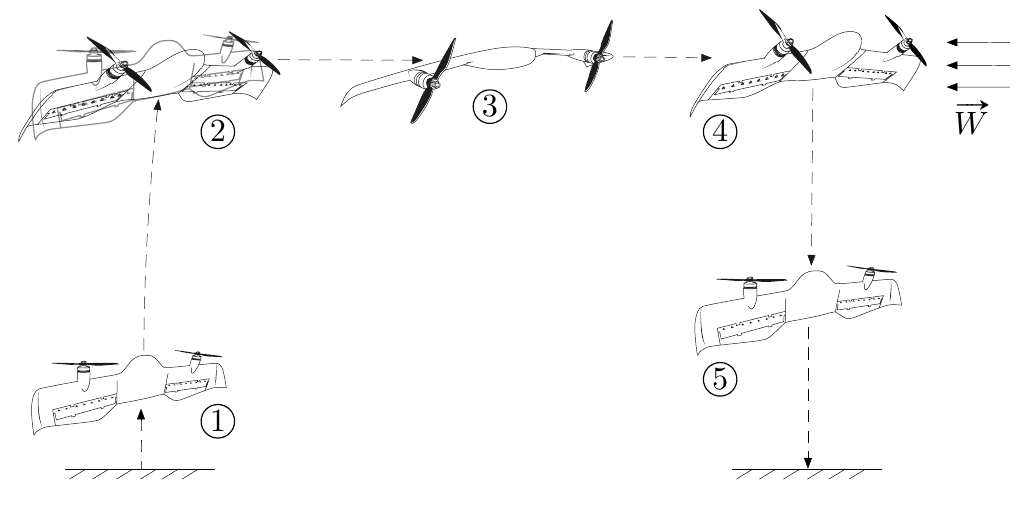
\includegraphics[width=0.8\columnwidth]{figures/darko_transition.png}
        \caption{Phases de vol d'un drone \textit{tailsitters}, DarkO.}
        \label{fig:darko_flight}
\end{figure}

\subsection*{Maquettes}

De nombreuses maquettes réelles ont été assemblées dans le but de réaliser des vols expérimentaux. Citons en exemples le \textit{tailsitter} à double rotor appelé «~T-Wing~» \cite{Stone2002PreliminaryDO, TWing2008}, le \textit{tailsitter} appelé «~MavIon~» \cite{oatao14575}, ou le «~JLion~» et le «~KH-Lion~» \cite{8003167}. Ces trois maquettes sont illustrées sur la figure \ref{fig:maquettetailsitter}.

\begin{figure}[ht!]
    \centering
    \resizebox{.9\textwidth}{!}{%
    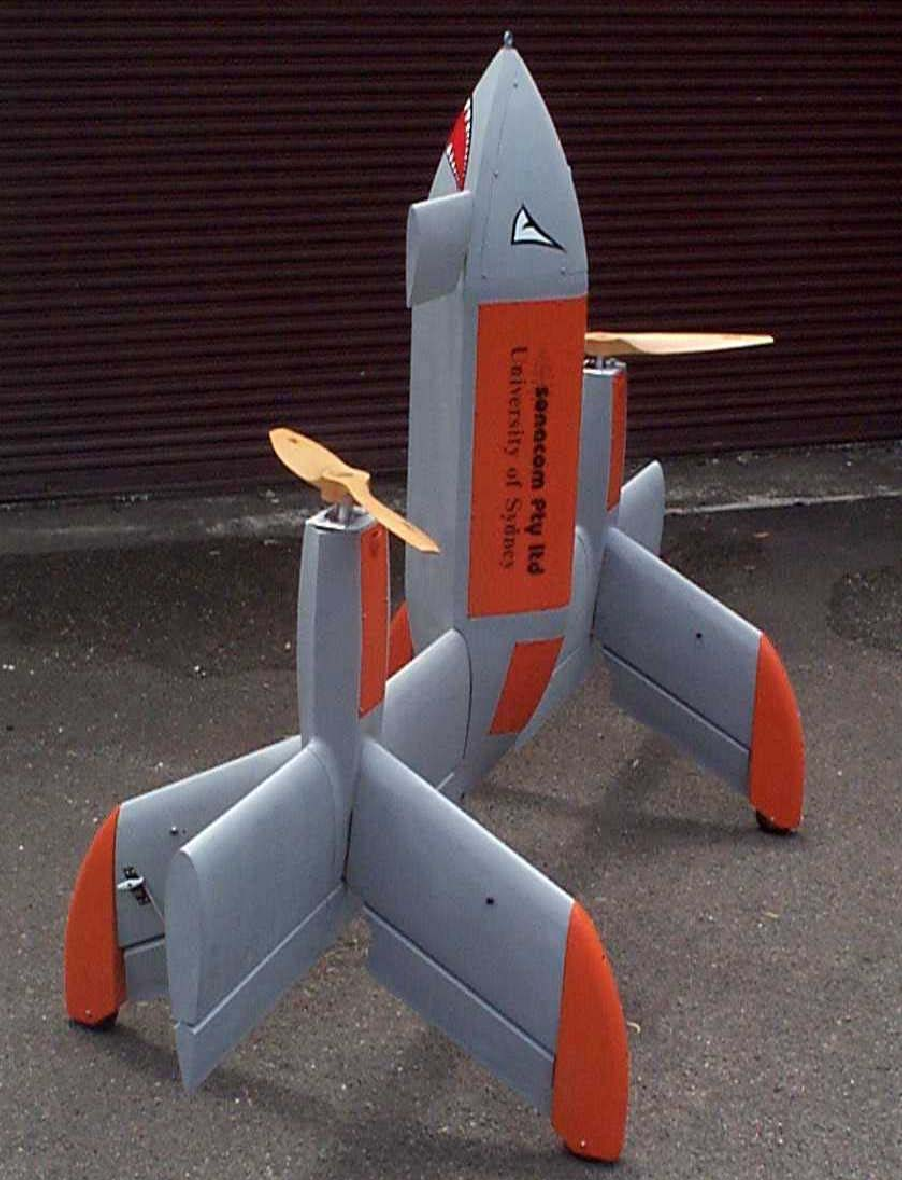
\includegraphics[height=3cm]{figures/T-Wing.png}
    \quad
    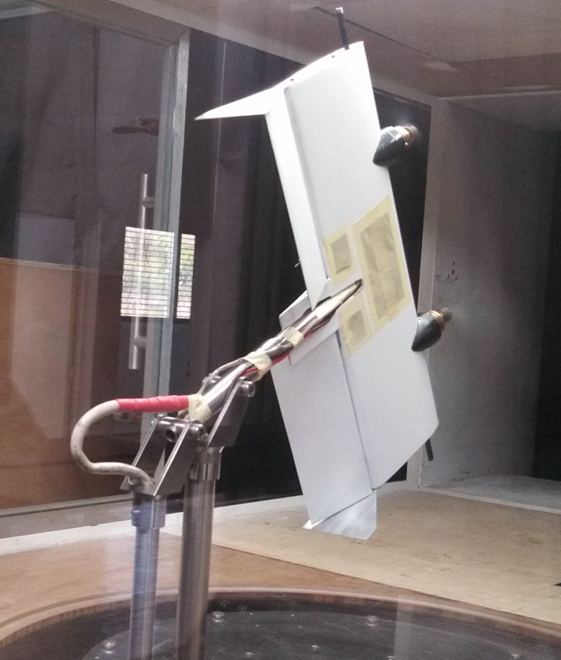
\includegraphics[height=3cm]{figures/mavionWindtunel.png}
    \quad
    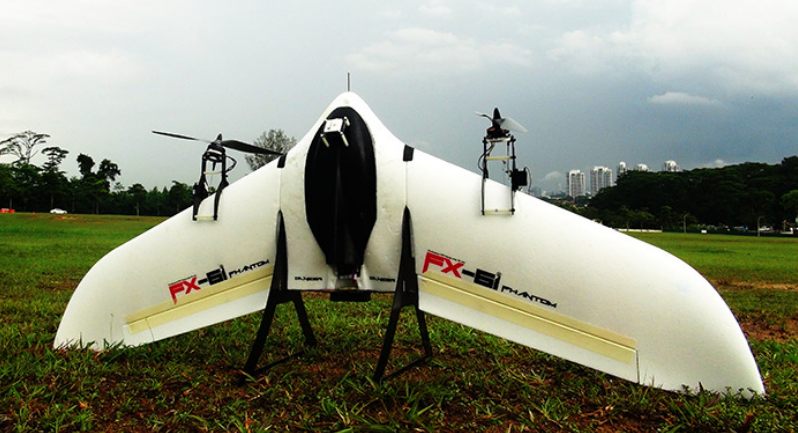
\includegraphics[height=3cm]{figures/KHlion.png}
    }
    \caption{Maquette «~T-Wing~», «~MavIon~» et «~KH-Lion~».}
    \label{fig:maquettetailsitter}
\end{figure}

Ces drones partagent une architecture similaire basée sur une aile supportant deux moteurs sur le bord d'attaque et soufflant deux élevons situés sur le bord de fuite. Cette architecture offre une plus grande robustesse que les \textit{tiltrotors}, composés de pièces mobiles (ce qui les rend plus fragiles) et d'un actionneur puissant pour faire tourner l'ensemble moteur-hélice.
La complexité inhérente à ces architectures nécessite un travail de modélisation en raison des nombreuses non-linéarités et couplages impliqués, en particulier en termes de modélisation des effets aérodynamiques. Dans ce contexte, l'interférence aérodynamique entre l'aile fixe et les rotors a été modélisée dans \cite{droandi_zanotti_gibertini_grassi_campanardi_2015, Simmons2022, aerospace5030079}, et les forces et moments d'hélice générés à des angles d'attaque élevés sont abordés dans \cite{Fernandez2023}. Cependant, ces modèles sont complexes algorithmiquement et ne sont que partiellement utilisables pour la conception des commandes. 

Un autre point important est la représentation de l'attitude du drone. Aussi, il est possible de représenter son orientation par des angles d'Euler \cite{4177650, 5415267, 8003165}, ce qui permet une compréhension intuitive. Toutefois, une singularité apparaît dans certaines phases de vol. Compte tenu de la grande manœuvrabilité, il est préférable de représenter l'attitude par un quaternion unitaire, ce qui élimine toute singularité \cite{8027691}. De nombreuses publications modélisent les effets aérodynamiques générés par les hélices en fonction de l'angle d'attaque et l'angle de dérapage \cite{Escareno07, ChiappinelliNahon2018}. 
Il est possible de choisir un autre modèle pour les interactions aérodynamiques entre les moteurs, les ailes et les élevons, comme présenté dans \cite{lustosaHal-03035938}. La technique de modélisation présentée dans \cite{lustosaHal-03035938} permet de disposer d'un modèle global couvrant l'ensemble de l'enveloppe de vol, grâce à ce que l'on appelle l'approche $\Phi$-théorie. Bien que cette dernière ne permette pas de prédire la chute brutale de la force de portance avec un angle d'attaque croissant (qui est causée par un flux d'air turbulent) \cite{tal2022global}, elle permet de représenter le drone avec suffisamment de précision pour capturer le comportement lors de manœuvres agressives. 



% Actuellement, nous pouvons mentionner deux types d'architectures de commande ayant fonctionné sur ce tailsitter. La première est basée sur une inversion incrémentale non-linéaire de la dynamique du drone (\textit{Incremental Non-linear Dynamic Inversion}, INDI) \nomenclature[]{\(INDI\)}{Inversion incrémentale non-linéaire  (\textit{Incremental Non-linear Dynamic Inversion})} et la seconde est basée sur une technique sans modèle (\textit{Model free control}, MFC). \nomenclature[]{\(MFC\)}{Commande sans modèle (\textit{Model free control})}

Les deux architectures sur lesquelles se sont concentrées nos recherches sont celles de DarkO, un \textit{tailsitters} et de Colibri, un \textit{freewings} basé sur une aile inspirée de DarkO, en rotation libre autour d'un fuselage qui sera maintenu horizontal.


\section*{Question de recherche}

Comme expliqué précédemment, lors des phases de décollage et d'atterrissage, le drone est vertical (voir figure~\ref{fig:darko_flight}), ce qui engendre une grande sensibilité aux perturbations. Il semble pertinent de concentrer nos travaux sur l'étude de la robustesse des drones convertibles face au vent.
Notre travail se focalise sur la recherche d'un contrôleur de vol unifié, pour une architecture de drone fortement non-linéaire et couplée, sur l'intégralité du domaine de vol, en environnement perturbé.

\section*{Objectifs fixés pour la thèse}
Les objectifs fixés sont pluriels : il s'agira d'étudier le comportement d'un drone \textit{tailsitters} en environnement perturbé en présence de saturation des actionneurs pouvant engendrer des cycles limites. Nous utiliserons la linéarisation pour extraire la dynamique du drone autour de l'ensemble des points d'équilibre. Nous étudierons la précision des linéarisations face aux nombreuses non-linéarités du modèle. 

De nos linéarisations, de notre compréhension du fonctionnement du drone et des limites analysées, il s'agira de proposer des architectures de commande basées modèle pour un drone \textit{tailsitters} permettant d'assurer une robustesse aux perturbations de vent. L'intérêt d'une architecture basée modèle est la possibilité de certification de ce type d'architecture. 

Pour finir, nous souhaitons utiliser des capteurs pour mesurer les perturbations en avance de phase pour les rejeter (sonde 5 trous, micro, Pitot, etc.). La connaissance d'une perturbation en amont de son impact sur le drone peut être un point clé dans la diminution de son impact. La mesure associée à un modèle peut être un moyen d'agir en anticipation plutôt qu'en réaction. Une action en anticipation pourrait se traduire par une modification de l'état du drone avant l'arrivée de la perturbation pour en minimiser son impact. À l'inverse qu'une action en réaction est une gestion de la perturbation suite à une modification de l'équilibre du drone (déplacement ou modification de son orientation) qui intervient après que la perturbation ait impacté le drone.  

Au vu des contraintes des \textit{tailsitters}, l'installation de capteurs de mesure de vent implique le développement d'une nouvelle architecture permettant l'installation d'un capteur capable de saisir les perturbations sur l'intégralité du domaine de vol.


\section*{Plan et contribution}
Notre exposé commencera par une description générale des architectures de drone convertible (Chapitre~\ref{chap:generalites}), avec une présentation des avantages et des inconvénients ainsi que leur mode de fonctionnement. Une description générale de la modélisation, de l'actionnement et des lois de commande proposée sur les \textit{tailsitters} et les \textit{freewings} introduira nos propos sur ces architectures.

Le chapitre \ref{chap:model} détaillera le modèle non-linéaire d'un drone \textit{tailsitters}, DarkO, à partir des travaux de \cite{lustosaHal-03035938} et de \cite{olszaneckibarthHal-02542982}. Nous proposons un modèle simplifié pour les basses vitesses, ainsi que le détail des équilibres stationnaires en présence ou non de vent. De ces équilibres, nous présenterons la dynamique linéarisée du drone paramétrée par deux scalaires, le vent horizontal et vertical. Ce modèle étant le point de départ de chacun de nos travaux, il se retrouve expliqué dans \cite[Chapitre 2]{sansouStage} et \cite[Section II]{sansouECC} dans la condition de vent nulle, dans \cite[Section 2]{SANSOUACA} avec des conditions de vent non nulle et dans \cite[Section II]{sansouTCST} sous sa forme la plus complète.

Le chapitre \ref{chap:hybrid} fera l'objet d'une proposition de loi de commande hybride permettant d'augmenter le domaine de stabilité d'une loi linéaire avec une loi de commande non-linéaire basée sur une direction de zéro moment. Ces travaux ont été publiés dans  \cite{sansouStage} et \cite{sansouECC}.

Le chapitre \ref{chap:3DOF} permettra de décrire une maquette expérimentale utilisée pour évaluer les performances d'une loi de commande basée sur une architecture proportionnelle dérivative. Cette loi est un retour de sortie permettant de stabiliser une position stationnaire en présence de vent. Cette maquette restreint les degrés de liberté classiques d'un drone pour se concentrer sur la réjection de perturbation de vent, grâce à un changement d'incidence de la maquette. La description de la loi de commande, son optimisation et les résultats sont disponibles dans \cite{SANSOUACA}.

Le chapitre \ref{chap:LMI} propose une méthode d'obtention des gains de la boucle fermée différente basée sur les inégalités linéaires matricielles et la théorie de Lyapunov. L'ensemble de l'optimisation sera réalisé à l'aide de la dynamique linéarisé du drone autour de la condition de vent nulle. Ce contrôleur sera testé sur une maquette à six degrés de liberté en environnement contrôlé.

Le chapitre \ref{chap:6DOF} étendra le contrôleur proposé dans le chapitre \ref{chap:3DOF} pour stabiliser la dynamique complète d'un drone \textit{tailsitter}. La méthode d'obtention des gains du contrôleur est basée sur un algorithme itératif permettant de maintenir la complexité algorithmique, tout en identifiant les conditions de vol critiques. Les travaux ont été publiés dans \cite{sansouTCST}.

Le chapitre \ref{chap:colibri} propose une nouvelle architecture de \textit{freewing}. Cette dernière est inspirée d'un \textit{tailsitter} sur lequel on adjoint un fuselage pendulaire en rotation libre de manière à le maintenir horizontal dans toutes les configurations de vol. Nos travaux se sont concentrés sur l'obtention d'un modèle de simulation basé sur une dynamique multicorps. Des résultats de simulation et expérimentaux ont été proposés, basés sur un contrôle non-linéaire et publiés dans \cite{sansouICUAS}.





\chapter{Objectifs de commande}
\minitoc
\label{chap:objectif}

\section{Contexte opérationnel}
Tout l'intérêt des drones est leurs capacités à se maintenir stabilisé sans intervention humaine. Ainsi, les opérateurs peuvent se concentrer sur la mission, sans devoir consacrer une grande attention au pilotage du drone. 

Les nombreux progrès dans les systèmes d'estimation état permettent de connaitre précisément l'orientation et la position des drones pour assurer la stabilisation, le guidage et la navigation. Les progrès sont lié à l'amélioration continue des capteurs, notamment des centrales inertielles (Inertial measurement Units, IMU), \nomenclature[]{\(IMU\)}{Centrales inertielles (\textit{Inertial measurement Units})} constitué d'un accéléromètre, d'un gyroscope et d'un magnétomètre. La Table \ref{tab:autopilote_ev} montre l'évolution des vitesses des microcontrôleurs (Microcontroller Unit, MCU) \nomenclature[]{\(MCU\)}{Microcontrôleurs (\textit{Inertial measurement Units})} embarqué sur les autopilotes et de la réduction du bruit des capteurs inertiel.
\begin{table}[ht]
    \centering
    \begin{tabular}{|c|c|c|c|c|c|}
        \hline
        Génération & Année & MCU & Vitesse & Capteur  & Bruit RMS \\
        \hline \hline
        \href{https://wiki.paparazziuav.org/wiki/Apogee/v1.00}{Apogee}  & 2013 & STM32F4 & 168 MHz & MPU-9150 & \begin{tabular}{ccc} Gyro : 0.06 dps \\
        Accel: 4 mg  \end{tabular}  \\
        \hline
        \href{https://wiki.paparazziuav.org/wiki/Chimera/v1.00}{Chimera} & 2016 & STM32F7 & 216 MHz &  MPU-9250 & \begin{tabular}{ccc} Gyro : 0.1  dps \\
        Accel: 8 mg  \end{tabular}\\
        \hline
        \href{https://wiki.paparazziuav.org/wiki/Tawaki/v1.10}{Tawaki 1} &2019 &  STM32F7 & 216 MHz  & ICM-20600 & \begin{tabular}{ccc} Gyro : 0.04 dps \\
        Accel: 1 mg  \end{tabular}\\
        \hline
        \href{https://wiki.paparazziuav.org/wiki/Tawaki/v2.01}{Tawaki 2} &2023 &  STM32H7 & 480 MHz & ICM-42688-P & \begin{tabular}{ccc} Gyro : 0.028 dps \\
        Accel: 0.70 mg  \end{tabular} \\
        \hline
    \end{tabular}
    \caption{Évolution des autopilotes paparazzi sur dix ans.}
    \label{tab:autopilote_ev}
\end{table}

Sur une période de dix ans, nous pouvons observer que les microcontrôleurs ont doublé leurs vitesses d'exécution, que les fabricants ont divisé par deux le bruit moyen sur les gyroscopes et par quatre le bruit moyen des accéléromètres.
Ces évolutions continues permettent une amélioration de l'estimation du drone utilisé pour la stabilisation. Il en résulte une stabilité accrue et de nouvelle possibilité pour la commande des drones.


\section{Contexte de la thèse}
De nombreux travaux ont été mener sur les \textit{tailsitters}, avec l'objectif de couvrir l'intégralité du domaine de vol. Ce dernier est constitué de trois phases, le stationnaire, la transition et le vol d'avancement. Chaque phase possède des contraintes  

vol complet 
methode sans modèles 




\todo{rejet de perturbation, model based control}

\section{Perturbations}

\section{Résumée}
\chapter{Modélisation d'un drone convertible : DarkO}
\minitoc
\label{chap:model}

\section{Modèle du drone DarkO}
\label{sec:model}
DarkO, drone conçu et développé à l'École Nationale de l'Aviation Civile (ENAC) de Toulouse (France), est un exemple clair de drone convertible avec une architecture dite \textit{tailsitter}.
DarkO est assemblé à partir de plusieurs pièces d'Onyx imprimées en 3D (un matériau très robuste composé de fibres de carbone omnidirectionnelles). Toutes les pièces sont emboîtées sur un seul axe, de sorte que le drone puisse facilement être démonté pour remplacer des pièces ou accéder à l'électronique embarquée. 

L'autopilote embarqué est une carte Apogee~\footnote{\url{https://wiki.paparazziuav.org/wiki/Apogee/v1.00}} fabriquée à l'ENAC, voir Fig. \ref{fig:apogee}. 


\begin{figure}[ht!]
    \centering
        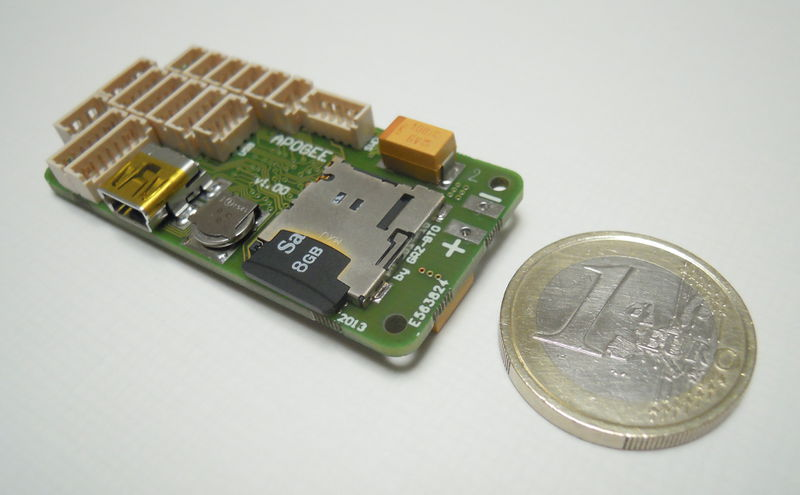
\includegraphics[width=0.8\columnwidth]{figures/800px-Apogee_v100_top_1E.jpeg}
        \caption{Vue de dessus d'un autopilote Apogee v1.00.}
        \label{fig:apogee}
\end{figure}

L'autopilote offre la possibilité d'enregistrer les données de bord sur une carte mémoire SD, à la fréquence de contrôle de 500 Hz, ce qui permet un post-traitement efficace des données acquises. Le protocole de communication utilisé entre l'autopilote et les contrôleurs électroniques de vitesse (ESC) est le Dshot 600. Les ESC sont des AIKON AK32 35A \todo{trouver un synonyme} flasher avec un firmware AM32. La communication sol-bord est réalisée via un canal bidirectionnel basé sur des modules XBee-PRO S1.

\nomenclature[]{\(ESC\)}{Contrôleurs électroniques de vitesse (\textit{Electronic Speed Controller})}



Les actionneurs de DarkO peuvent être décomposés en deux catégories. La première est composée de deux hélices (T-Motor T5147) placées symétriquement à l'avant de l'aile (illustrées en \textbf{noir} dans la Fig. \ref{fig:darko2}) et alimentées par deux moteurs électriques (T-Motor F30 2300kv) générant une traction selon l'axe $x_{b}$. La seconde catégorie est relative aux actionneurs aérodynamiques. Ainsi, le drone possède deux élevons, placés à l'arrière de l'aile (illustrés en \textcolor{cyan}{bleu} dans la Fig. \ref{fig:darko2}), agissant en tant que surfaces de contrôle. Les élevons génèrent des forces et des moments en modifiant leur incidence relativement au flux d'air dans lequel ils sont placés. Ce flux d'air peut être généré par le vent relatif (lié à la vitesse du drone), le vent extérieur, mais aussi par le souffle des hélices. Les élevons sont commandés par deux servomoteurs MKS DS65K.

\begin{figure}[ht!]
    \centering
    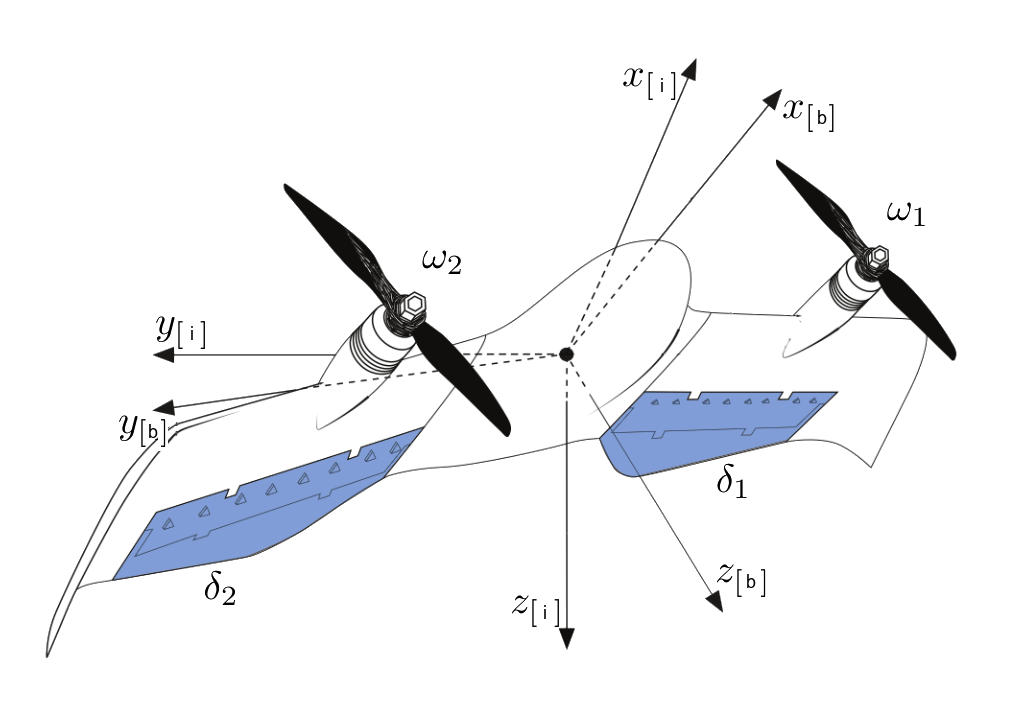
\includegraphics[width=0.8\columnwidth]{figures/darko.png}
    \caption{Repère de référence de DarkO avec une représentation schématique des actionneurs.}
    \label{fig:darko2}
\end{figure}

La figure \ref{fig:darko2} montre le modèle de DarkO, ainsi qu'un repère de référence inertiel \textit{North, east, down} (NED) \nomenclature[]{\(NED\)}{Nord Est Bas (\textit{North, East, Down})} (ou repère terrestre) ``$\text{i}$'' lié à la surface de la Terre, et un repère corps `$\text{b}$'' attaché au drone, avec $x_{\text{b}}$ correspondant à l'axe de roulis (l'axe des hélices dans le plan $z_{ \text{b} } = 0$), $y_{\text{b}}$ l'axe de tangage (la direction des ailes), $z_{\text{b}}$ l'axe de lacet. En utilisant la même notation que dans \cite{lustosaHal-03035938}, le couple hélice/élévateur gauche et droit sont désignés par les indices $i=1$ (gauche) et $i=2$ (droite). La convention de signe sera définie comme positive pour les positions des élevons $\delta_{1}$, $\delta_{2}$ lorsqu'ils créent un moment à cabrer avec les hélices tournant dans des directions opposées avec des vitesses angulaires $\omega_{1} > 0$ et $\omega_{2} < 0$, respectivement.

\begin{table}[ht]
    \centering
      \begin{tabular}{|l|c|c|}
        \hline
        \multicolumn{1}{|c|}{Paramètres et coefficients} & Valeurs & Unités \\
        \hline
        $m$ (Masse du drone)  & 0.519 & \SI{}{\kilogram} \\
        \hline
        $b$ (Envergure)  & 0.542 & \SI{}{\meter} \\
        \hline
        $c$ (Corde aérodynamique)  & 0.13 & \SI{}{\meter} \\
        \hline
        $\boldsymbol{B}=\diag(b,c,b)$ & $\!\!\diag(0.542, 0.13, 0.542)$ \!\! & \SI{}{\meter}\\
        \hline
        $S$ (Surface de l'aile) & 0.026936 & \SI{}{\square\meter}\\
        \hline
        $S_{\text{wet}}$ (Surface soufflée) & 0.0180 & \SI{}{\square\meter}\\
        \hline
        $S_{\text{p}}$ (Surface des hélices) & 0.0127 & \SI{}{\square\meter}\\
        \hline
        $\boldsymbol{J}=\diag(J_{x},J_{y},J_{z})$ & \!\! $\diag(0.0067,0.0012,0.0082)$\!\! & \SI{}{\kilogram\square\meter}\\
        \hline
        $k_{\text{f}}$ (Poussée des hélices) & 1.7800e-8 & \SI{}{\kilogram\meter}\\
        \hline
        $k_{\text{m}}$(Moment des hélices) & 2.1065e-10 & \SI{}{\kilogram\square\meter}\\
        \hline
        $p_{x}$ (Position en $x$ des hélices) & 0.065 & \SI{}{\meter}\\
        \hline
        $p_{y}$ (Position en $y$  des hélices) & 0.162 & \SI{}{\meter}\\
        \hline
        $a_{y}$ (Position en $y$ de la portance) & 0.1504 & \SI{}{\meter}\\
        \hline
        $\xi_{\text{f}}$ (Portance des élevons) & 0.2 & --\\
        \hline
        $\xi_{\text{m}}$ (Moment des élevons) & 1.4 & --\\
        \hline
        $\rho$ (Densité de l'air) & 1.225 & \SI{}{\kilogram\per\cubic\meter}\\
        \hline
        $C_{\text{d}}$ (Trainé) & 0.1644 & --\\
        \hline
        $C_{y}$ (Latéral) & 0 & --\\
        \hline
         $C_{\ell}$ (Portance) & 5.4001 & --\\
        \hline
        $\Delta_{\text{r}}$ (Centrage du drone) & -0.0145 & \SI{}{\meter}\\
        \hline
      \end{tabular}
      \caption{Paramètres numériques identifiés du modèle DarkO.}
      \label{tab:pars}
\end{table}

\subsection{Modèle non-linéaire complet}

En exploitant la modélisation présentée dans \cite{lustosaHal-03035938} et \cite{olszaneckibarthHal-02542982}, un modèle précis de la dynamique de DarkO décrit la position $\boldsymbol{p} \in \real^3$ du centre de gravité et sa vitesse $\boldsymbol{v} = \dot{\boldsymbol{p}} \in \real^3$, son orientation, bien représentée par un quaternion $\boldsymbol{q} \in {\mathbb S}^3:=\{ \boldsymbol{q} \in \real^4 : |\boldsymbol{q}| = 1\}$, et de sa vitesse angulaire $\boldsymbol{\omega}_{\text{b}}$, représentée dans le repère du corps, qui satisfait $\boldsymbol{\dot q} = \frac{1}{2}\boldsymbol{q} \otimes \smallmat{0 \\ \boldsymbol{\omega}_{{\text{b}}}}$, où $\otimes$ représente le produit hamiltonien (voir \cite{lustosaHal-03035938,olszaneckibarthHal-02542982} ou le tutoriel \cite{hamel_minhduc} pour plus de détails).
\todo{produit hamiltonien}
En choisissant l'état global comme $\boldsymbol{x}:=(\boldsymbol{p},~ \boldsymbol{v},~ \boldsymbol{q},~ \boldsymbol{\omega}_{\text{b}})$, le modèle mathématique, dérivé dans \cite{lustosaHal-03035938}, dépend d'un ensemble de paramètres énumérés dans le tableau \ref{tab:pars}, où nous indiquons également la valeur obtenue à partir d'une identification du système \cite{sansouStage}. Le modèle dynamique peut être écrit comme ci-dessous :

\begin{subequations}\label{eq:dyna_orig}
    \begin{empheq}[left=\empheqlbrace]{alignat=2}
           \boldsymbol{\dot p} & &= & \boldsymbol{v} \label{eq:dyna_orig_a}\\
          \label{eq:dyna_orig_b}
          m\boldsymbol{\dot v} &&=& - m\boldsymbol{g} +  \boldsymbol{R}(\boldsymbol{q})\boldsymbol{F}_{\text{b}},\\
          \boldsymbol{\dot q} &&=& \frac{1}{2}\boldsymbol{q} \otimes \boldsymbol{\omega_{b}} \label{eq:dyna_orig_c}\\
          \label{eq:dyna_orig_d}
          \boldsymbol{J} \boldsymbol{\dot \omega_{\text{b}}} &&= &  - \skewsym{\boldsymbol{\omega}_{\text{b}}}\boldsymbol{J}\boldsymbol{\omega}_{\text{b}} + \boldsymbol{M}_{\text{b}},
    \end{empheq}
  \end{subequations}
  où $\boldsymbol{g}:=\smallmat{0 & 0& 9.81}^\top$ désigne le vecteur de gravité, $m\in \real$ est la masse, $\boldsymbol{J}\in \real^{3\times 3}$ est le moment d'inertie diagonal (voir Tableau~\ref{tab:pars}) et en partitionnant le quaternion $\boldsymbol{q} \in {\mathbb S}^3$ comme $\boldsymbol{q} := \left[ \eta ~ \boldsymbol{\epsilon}^\top \right]^\top$, la matrice de rotation correspondante est $\boldsymbol{R}(\boldsymbol{q}) \in SO(3): = \{\boldsymbol{R}\in \real^{3\times 3}: \; \boldsymbol{R}^\top \boldsymbol{R} = \mathbb{I}_{3}, \det (\boldsymbol{R})=1\}$ est défini comme (voir \cite{hamel_minhduc})
\begin{align}
    \label{eq:matrix_rot}
    \boldsymbol{R}(\boldsymbol{q}) := \mathbb{I}_{3} +2\eta \skewsym{\boldsymbol{\epsilon}} + 2\skewsym{\boldsymbol{\epsilon}}^{2}.
\end{align}


D'après \cite{lustosaHal-03035938}, le vecteur de force $\boldsymbol{F}_{\text{b}}$ et le vecteur de moment $\boldsymbol{M}_{\text{b}}$ dans \eqref{eq:dyna_orig} dépendent  (i) de l'état du système $\boldsymbol{x}$, (ii) de la perturbation $\boldsymbol{w} \in \real^3$, représentant la vitesse du vent dans le référentiel inertiel, et (iii) de la commande des actionneurs (voir Figure~\ref{fig:darko2}), comprenant la vitesse de rotation des deux hélices $\omega_1, \omega_2 \in \real$ et la déflexion des élevons $\delta_1, \delta_2\in \real$.
Considérons d'abord l'effet des commandes des actionneurs. Chaque hélice génère une poussée $\boldsymbol{T}_i$ orientée dans la direction $x$ du repère corps et un moment $\boldsymbol{N}_i$ selon le même axe :
\begin{align}
\label{eq:thrust}
\boldsymbol{T}_{i} \!:=\! \begin{bmatrix} \tau_{i} \\ 0 \\ 0 \end{bmatrix} \!:=\!
\begin{bmatrix} k_{\text{f}}\omega_{i}^{2} \\ 0 \\ 0 \end{bmatrix}\! , \;
\boldsymbol{N}_{i} \!:=\! (-1)^{i}  \frac{k_{\text{m}} }{k_{\text{f}}}\boldsymbol{T}_{i}, \quad i=1,2 .
\end{align} 

La position de chaque élevon $\delta_i \in \real$ est assignée par un servomoteur qui impose un niveau d'efficacité (en termes de déviation du courant d'air) quantifié par deux matrices antisymétriques :
\begin{align}
\label{eq:elevons_efficiency}
    \boldsymbol{\Delta}^{\text{f}}_{i} \!:=\! \begin{bmatrix} 0 & 0 & \xi_{\text{f}}\delta_{i} \\ 0 & 0 & 0 \\ -\xi_{\text{f}}\delta_{i} & 0 & 0 \end{bmatrix}\! ,\;
    \boldsymbol{\Delta}^{\text{m}}_{i} \!:=\! \begin{bmatrix} 0 & 0 & \xi_{\text{m}}\delta_{i} \\ 0 & 0 & 0 \\ -\xi_{\text{m}}\delta_{i} & 0 & 0 \end{bmatrix} \!, \quad i=1,2.
\end{align}
 Les paramètres constants $k_{\text{f}}$, $k_{\text{m}}$, $\xi_{\text{f}}$, $\xi_{\text{m}}$ apparaissant dans \eqref{eq:thrust} et \eqref{eq:elevons_efficiency} sont listés dans la Table~\ref{tab:pars}.\\
Avec les quantités ci-dessus, nous pouvons réarranger la dynamique donnée dans le tableau suivant \cite[eqns (97),~(98)]{lustosaHal-03035938} (voir aussi \cite{sansouStage}) et exprimer $\boldsymbol{F}_{\text{b}}$ et $\boldsymbol{M}_{\text{b}}$ dans \eqref{eq:dyna_orig} comme
%
\begin{align}
\nonumber
    \boldsymbol{F}_{\text{b}} :={}&  \boldsymbol{T}_{1} + \boldsymbol{T}_{2} + \frac{S_{\text{wet}}}{4S_{\text{p}}} \boldsymbol{\Phi}^{\text{(fv)}} \Big( (\boldsymbol{\Delta}^{\text{f}}_1 - \mathbb{I}_{3} ) \boldsymbol{T}_{1} + ( \boldsymbol{\Delta}^{\text{f}}_2 - \mathbb{I}_{3}) \boldsymbol{T}_{2}\Big) \\ 
     \label{eq:Fb}
    &+ \frac{1}{4} \rho S  \boldsymbol{\Phi}^{\text{(fv)}} \Big(\boldsymbol{\Delta}^{\text{f}}_1+ \boldsymbol{\Delta}^{\text{f}}_2 - 2 \mathbb{I}_{3} \Big) \lVert \boldsymbol{v_{\text{b}}} \rVert \boldsymbol{v_{\text{b}}}\\
    \nonumber
    &+ \frac{1}{4} \rho S \boldsymbol{\Phi}^{\text{(mv)}} \Big(\boldsymbol{\Delta}^{\text{f}}_1 + \boldsymbol{\Delta}^{\text{f}}_2 - 2\mathbb{I}_{3}\Big) \boldsymbol{B} \lVert \boldsymbol{v_{\text{b}}} \rVert  \boldsymbol{\omega}_{\text{b}}, 
\end{align}
\begin{align} 
\label{eq:Mb}
 \boldsymbol{M}_{\text{b}} :&=\boldsymbol{N}_{1} + \boldsymbol{N}_{2} + \skewsym{\smallm{p_x\\ p_y\\ 0}} \boldsymbol{T}_{1} + \skewsym{\smallm{p_x\\ - p_y\\ 0}} \boldsymbol{T}_{2}\\
    \nonumber
  &- \frac{S_{\text{wet}}}{4S_{\text{p}}} \bigg( \boldsymbol{B} \boldsymbol{\Phi}^{\text{(mv)}} (\boldsymbol{\Delta}^{\text{m}}_1- \mathbb{I}_{3} ) + \skewsym{\smallm{0 \\ a_y \\ 0}} \boldsymbol{\Phi}^{\text{(fv)}} (\boldsymbol{\Delta}^{\text{m}}_1 +\mathbb{I}_{3} ) \bigg) \boldsymbol{T}_{1} \\
    \nonumber
  & - \frac{S_{\text{wet}}}{4S_{\text{p}}} \bigg( \boldsymbol{B} \boldsymbol{\Phi}^{\text{(mv)}} (\boldsymbol{\Delta}^{\text{m}}_2 - \mathbb{I}_{3} ) +  \skewsym{\smallm{0 \\ - a_y \\ 0}} \boldsymbol{\Phi}^{\text{(fv)}} (\boldsymbol{\Delta}^{\text{m}}_2 + \mathbb{I}_{3}) \bigg) \boldsymbol{T}_{2} \\
    \nonumber
  & + \frac{1}{4} \rho S  \bigg( \Big(\skewsym{\smallm{0 \\ a_y \\ 0}} \!\!\! \boldsymbol{\Phi}^{\text{(fv)}}  + \boldsymbol{B} \boldsymbol{\Phi}^{\text{(mv)}} \Big) \boldsymbol{\Delta}^{\text{m}}_1 \\
    \nonumber
  &  + \Big( \skewsym{\smallm{0 \\ - a_y \\ 0}} \!\!\! \boldsymbol{\Phi}^{\text{(fv)}} + \boldsymbol{B} \boldsymbol{\Phi}^{\text{(mv)}}  \Big) \boldsymbol{\Delta}^{\text{m}}_2 - 2 \boldsymbol{B} \boldsymbol{\Phi}^{\text{(mv)}}  \bigg) \lVert \boldsymbol{v_{\text{b}}} \rVert \boldsymbol{v_{\text{b}}} \\
    \nonumber
  & +\frac{1}{4} \rho S \bigg(\!\! \Big(\!\! \skewsym{\!\smallm{0 \\ a_y \\ 0}\!}\!\!\! \boldsymbol{\Phi}^{\text{(mv)}} \! + \! \boldsymbol{B} \boldsymbol{\Phi}^{\text{(m$\omega$)}} \Big) \boldsymbol{\Delta}^{\text{m}}_1 \\
    \nonumber
  & +  \Big(\!\! \skewsym{\!\smallm{0 \\ - a_y \\ 0}\!} \!\!\! \boldsymbol{\Phi}^{\text{(mv)}} \! + \! \boldsymbol{B} \boldsymbol{\Phi}^{\text{(m$\omega$)}}  \Big) \boldsymbol{\Delta}^{\text{m}}_2 - 2 \boldsymbol{B} \boldsymbol{\Phi}^{\text{(m$\omega$)}}\!  \bigg)\!  \boldsymbol{B}  \lVert \boldsymbol{v_{\text{b}}} \rVert  \boldsymbol{\omega}_{\text{b}} ,
\end{align}
où $\boldsymbol{v}_{\text{b}} := \boldsymbol{R}^\top(\boldsymbol{q}) (\boldsymbol{v}-\boldsymbol{w})$ représente la vitesse de l'air vu par le drone exprimé dans le repère du corps. Dans \cite{lustosaHal-03035938}, la valeur $\lVert \boldsymbol{v_{\text{b}}} \rVert$ apparaissant dans les expressions de  $\boldsymbol{F}_{\text{b}}$ et $\boldsymbol{M}_{\text{b}}$ est remplacé par la valeur $\eta = \sqrt{\lVert \boldsymbol{v_{\text{b}}} \rVert^{2} + \mu c^{2} \lVert \boldsymbol{\omega}_{\text{b}} \rVert^{2}}$, avec $\mu \in \real$ étant un paramètre lié à l'identification du modèle. Toutefois, dans le cas de DarkO, l'identification fournit $\mu = 0$ \cite{sansouStage}. Ainsi, nous présentons ici une description simplifiée. La matrice des coefficients aérodynamiques constants 
$\boldsymbol{\Phi}:= \begin{bmatrix} \boldsymbol{\Phi}^{\text{(fv)}} & {\boldsymbol{\Phi}^{\text{(mv)}}}^\top \\ \boldsymbol{\Phi}^{\text{(mv)}} & \boldsymbol{\Phi}^{\text{(m$\omega$)}} \end{bmatrix} \in \real^{6 \times 6}$, est défini dans \cite[eqs. (6)--(9)]{olszaneckibarthHal-02542982} comme $ \boldsymbol{\Phi}^{\text{(fv)}} \!:=\! \diag(C_{\text{d}},C_{y}, C_{\ell})$ et
\begin{align*}
&\left[ \begin{array}{c|c}
    \boldsymbol{\Phi}^{\text{(mv)}}  &  \boldsymbol{\Phi}^{\text{(m$\omega$)}} 
\end{array}\right] :=\\ 
&\left[ \begin{array}{ccc|ccc}
    0 & 0 & 0    &                                          0.1396 & 0 & 0.0573 \\
    0 & 0 & \!\!\!\!\! -\frac{\Delta_{\text{r}}}{c}C_{\ell} &    0 &  0.6358  & 0 \\
    0 & 0 & 0 &     0.0405 & 0 & 0.0019 
\end{array}\right],
\end{align*}
les valeurs numériques des constantes figurant dans le tableau \ref{tab:pars} (ces valeurs numériques n'ont pas été indiquées dans \cite{lustosaHal-03035938} et \cite{olszaneckibarthHal-02542982} et sont données ici pour permettre de reproduire les résultats de nos simulations). 


\subsection{Modèle non linéaire simplifiée à basse vitesse}
\label{sec:model_NL_simp}

Dans la mesure où nous allons nous intéresser au maintien du drone en stationnaire, c'est-à-dire avec une vitesse du drone faible, nous pouvons simplifier la dynamique \eqref{eq:dyna_orig} en négligeant les effets aérodynamiques quadratiques dûs à la vitesse $\boldsymbol{v_{\text{b}}}$ et à la vitesse angulaire $\boldsymbol{\omega}_{\text{b}}$ dans \eqref{eq:Fb} et \eqref{eq:Mb}. 
Nous définissons le vecteur de commande :
\begin{align}
\label{eq:vector_u}
    \boldsymbol{u} := \begin{bmatrix}\tau_{1}  \!&\! \tau_{2}  \!&\! \delta_{1} \!&\! \delta_{2} \end{bmatrix}^\top,
\end{align}
lequel permet d'obtenir le modèle basse vitesse comportant les effets majeurs non-linéaires du vent :
\begin{subequations}\label{eq:dyna_simp}
    \begin{alignat}{3}
    &\boldsymbol{\dot p} = \boldsymbol{v}, \label{eq:dyna1}\\
       & m\boldsymbol{\dot v} =\! \shortminus m\boldsymbol{g} \!+ \! \boldsymbol{R} (\boldsymbol{q}) \!\!\left( \! \boldsymbol{M}_{\text{f}}(\boldsymbol{u}) \! + \! \boldsymbol{D}_{\text{f}}(\boldsymbol{u}) \| \boldsymbol{w} \| \boldsymbol{R}^\top \!(\boldsymbol{q}) (\boldsymbol{v} \! \shortminus \! \boldsymbol{w}) \! \right)\!,\!\! \label{eq:dyna2}\\
        &\boldsymbol{\dot q} = \frac{1}{2}\boldsymbol{q} \otimes \smallmat{0 \\ \boldsymbol{\omega}_{\text{b}}}, \label{eq:dyna3}\\
        &\boldsymbol{J} \boldsymbol{\dot \omega}_{\text{b}} = \shortminus \skewsym{\boldsymbol{\omega}_{\text{b}}}\boldsymbol{J}\boldsymbol{\omega}_{\text{b}}\! + \boldsymbol{M}_{\text{m}}(\boldsymbol{u})\! + \boldsymbol{D}_{\text{m}} (\boldsymbol{u}) \lVert \boldsymbol{w} \rVert \boldsymbol{R}^\top(\boldsymbol{q}) (\boldsymbol{v}-\boldsymbol{w}), \label{eq:dyna4}
    \end{alignat}
\end{subequations}
où les vecteurs $\boldsymbol{M}_{\text{f}}(\boldsymbol{u})$ et $ \boldsymbol{M}_{\text{m}}(\boldsymbol{u})$, et les matrices $\boldsymbol{D}_{\text{f}}(\boldsymbol{u})$ et $\boldsymbol{D}_{\text{m}} (\boldsymbol{u})$ proviennent de l'annulation des termes dépendant de la vitesse angulaire dans l'équation \eqref{eq:Fb} et \eqref{eq:Mb}. Ils peuvent être développés en 
\begin{align}
\label{eq:Mf}
    \boldsymbol{M}_{\text{f}}(\boldsymbol{u}) :&=  \boldsymbol{T}_{1} \!+\! \boldsymbol{T}_{2} \!+\! \frac{S_{\text{wet}}}{4S_{\text{p}}} \boldsymbol{\Phi}^{\text{(fv)}} \Big( (\boldsymbol{\Delta}^{\text{f}}_1 \shortminus \mathbb{I}_{3} ) \boldsymbol{T}_{1} + ( \boldsymbol{\Delta}^{\text{f}}_2 \shortminus \mathbb{I}_{3}) \boldsymbol{T}_{2}\Big) \nonumber\\
     &=\begin{bmatrix} \left(1-\frac{S_{\text{wet}}}{4S_{\text{p}}} C_{\text{d}}\right) (\tau_{1} + \tau_{2}) \\  0  \\ -\frac{S_{\text{wet}}}{4S_{\text{p}}}C_{\ell}\xi_{\text{f}} \left(\delta_{1}\tau_{1} + \delta_{2}\tau_{2}\right) \end{bmatrix},
\end{align}
\begin{align}
\nonumber
 \boldsymbol{M}_{\text{m}}(\boldsymbol{u}) :&= \boldsymbol{N}_{1} + \boldsymbol{N}_{2} + \skewsym{\smallm{p_x\\ p_y\\ 0}} \boldsymbol{T}_{1} + \skewsym{\smallm{p_x\\ -p_y\\ 0}} \boldsymbol{T}_{2}\\
 \nonumber
   &\quad \shortminus \frac{S_{\text{wet}}}{4S_{\text{p}}}\! \bigg( \boldsymbol{B} \boldsymbol{\Phi}^{\text{(mv)}} (\boldsymbol{\Delta}^{\text{m}}_1- \mathbb{I}_{3} ) \! + \! \skewsym{\smallm{0 \\ a_y \\ 0}} \!\! \boldsymbol{\Phi}^{\text{(fv)}} (\mathbb{I}_{3} + \boldsymbol{\Delta}^{\text{m}}_1 ) \bigg) \boldsymbol{T}_{1} \\
   \nonumber
   &\quad \shortminus \frac{S_{\text{wet}}}{4S_{\text{p}}} \!\bigg( \boldsymbol{B} \boldsymbol{\Phi}^{\text{(mv)}} (\boldsymbol{\Delta}^{\text{m}}_2 - \mathbb{I}_{3} ) \! + \! \skewsym{\smallm{0 \\ \!\shortminus a_y \!\\ 0}} \!\! \boldsymbol{\Phi}^{\text{(fv)}} (\mathbb{I}_{3} + \boldsymbol{\Delta}^{\text{m}}_2 ) \bigg) \boldsymbol{T}_{2} \\
   \label{eq:Mm}
    &=\begin{bmatrix} \frac{k_{\text{m}} }{k_{\text{f}}}(\tau_{1} - \tau_{2}) + \frac{S_{\text{wet}}}{4S_{\text{p}}}a_{y}C_{\ell}\xi_{\text{f}}(\delta_{1}\tau_{1} - \delta_{2}\tau_{2}) \\
   \frac{S_{\text{wet}}}{4S_{\text{p}}} \Delta_{\text{r}}C_{\ell}\xi_{\text{m}}(\delta_{1}\tau_{1} + \delta_{2}\tau_{2}) \\
   \left(p_{y}+\frac{S_{\text{wet}}}{4S_{\text{p}}} a_{y} C_{\text{d}}\right)(\tau_{1} - \tau_{2})
   \end{bmatrix},
\end{align}
\begin{align}
    \boldsymbol{D}_{\text{f}}(\boldsymbol{u}) :&=  \frac{1}{4} \rho S  \boldsymbol{\Phi}^{\text{(fv)}} \Big( \boldsymbol{\Delta}^{\text{f}}_1+  \boldsymbol{\Delta}^{\text{f}}_2 - 2 \mathbb{I}_{3} \Big)   \nonumber \\
 &= \frac{1}{4}\rho S  \begin{bmatrix}
       -2C_{\text{d}} & 0 & C_{\text{d}}\xi_{\text{f}}(\delta_{1} +\delta_{2})\\
       0 & 0 & 0\\
       -C_{\ell}\xi_{\text{f}}(\delta_{1} +\delta_{2}) & 0 & -2C_{\ell}
   \end{bmatrix}, \label{eq:df}
\end{align}
\begin{align}
    \nonumber
    \boldsymbol{D}_{\text{m}}(\boldsymbol{u}) :&= \frac{1}{4} \rho S  \bigg( \Big(\skewsym{\smallm{0 \\ a_y \\ 0}} \!\!\!  \boldsymbol{\Phi}^{\text{(fv)}}  +  \boldsymbol{B}  \boldsymbol{\Phi}^{\text{(mv)}} \Big)  \boldsymbol{\Delta}^{\text{m}}_1  \\
     &\quad  + \Big( \skewsym{\smallm{0 \\ -a_y \\ 0}} \!\!\!  \boldsymbol{\Phi}^{\text{(fv)}} +  \boldsymbol{B}  \boldsymbol{\Phi}^{\text{(mv)}}  \Big)  \boldsymbol{\Delta}^{\text{m}}_2 - 2  \boldsymbol{B}  \boldsymbol{\Phi}^{\text{(mv)}}  \bigg) \nonumber \\
     &= \frac{1}{4}\rho S  \begin{bmatrix}
              \shortminus a_{y}C_{\text{d}}\xi_{\text{m}}(\delta_{1} \!-\! \delta_{2}) \!\! & 0 & 0\\
              \Delta_{\text{r}}C_{\ell}\xi_{\text{m}}(\delta_{1} +\delta_{2})\!\! & 0 & 2\Delta_{\text{r}}C_{\ell}\\
             0 & 0 & \!\! \shortminus a_{y}C_{\ell}\xi_{\text{m}}(\delta_{1} \!-\!\delta_{2})
          \end{bmatrix},   \label{eq:dm}  
\end{align}
où l'on observe l'effet non linéaire d'un vent non nul, qui est non linéaire avec $\boldsymbol{q}$, $\lVert \boldsymbol{v}_{\text{b}} \rVert$ et $\boldsymbol{w}$. Comme dans \cite[eqn. (10)]{olszaneckibarthHal-02542982} et selon la formule de Diederich, nous obtenons $C_{\ell} = C_{\text{d}} + \frac{\pi AR}{1+\sqrt{1+\left(\frac{AR}{2}\right)^{2}}}$ où $AR = \frac{b^{2}}{S}$ est l'allongement de l'aile.
Nous observons le couplage des actionneurs $\left(\delta_{1}\tau_{1} + \delta_{2}\tau_{2}\right)$  dans les expressions des matrices $\boldsymbol{M}_{\text{f}}(\boldsymbol{u})$ et $\boldsymbol{M}_{\text{m}}(\boldsymbol{u})$.

\section{Identification des paramètres du modèle}
    Les valeurs numériques du tableau \ref{tab:pars} ont été obtenues par une campagne d'identification du modèle \cite{sansouStage}. En particulier, le coefficient $k_{\text{f}}$ a été identifié à partir de l'équation \eqref{eq:thrust}, qui relie la vitesse de rotation du moteur $\omega_{i}$ à la traction générée, à la vitesse de rotation minimale et maximale et à la constante de temps de la chaîne d'actionnement du moteur.
    \begin{figure}[ht!]
        \centerline{
        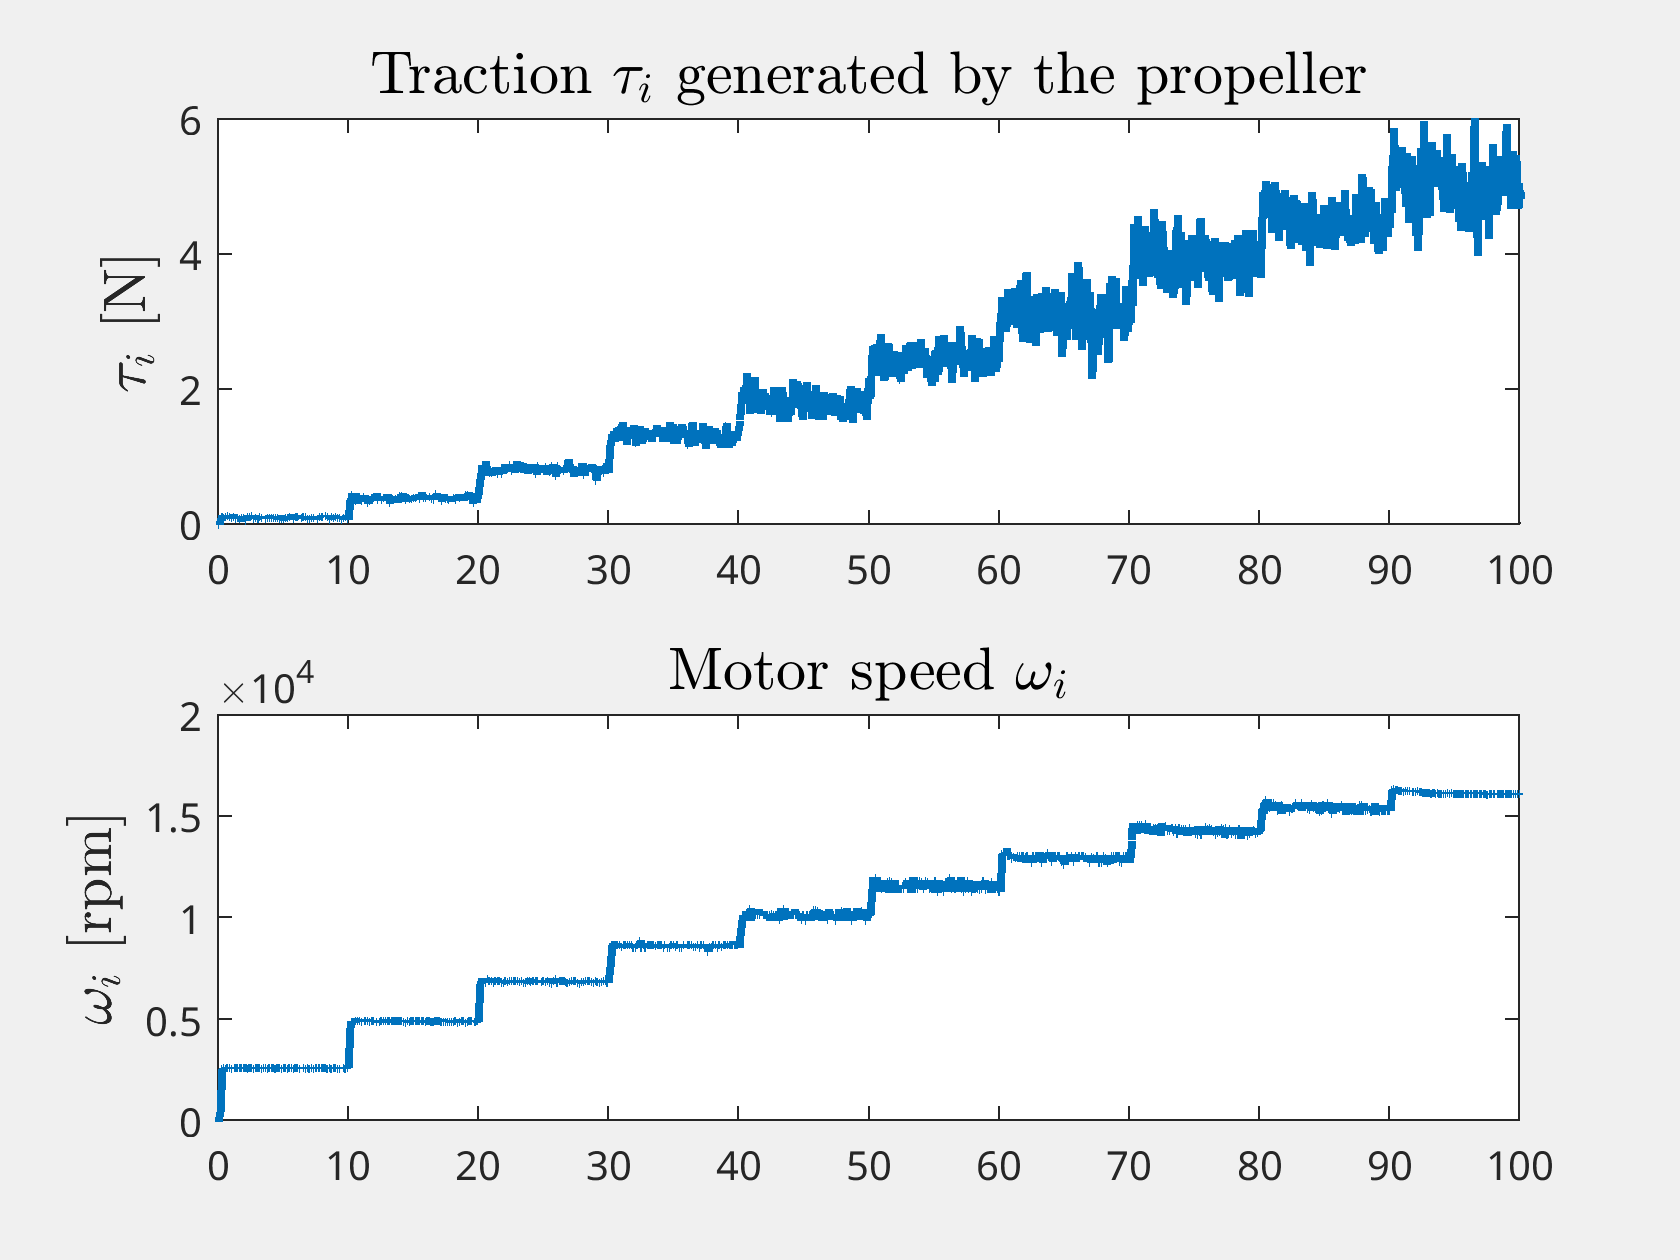
\includegraphics[trim=0cm 0cm 0cm 0cm,clip,width=0.5\columnwidth]{figures/ident_motor March 27 2024 1651.png}}
        \caption{Réponse entrée-sortie de l'ensemble moteur/hélice.}
        \label{fig:IOmot}
    \end{figure}
    
    Pour effectuer, l'identification des 3 coefficients principaux (diagonaux) de la matrice d'inertie, nous avons réalisé un montage d'un système de pendule bifilaire. Cette méthode est largement utilisée dans le domaine des drones \cite{Jardin2007OptimizedMO}, et est basée sur la période d'oscillation autour de chacun des trois axes ($x_{{\text{b}}}$, $y_{\text{b}}$, $z_{\text{b}}$) du drone, lequel est suspendu par deux fils, ce qui forme un pendule de torsion comme le montre la Fig. \ref{fig:BifilarPend}.

    \begin{figure}[ht!]
        \centerline{
        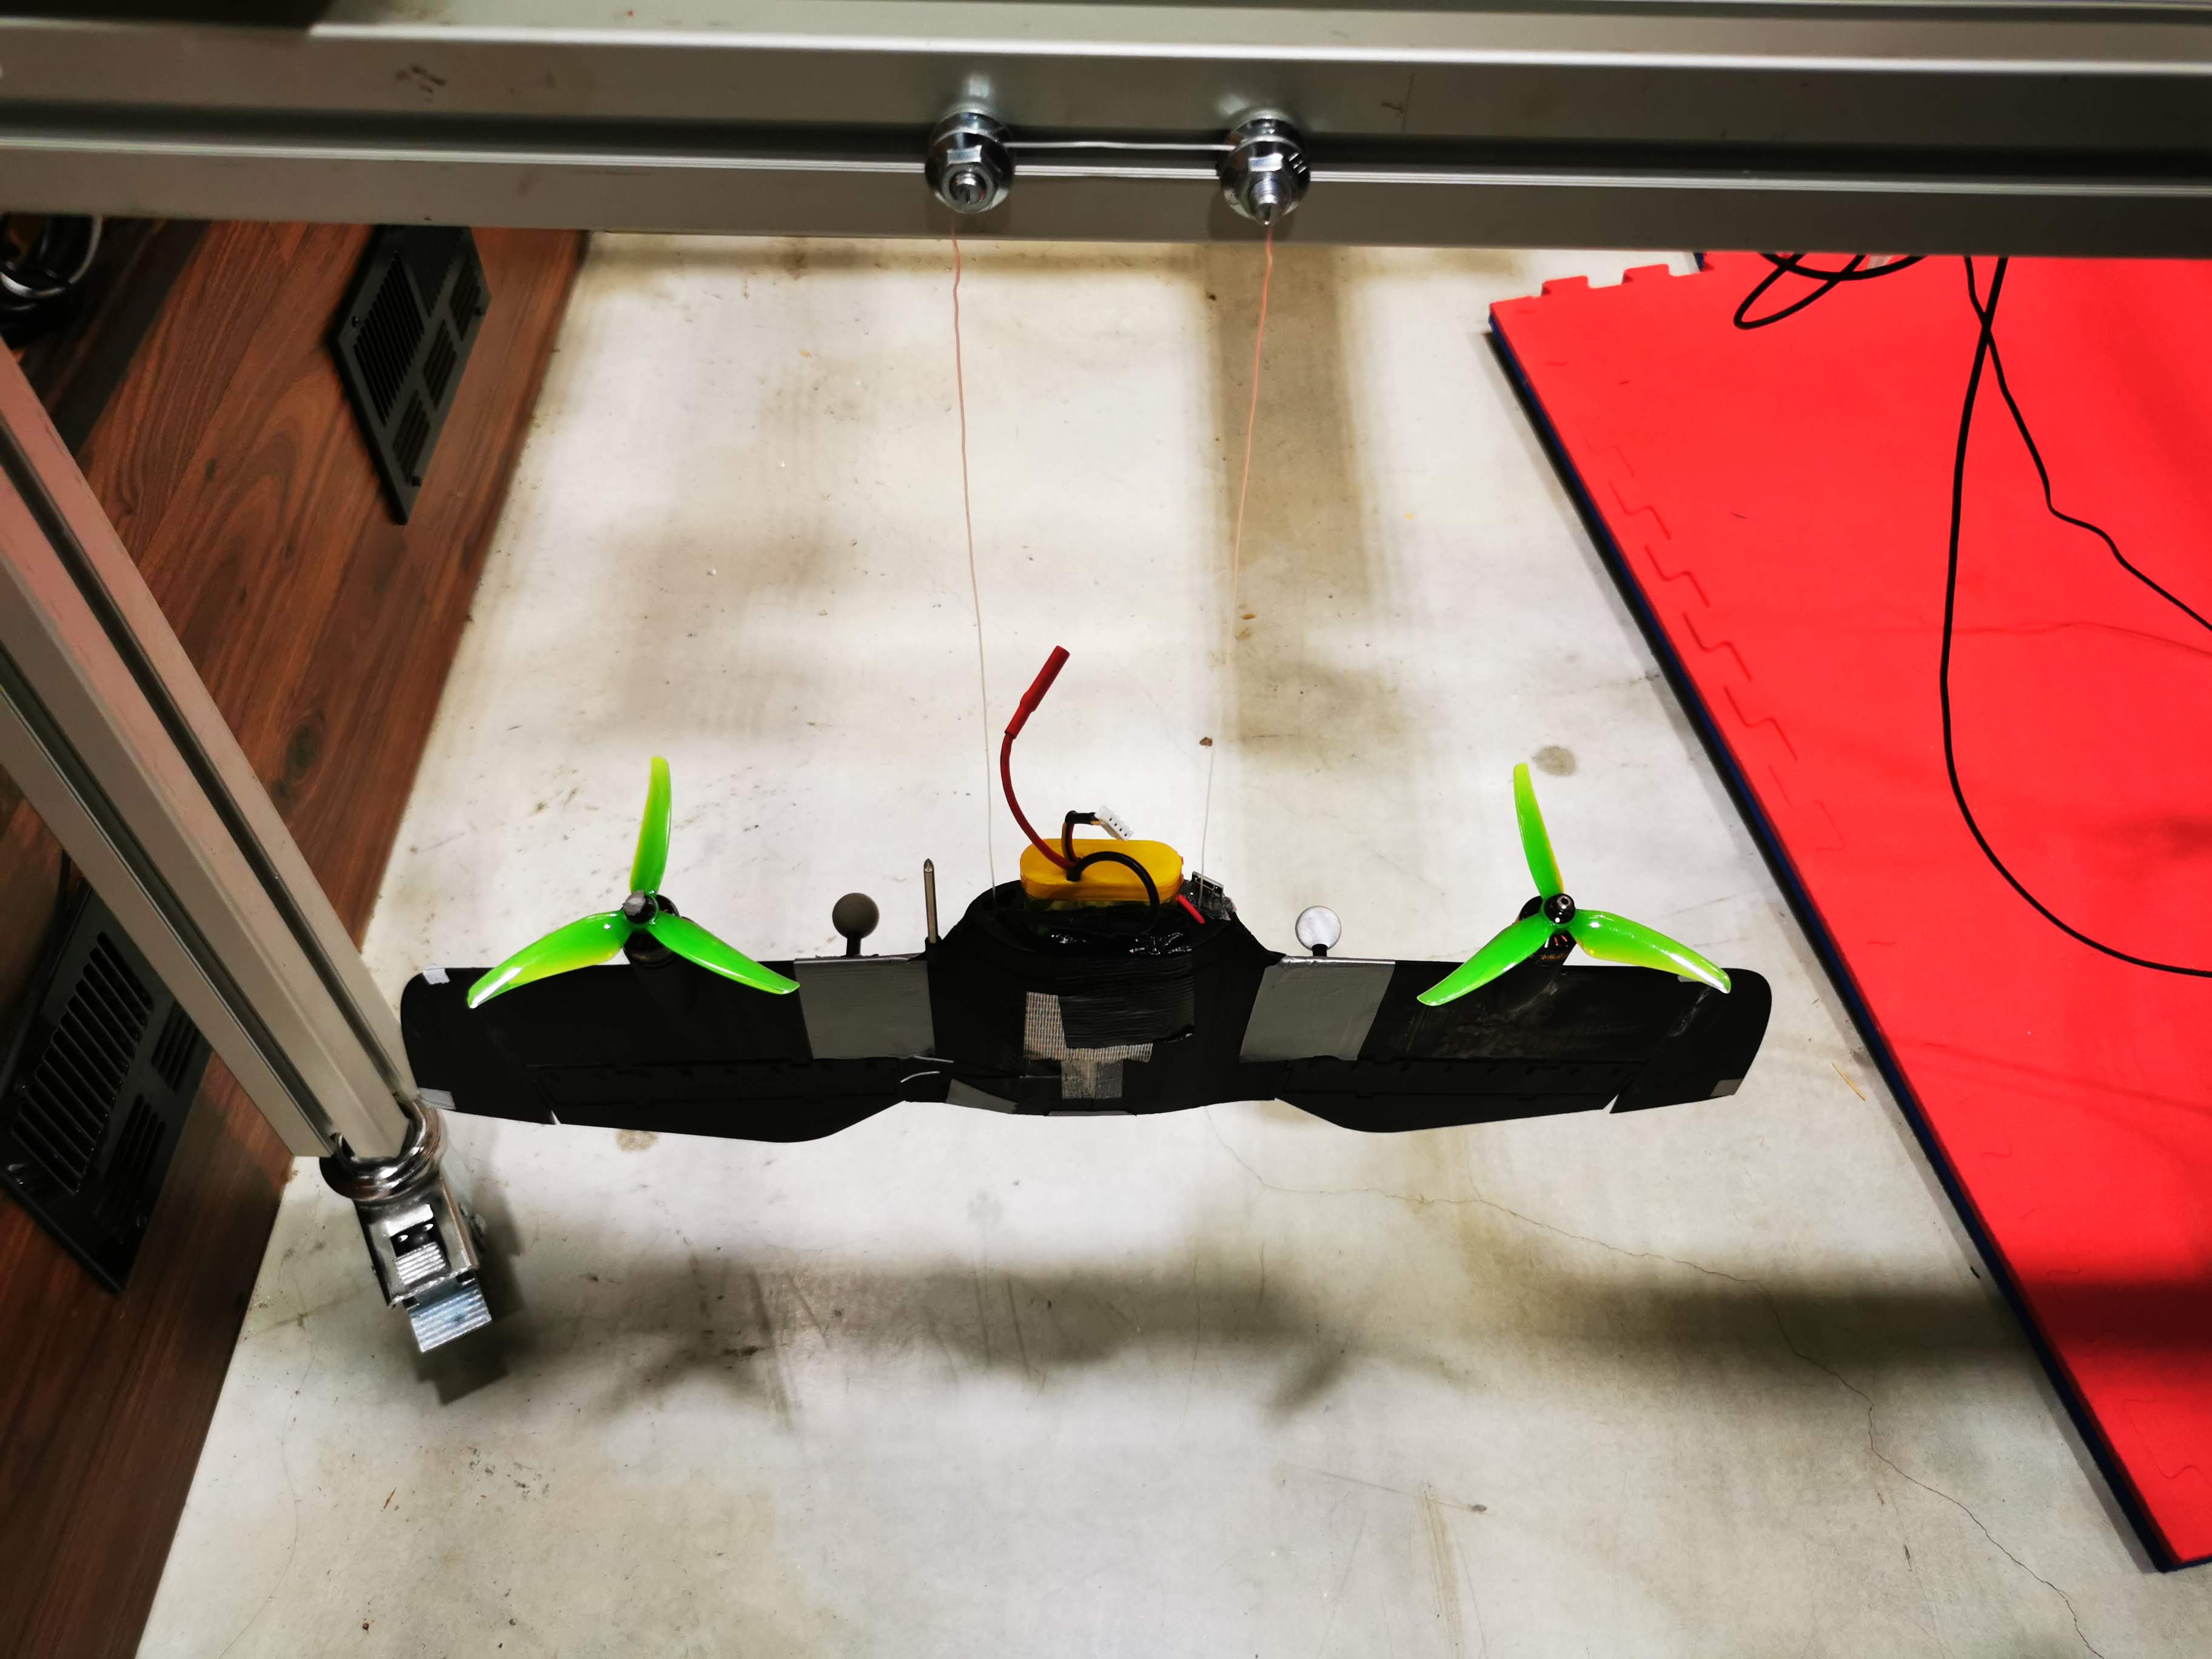
\includegraphics[trim=20cm 15cm 23cm 0cm,clip,width=0.4\columnwidth]{figures/IMG_20230609_085023.jpg}}
        \caption{Montage d'un pendule bifilaire pour l'identification de l'inertie ($\boldsymbol{J}$) de DarkO.}
        \label{fig:BifilarPend}
    \end{figure}

    Lors de la mesure, l'autopilote est utilisé pour réaliser une acquisition, à 500 Hz, de l'orientation du drone. Le drone est positionné avec un angle non nul vis-à-vis de la position d'équilibre du pendule bifilaire puis il est lâché sans vitesse initiale. Le couple de rappel engendré par les deux fils engendre des oscillations amorties (Voir la figure \ref{fig:BifilarPend_meas}). Il est nécessaire de connaitre la longueur des fils $h$ ainsi que leur écartement $D$ pour réaliser l'identification. Ces valeurs sont mesure directement sur le banc de mesure pour chacune des trois configurations.

    Une fois la mesure réalisée, nous utilisons l'outil \textit{Simulink Design Optimization} pour obtenir les valeurs de l'amortissement visqueux $C$, et de l'inertie sur l'axe mesuré $I$ à partir du modèle suivant :
    \begin{align*}
        \ddot{\theta} +  \frac{C}{I}\dot{\theta} + \left(\frac{mgD^2}{4Ih}\right)\frac{\sin\theta}{\sqrt{1 - 0.5\left(\frac{D}{h}\right)^2(1 - \cos\theta)}} = 0
    \end{align*}
    où $\theta$ est l'angle mesuré par l'autopilote à l'aide du code d'estimation d'état utilisant le gyroscope, l'accéléromètre et l'Optitrack.
    

    \begin{figure}[ht!]
    \centerline{
    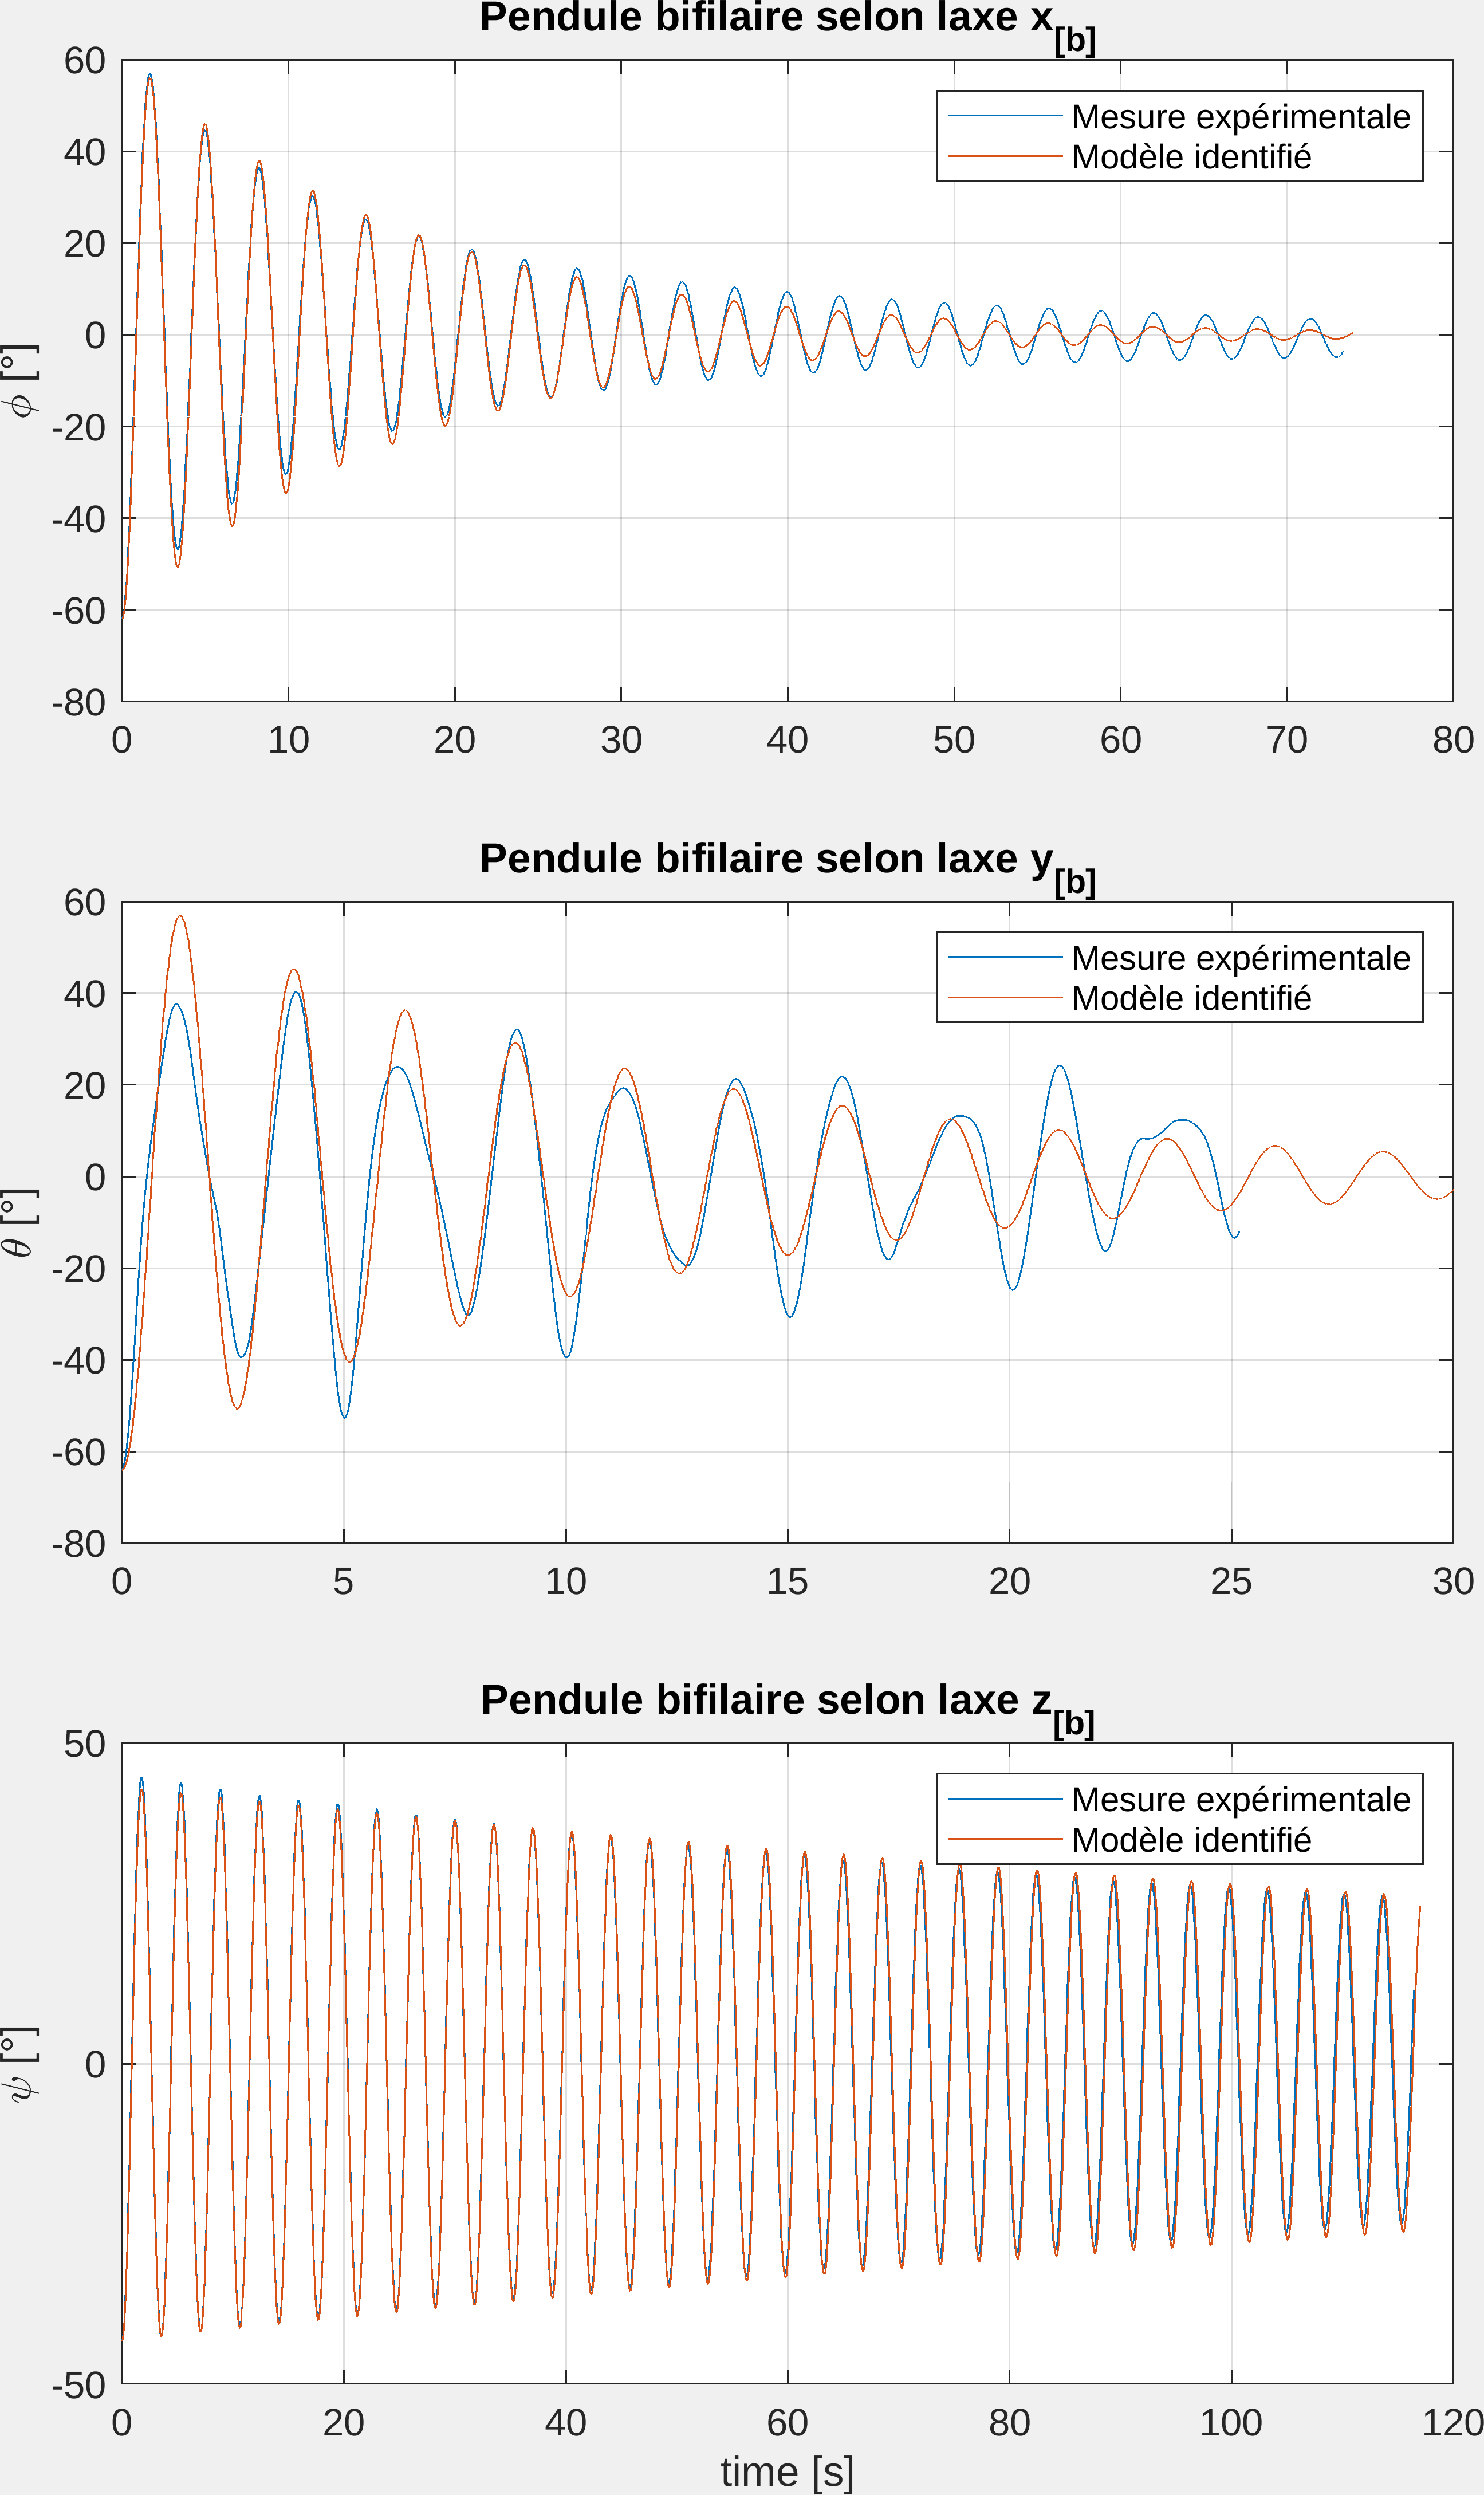
\includegraphics[trim=0cm 0cm 0cm 0cm,clip,width=0.6\columnwidth]{figures/ident_inertia.png}}
    \caption{Identification de l'inertie ($\boldsymbol{J}$), à partir des mesures issues du pendule bifilaire \ref{fig:BifilarPend}.}
    \label{fig:BifilarPend_meas}
    \end{figure}
    \todo{ajouter explication sur l'indentification}


    
    Les autres coefficients ont été estimés à l'aide d'un montage sur un capteur de force et moment à 6 DOF.
    \begin{figure}[ht!]
        \centering
        \resizebox{.9\textwidth}{!}{%
        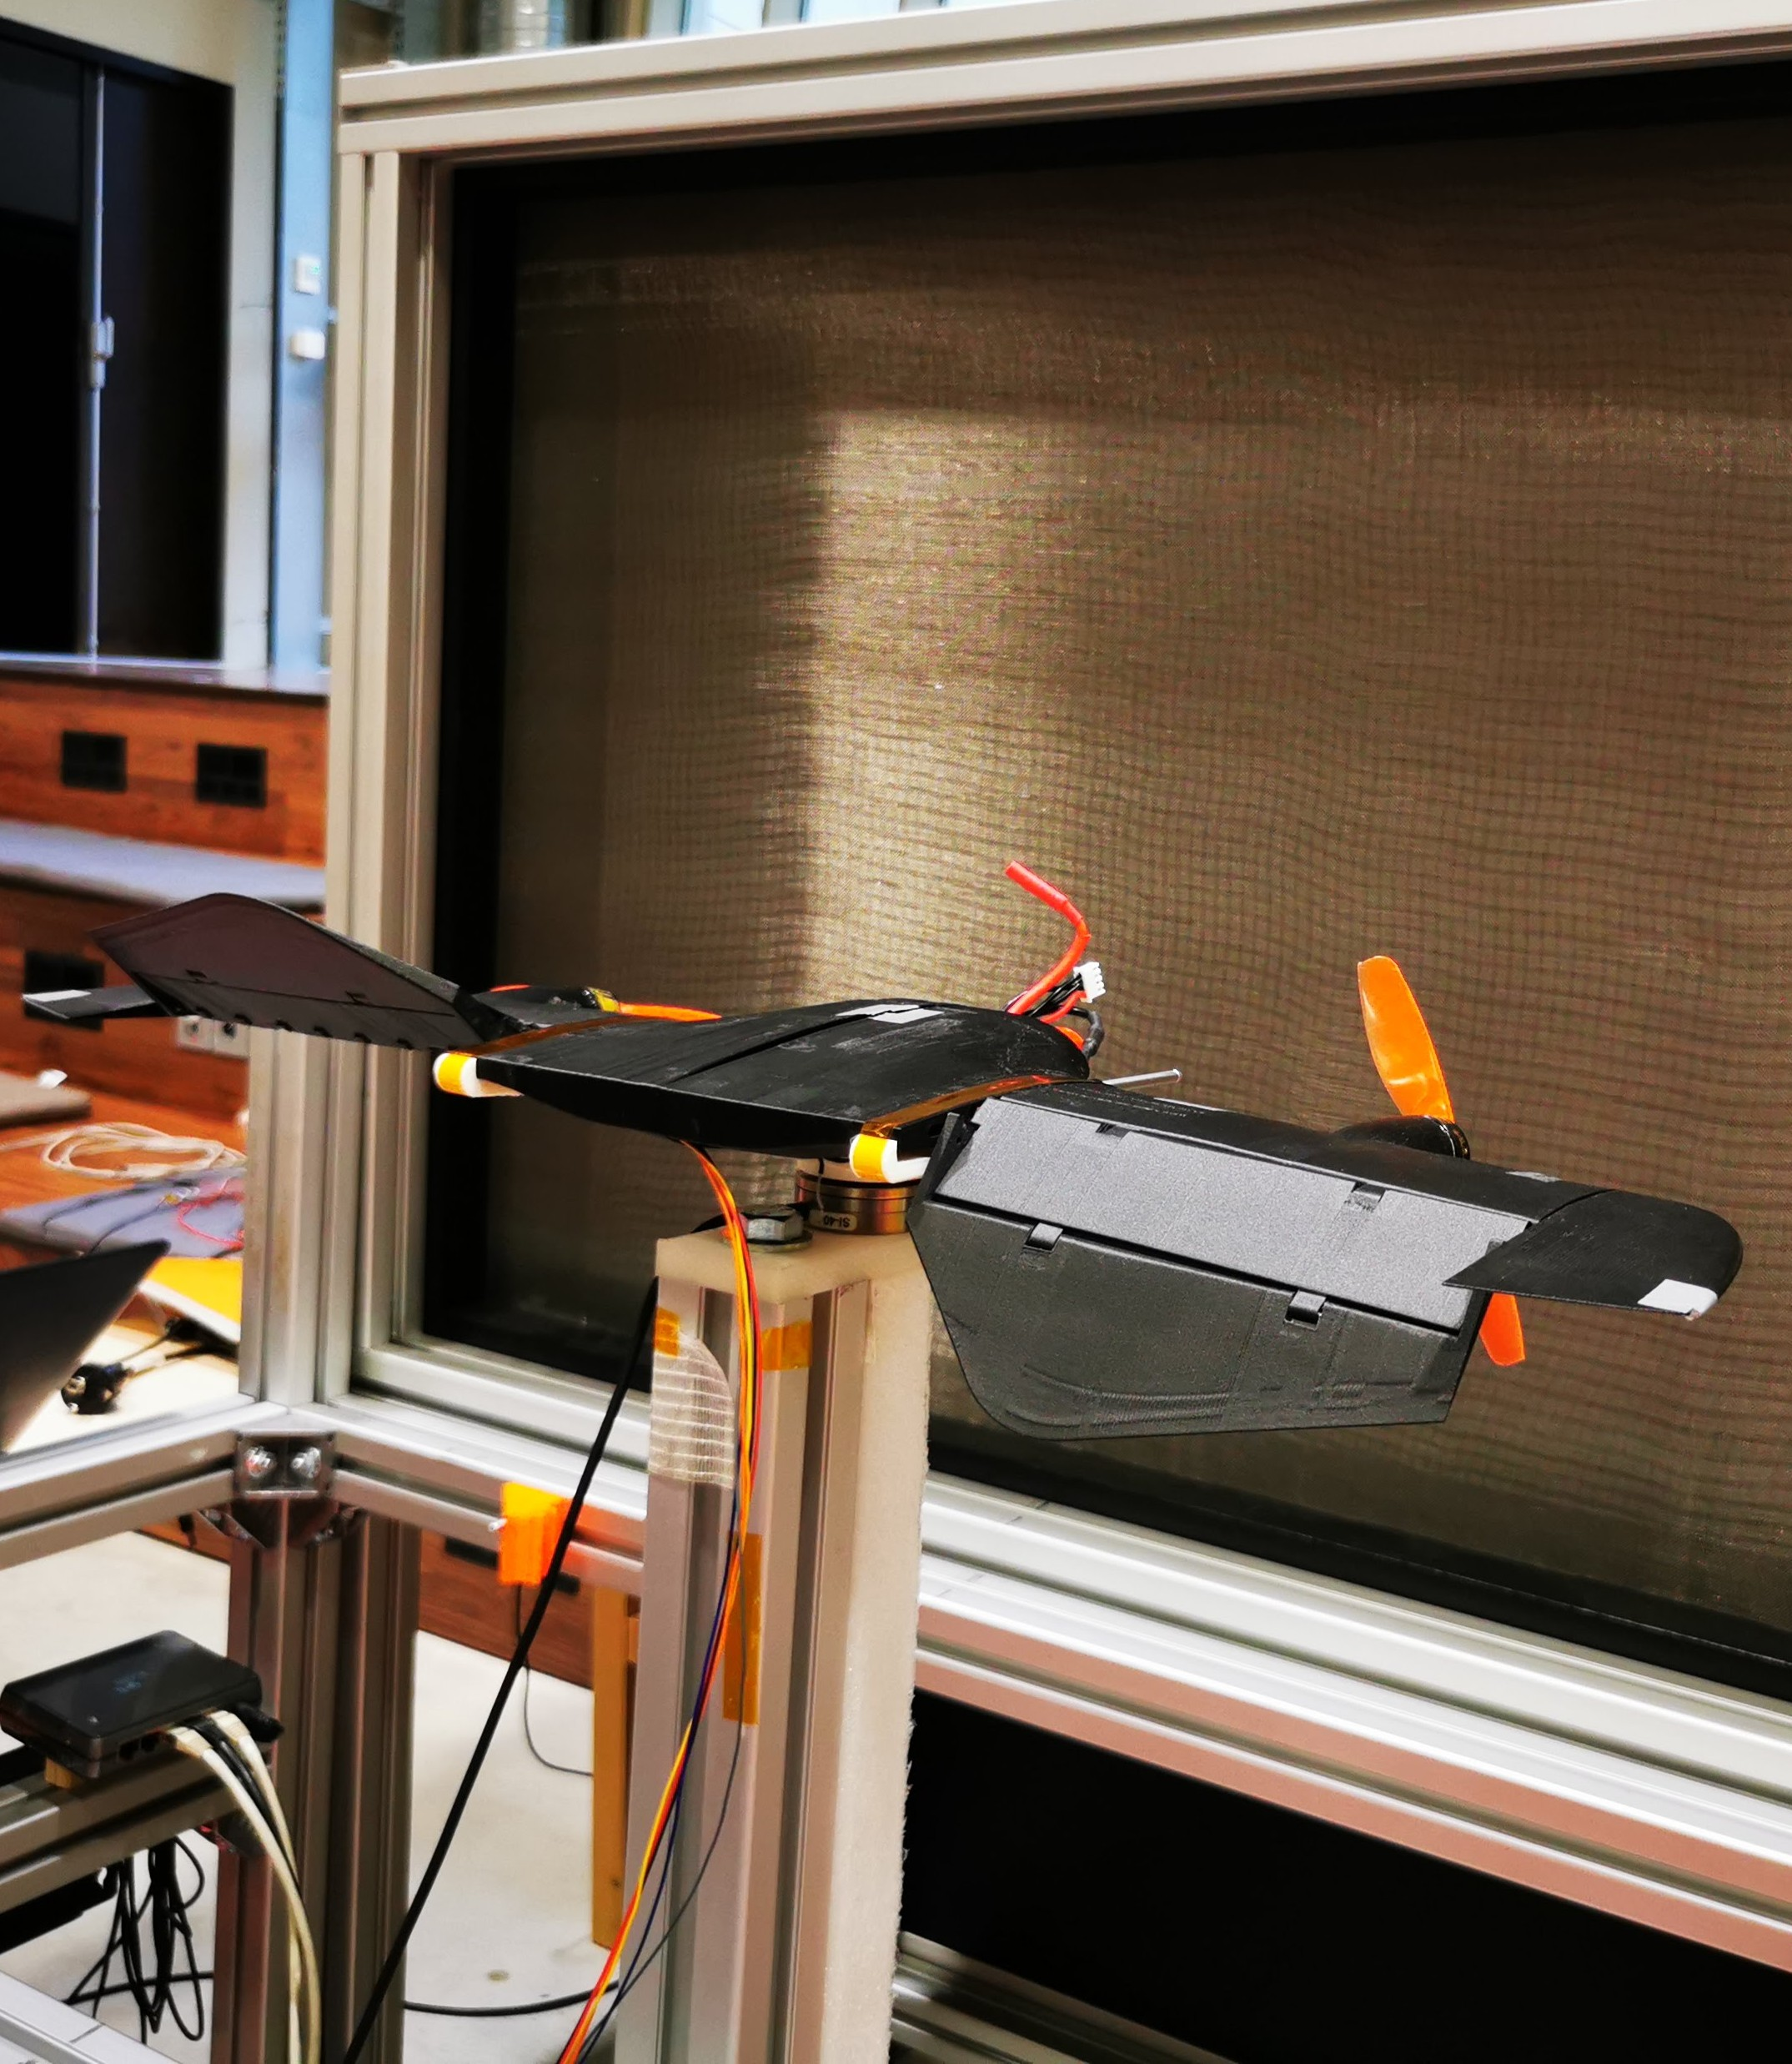
\includegraphics[height=3cm]{figures/montage_ident_arr.jpg}
        \quad
        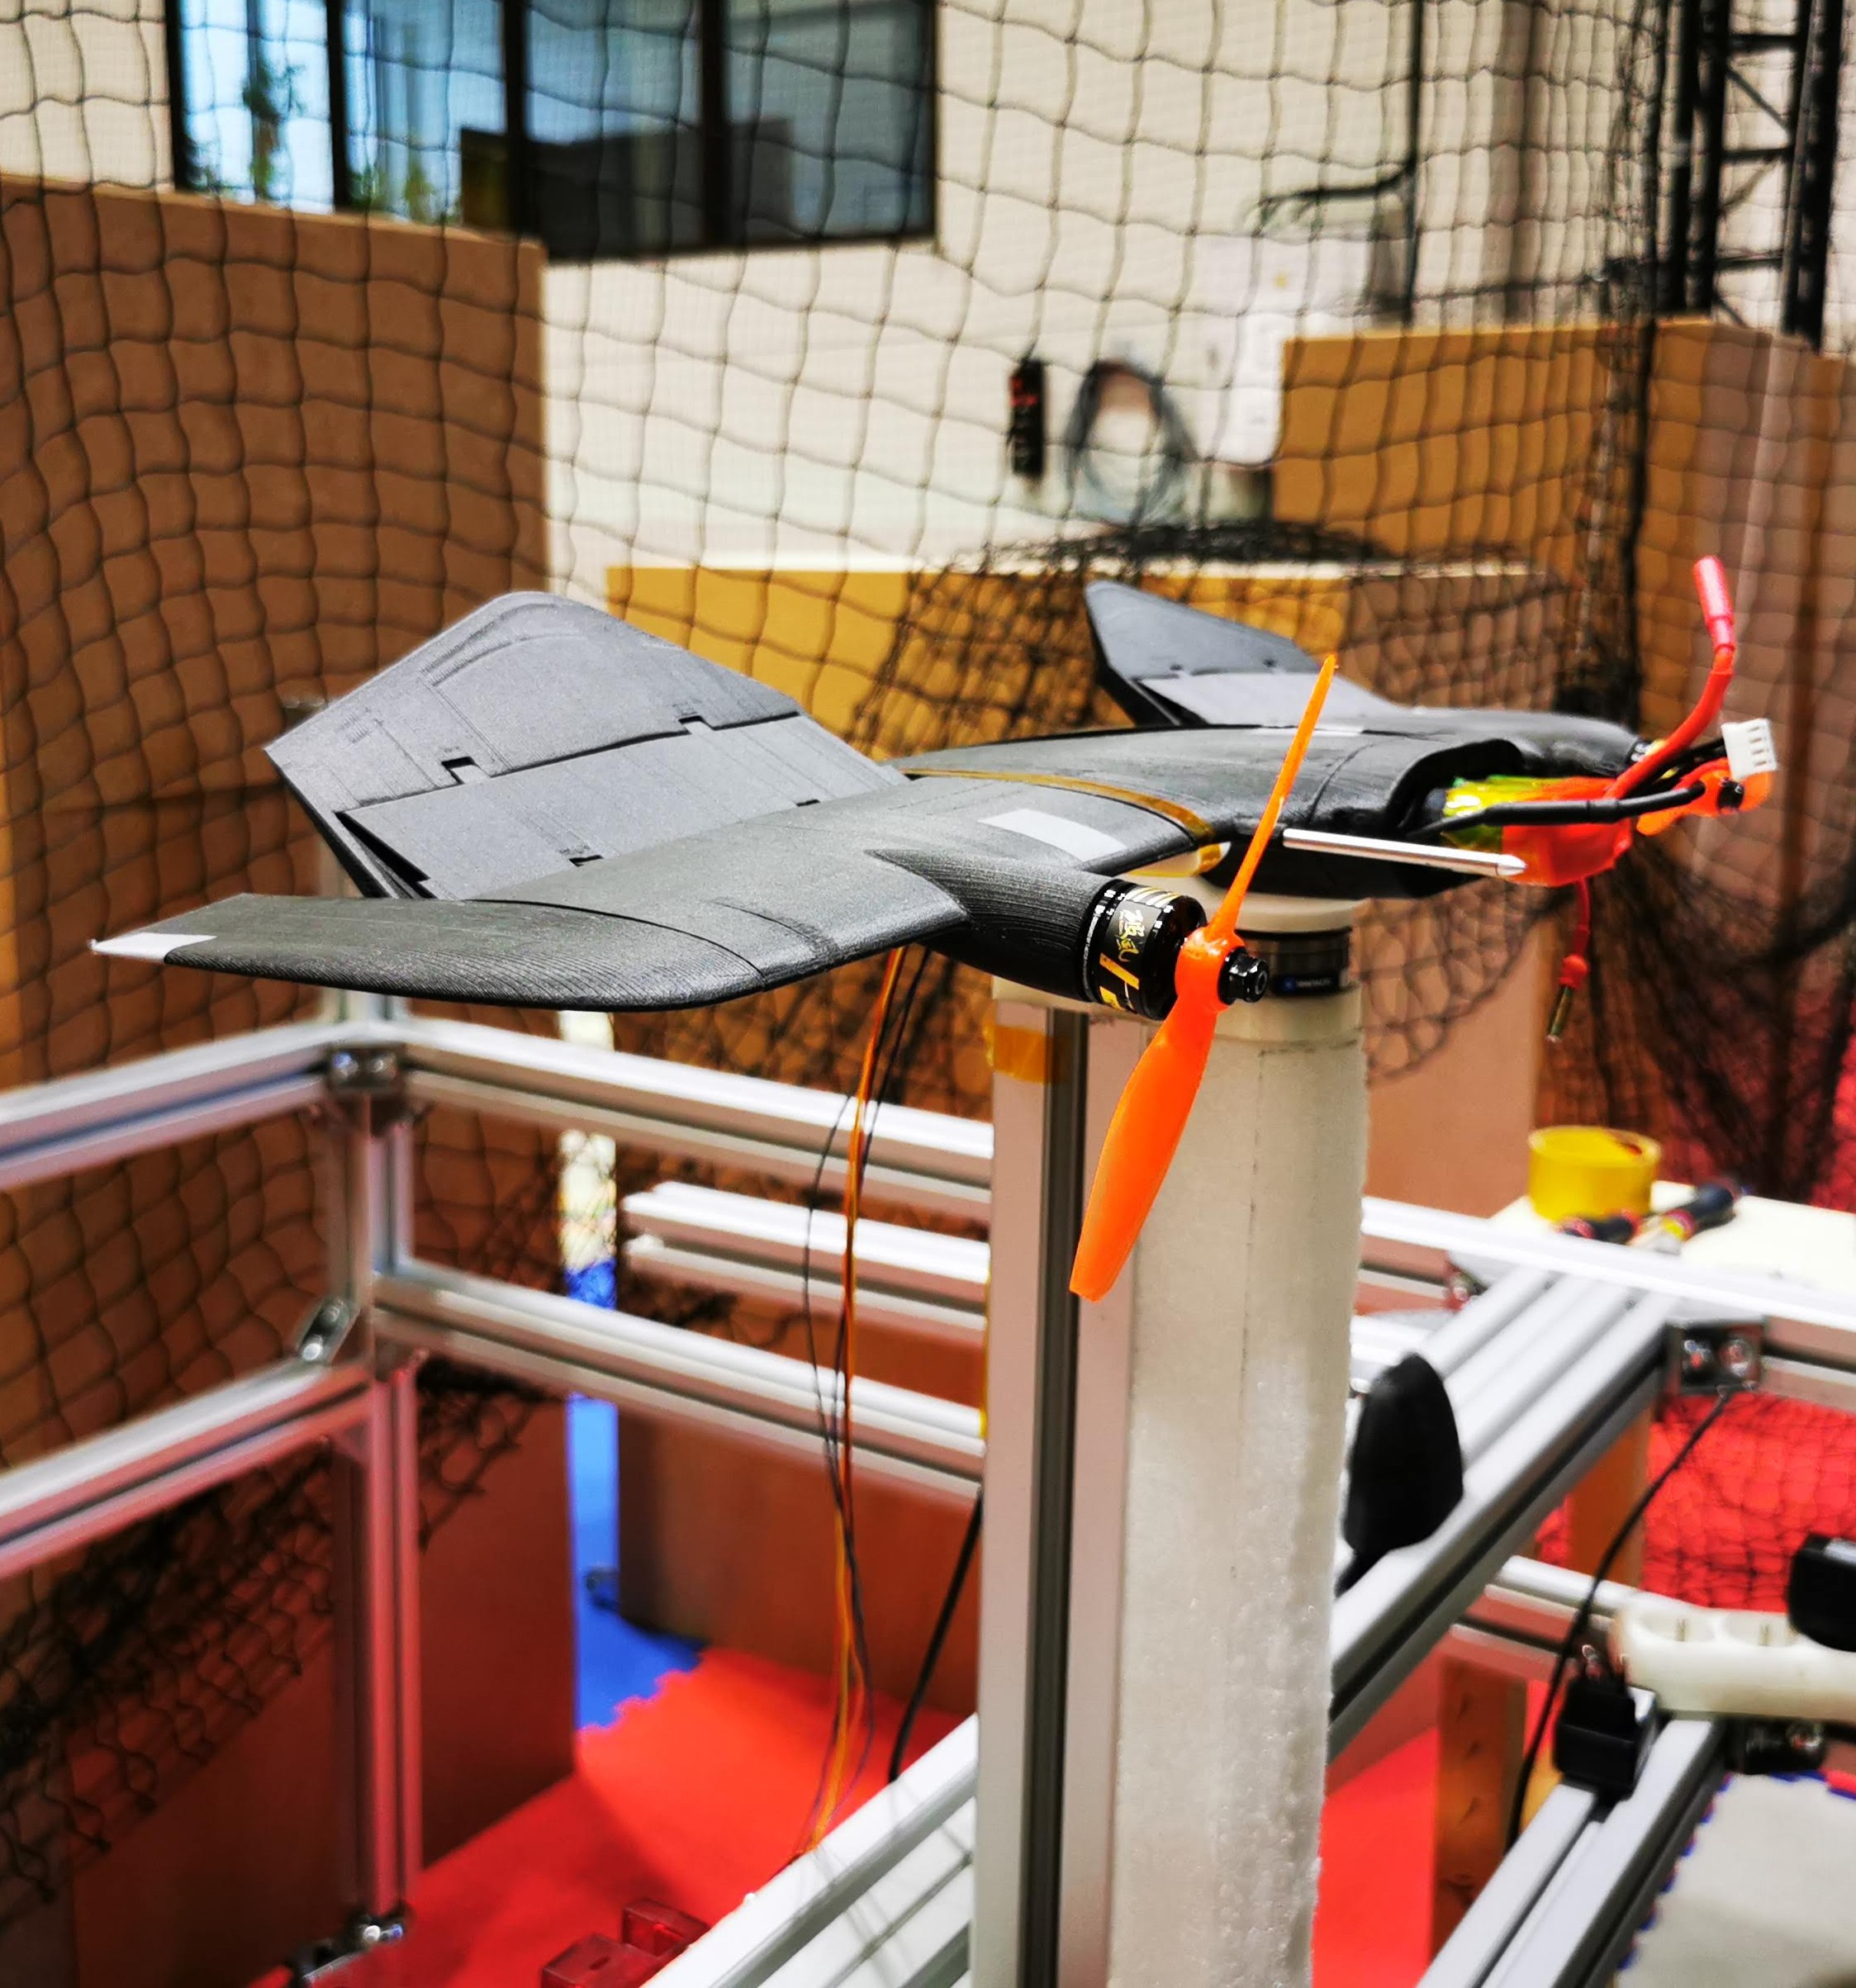
\includegraphics[height=3cm]{figures/montage_ident_face.jpg}
        }
        \caption{Montage de DarkO sur un banc de mesure face à une soufflerie ouverte.}
        \label{fig:montage_ident}
    \end{figure}
    Ces mesures permettent d'estimer la surface. Il est intéressant de noter que la surface soufflée par les hélices représente 67 \% de la surface totale du drone.
    

\subsection{Modélisation des actionneurs}
    \label{sec:saturation}
    Les actionneurs de DarkO ont des dynamiques qui limitent leur action en terme d'amplitude et de vitesse.

    Pour les moteurs électriques générant la traction par les hélices, il existe deux causes de saturation. Une saturation à haute vitesse liée à  la tension maximale du moteur et une saturation basse vitesse liée à la vitesse minimale de commutation de bobine du moteur, pour maintenir la rotation. De plus, ces saturations permettent d'obtenir un modèle réaliste à énergie finie. Elles correspondent à la contrainte suivante : $\omega_i \in [2500,~16000]~rpm = [262,~1675]~\SI{}{\radian\per\second}$, $i=1,2$. En termes de dynamique, nous avons représenté la chaîne d'actionnement du moteur (composée de l'ESC, du moteur et de l'hélice) par une fonction de transfert du premier ordre ayant une constante de temps égale à \SI{0,0125}{\second}, ce qui fournit un système d'actionnement assez agressif.

    Les saturations impactant les élevons proviennent des limites physiques des servomoteurs et du débattement limité par la forme de l'UAV, $\delta_i \in [-30~; 30]\text{\textdegree}$, $i=1,2$. La saturation la plus importante ici est peut-être la bande passante de l'actionneur (due à l'actionnement du servomoteur), qui est modélisée par une fonction de transfert du premier ordre avec une constante de temps \SI{0,05}{\second}. 

\section{Équilibres stationnaires}
    \subsection{Équilibre stationnaire sans vent}
        \label{sec:eq_nowind}

        Nous proposons une modification du vecteur de commande, dans le cas d'un équilibre sans vent $\boldsymbol{w}_{\mathrm{eq}} = 0$, basé sur le couplage des actionneurs. 
        \begin{align}
            \label{eq:vector_u_nowind}
            \boldsymbol{u}_{\text{nowind}} := \begin{bmatrix}\tau_{1}  \!&\! \tau_{2}  \!&\! \delta_{1}\tau_{1} \!&\! \delta_{2}\tau_{2} \end{bmatrix}^\top
        \end{align}
        Nous soulignons que le vecteur $\boldsymbol{u}_{\text{nowind}}$ dans \eqref{eq:vector_u_nowind} correspond à une transformation non inversible des actionneurs de DarkO correspondant à $\boldsymbol{u} := \begin{bmatrix}\tau_{1}  \!&\! \tau_{2}  \!&\! \delta_{1} \!&\! \delta_{2} \end{bmatrix}^\top$ (\eqref{eq:vector_u}). Néanmoins, si l'on impose les contraintes de saturation décrites dans la section~\ref{sec:saturation}, il est possible de déterminer de manière unique $\boldsymbol{u}$ à partir d'une valeur souhaitée de $\boldsymbol{u}_{\text{nowind}}$ dans \eqref{eq:vector_u_nowind}, car les valeurs positives non nulles de $\tau_{1}$ et $\tau_{2}$ peuvent être déterminées à partir des deux premières composantes de $\boldsymbol{u}_{\text{nowind}}$, puis $\delta_1$ et $\delta_2$ sont facilement construites à partir des deux dernières composantes de $\boldsymbol{u}_{\text{nowind}}$. 

        Nous obtenons un modèle linéaire vis-à-vis de sa commande, dérivé de \eqref{eq:dyna_simp} en imposant  $\boldsymbol{w} = 0$,
        \begin{subequations}\label{eq:withouwind}
        \begin{align}
                \boldsymbol{\dot p} &=  \boldsymbol{v}, \quad &
                m\boldsymbol{\dot v} &= - m\boldsymbol{g} +  \boldsymbol{R}(\boldsymbol{q})\boldsymbol{F}\boldsymbol{u}_{\text{nowind}},\\
                \boldsymbol{\dot q} &= \frac{1}{2}\boldsymbol{q} \otimes \smallmat{0 \\ \boldsymbol{\omega}_{\text{b}}} \quad & \boldsymbol{J} \boldsymbol{\dot \omega}_{\text{b}} &= \! \shortminus \skewsym{\boldsymbol{\omega}_{\text{b}}}\!J\boldsymbol{\omega}_{\text{b}} \! + \! \boldsymbol{M}\boldsymbol{u}_{\text{nowind}},
        \end{align}
        \end{subequations}
        avec les matrices
        \begin{align}
            \label{eq:FandM}
            \left[ \begin{array}{c|c}\!\boldsymbol{F}\!&\!\boldsymbol{M}\!\end{array} \right] := \left[ \begin{array}{cccc | cccc} a_{\text{f}} & a_{\text{f}} & 0 & 0 & a_{\text{m}} & -a_{\text{m}} & b_{\text{m}} & -b_{\text{m}} \\  0 & 0 & 0 & 0 & 0 & 0 & c_{\text{m}} & c_{\text{m}} \\ 0 & 0 & b_{\text{f}} & b_{\text{f}} & d_{\text{m}} & -d_{\text{m}} & 0 & 0 \end{array} \right]
        \end{align}
        et les scalaires
            \begin{align*}
                \left[\!\! \begin{array}{c|c} 
                a_{\text{f}} & b_{\text{f}} \\ \hline
                a_{\text{m}} & b_{\text{m}} \\ \hline
                c_{\text{m}} & d_{\text{m}}
                \end{array} \!\!\right] \!=\!
                \left[\begin{array}{c|c}
                1-\frac{S_{\text{wet}}}{4S_{\text{p}}} C_{\text{d}}  & -\frac{S_{\text{wet}}}{4S_{\text{p}}}C_{\ell}\xi_{\text{f}} \\ \hline
                \frac{k_{\text{m}} }{k_{\text{f}}}  &   \! \frac{S_{\text{wet}}}{4S_{\text{p}}}a_{y}C_{\ell}\xi_{\text{f}} \!\\ \hline
                \!\! \frac{S_{\text{wet}}}{4S_{\text{p}}} \Delta_{\text{r}}C_{\ell}\xi_{\text{m}} \!\! & 
                p_{y}+\frac{S_{\text{wet}}}{4S_{\text{p}}} a_{y} C_{\text{d}}
                \end{array}\right].
            \end{align*}


        Tous les couples d'équilibre $(\boldsymbol{u}_{\text{nowind}}, \boldsymbol{x}) = (\boldsymbol{u}_{\text{nowind},\text{eq}}, \boldsymbol{x_{\text{eq}}})$ sont paramétré par une rotation arbitraire autour de l'axe $z_{[\text{i}]}$ définit par $\beta \in \left[-\sqrt{\frac{1}{2}},\sqrt{\frac{1}{2}}\right]$. Le point d'équilibre a pour expression
        \begin{subequations}
            \label{eq:equilibria}
            \begin{align}
                \label{eq:bar_u}
                \boldsymbol{u}_{\text{nowind},\text{eq}} = \frac{mg}{( 1-\frac{S_{\text{wet}}}{4S_{\text{p}}} C_{\text{d}})} [1~1~0~0]^\top\\
                \boldsymbol{q}_{\text{eq}} = [\eta_{\text{eq}} ~\boldsymbol{\epsilon}_{\text{eq}}^\top]^\top = \smallmat{\sqrt{\frac{1}{2}-\beta} & \beta & \frac{2\beta^{2}-1}{2\sqrt{\frac{1}{2}-\beta}} & \beta}^\top.
            \end{align}
        \end{subequations}
        En présence d'un vent nul, le degré de liberté $\beta$ permet d'orienter le drone dans n'importe quelle direction horizontale.

    \subsection{Équilibre stationnaire en présence de vent}
    À partir des modèles \eqref{eq:dyna_orig} et \eqref{eq:dyna_simp}, nous caractérisons un équilibre stationnaire en présence d'un vent constant $\boldsymbol{w}_{\mathrm{eq}} =\smallmat{w_x \\ w_y \\w_z} \in \real^3$ exprimé dans le repère inertiel, tel que $\smallmat{w_x \\ w_y} \neq 0$, c'est-à-dire qu'il existe toujours un vent horizontal non nul.
    Ainsi, pour chaque position de référence $\boldsymbol{p}_{\text{eq}} \in \real^3$, 
    un ensemble de couple état/commande possible est $(\boldsymbol{u}_{\text{eq}}, \boldsymbol{x}_{\text{eq}}) = (\boldsymbol{u}_{\text{eq}}, \boldsymbol{p}_{\text{eq}}, \boldsymbol{v}_{\text{eq}}, \boldsymbol{q}_{\text{eq}}, \boldsymbol{\omega}_{\text{b},\text{eq}})$
    obtenu à l'aide de
    \begin{subequations}
    \label{eq:equilibrium}
    \begin{align}
    \label{eq:ueq}
            &\boldsymbol{u}_{\text{eq}} = \begin{bmatrix} \tau & \tau & \delta & \delta \end{bmatrix}^\top\\
            & \boldsymbol{q}_{\text{eq}} = \boldsymbol{q}_{\mathrm{eq}\psi} \otimes  \boldsymbol{q}_{\mathrm{eq}\theta} \label{eq:qeq}\\
            &\boldsymbol{\omega}_{\text{b},\text{eq}} = 0 , \quad \boldsymbol{v}_{\text{eq}} = 0, 
    \end{align}
    \end{subequations}
    où nous définissons deux quaternions $\boldsymbol{q}_{\mathrm{eq}\psi}$ et $\boldsymbol{q}_{\mathrm{eq}\psi}$ permettant d'exprimer l'ensemble des conditions de vent dans le repère inertiel vers un repère tourné où le vent est toujours contenu dans le plan $x-z$. Grâce à cette transformation, nous exprimons un ensemble continue d'équilibre en présence de vent. 

    \begin{align}
    \label{eq:qtheta}
        \boldsymbol{q}_{\mathrm{eq}\theta} &:= \begin{bmatrix} \cos(\frac{\theta}{2}) & 0 & \sin(\frac{\theta}{2}) & 0 \end{bmatrix}^\top
    \end{align}
    \begin{align}
    \label{eq:qpsi}
        \boldsymbol{q}_{\mathrm{eq}\psi} &:= \begin{bmatrix} \cos(\frac{\psi}{2}) & 0 & 0 & \sin(\frac{\psi}{2}) \end{bmatrix}^\top.
    \end{align}
    Les paramètres de l'équilibre sont la rotation horizontale $\psi = \arctan(w_{x}, w_{y})$, l'angle d'inclinaison $\theta$, la poussée des hélices $\tau$, et la déflexion des élevons $\delta$. Ils peuvent être obtenus à partir de l'algorithme~\ref{alg:eq}. 

    \begin{algorithm}
    \caption{Obtention des paramètres d'équilibre en \eqref{eq:equilibrium}.}
    \label{alg:eq}
    \hspace*{.1cm} \textbf{Entrée} : Vecteur vent $\boldsymbol{w}_{\text{eq}} =\smallmat{w_x & w_y & w_z}^\top$ \\
    \hspace*{.1cm} \textbf{Sortie} : Paramètres $\psi$, $\theta$, $\tau$, $\delta$ dans \eqref{eq:equilibrium}
    \begin{algorithmic}[1]
        %\Require {\bf Input} values: $\boldsymbol{w} =\smallmat{w_x & w_y & w_z}^\top$ 
        %\Ensure  $\psi$, $\theta$, $\tau$, $\delta$
        \State Détermine l'angle $\psi = \text{atan2}(w_x, w_y)$ de manière à obtenir $\boldsymbol{q}_{\mathrm{eq}\psi}$ dans \eqref{eq:qpsi}  
        \State Détermine la perturbation tournée $\boldsymbol{w}_{\text{r}}$ avec la composante $y$ nulle, en utilisant $\boldsymbol{R}_{\psi}:= \smallmat{ \cos \psi & \sin \psi & 0 \\ -\sin \psi & \cos \psi & 0 \\ 0 & 0 & 1 }$, selon
        \begin{align}
        \label{eq:wh}
        \boldsymbol{w}_{\mathrm{r,eq}} := \smallmat{w_{\text{r}x} \\ 0 \\w_{\text{r}z}} :=  \boldsymbol{R}^\top(\boldsymbol{q}_{\mathrm{eq}\psi}) \boldsymbol{w}_{\mathrm{eq}} = \boldsymbol{R}^\top_{\psi} \boldsymbol{w}_{\mathrm{eq}}
        \end{align}

        \State Détermine l'angle d'inclinaison $\theta$ de manière à obtenir $\boldsymbol{q}_{\text{eq}\theta}$ dans \eqref{eq:qeq}:  
        \begin{align}
        \label{eq:theta_alg}
            \theta = -\tan^{-1}\left(\frac{w_{\text{r}z}}{w_{\text{r}x}} + \frac{2mg}{\rho S \lVert \boldsymbol{w}_{\mathrm{eq}} \rVert C_{\ell}  (1-\frac{\xi_{\text{f}}}{\xi_{\text{m}}}) w_{\text{r}x} } \right)
        \end{align}
    \State Pour des raisons de commodité, nous définissons les scalaires 
        $$ 
        \left[\begin{array}{c|c} 
        \!\!a\!\!&\!\!b\!\! \\ \hline \!\!c\!\!&\!\! d\!\!\end{array}  \right] \!:=\! 
        \left[\begin{array}{c|c}
        2 S_{\text{wet}} C_{\ell} mg \sin{\theta} \xi_{\text{f}} &
        \! 2 S_{\text{wet}} C_{\text{d}} C_{\ell} \rho  \lVert \boldsymbol{w}_{\mathrm{eq}} \rVert  w_{x}^{\text{b}}\!\! \\ \hline
        \!\!-4 S S_{\text{p}} C_{\ell} \rho  \lVert \boldsymbol{w}_{\mathrm{eq}} \rVert  w_{x}^{\text{b}} \xi_{\text{f}}\!\! & \frac{b \xi_{\text{f}}}{2}
        \end{array}\right]
        $$ 
        et grâce à ces scalaires $(a,b,c,d)$, déterminons la traction des hélices $\tau$ dans \eqref{eq:ueq} comme
        \begin{align}
            \nonumber
            \tau &= \frac{S_{\text{p}}}{2 S_{\text{wet}} C_{\ell} \xi_{\text{f}} (4S_{\text{p}} -  S_{\text{wet}} C_{\text{d}} )} \Bigg( a+b+c+d + \Bigg[ (a+b+c \shortminus d)^2 \shortminus 4 (d^2+ac \shortminus bd)  \\ 
            & \quad
            \shortminus \frac{4 {w_{z}^{\text{b}}}^2 d}{ {w_{x}^{\text{b}}}^2 } (d+c) + \frac{4 w_{z}^{\text{b}}ad\cos{\theta}}{w_{x}^{\text{b}} C_{\ell} \sin{\theta} } \left(C_{\text{d}} - \frac{4 S_{\text{p}}}{S_{\text{wet}}}\right) \Bigg] ^{\frac{1}{2}} \Bigg),\label{eq:tau_alg}
        \end{align}
        où
        $$
        \bigmat{w_{x}^{\text{b}} \\ w_{z}^{\text{b}}} = \bigmat{   w_{\text{r}x} \cos{\theta} - w_{\text{r}z} \sin{\theta}\\
                    w_{\text{r}x} \sin{\theta} +  w_{\text{r}z} \cos{\theta} }.
        $$
        
        \State Déterminons la déflexion des élevons $\delta$ comme
        \begin{align}
        \label{eq:delta_alg}
            \delta = \frac{2mg\sin{\theta}}{\rho S \lVert \boldsymbol{w}_{\mathrm{eq}} \rVert C_{\text{d}}\xi_{\text{f}} w_{z}^{\text{b}}} + \frac{w_{x}^{\text{b}}}{\xi_{\text{f}}w_{z}^{\text{b}}} -  \frac{(4-\frac{S_{\text{wet}}}{S_{\text{p}}} C_{\text{d}})}{\rho S \lVert \boldsymbol{w}_{\mathrm{eq}} \rVert C_{\text{d}}\xi_{\text{f}} w_{z}^{\text{b}}} \tau.
        \end{align}

    \end{algorithmic}
    \hspace*{.1cm} \textbf{Retourne}:  $\psi$, $\theta$, $\tau$, $\delta$
    \end{algorithm}


    \begin{theorem}\label{thm:eqs}
    Pour tout vent constant, $\boldsymbol{w} =\smallmat{w_x & w_y & w_z}^\top \in \real^3$ ayant une composante horizontale non nulle $\smallmat{w_x \\ w_y}$,
    les équations \eqref{eq:qpsi}--\eqref{eq:qtheta} avec $\theta$, $\tau$ et $\delta$ sélectionné selon l'Algorithme~\ref{alg:eq} caractérisent un couple d'équilibre $(\boldsymbol{u}_{\text{eq}}, \boldsymbol{x}_{\text{eq}})$ pour la dynamique non linéaire \eqref{eq:dyna_orig} et \eqref{eq:dyna_simp}.
    
    \end{theorem}
    
    \begin{proof}
        Dans un premier temps, notons qu'avec l'expression de $\boldsymbol{R}$ \eqref{eq:matrix_rot} et l'expression de  $\psi$ dans l'étape 1 de l'Algorithme~\ref{alg:eq}, on peut définir la perturbation à l'équilibre tournée $\boldsymbol{w}_{\mathrm{r,eq}} := \boldsymbol{R}^\top_{\psi} \boldsymbol{w}_{\mathrm{eq}} :=    \boldsymbol{R}^\top(\boldsymbol{q}_{\mathrm{eq}\psi})\boldsymbol{w}_{\mathrm{eq}}$ (voir \eqref{eq:wh} dans l'Algorithme~\ref{alg:eq}),
        qui correspond à la rotation nécessaire pour aligner l'axe  $x_{[\text{b}]}$ du repère corps avec la direction du vent. Une fois que le drone est face au vent, il subit un vent avec une composante latérale $y$ nulle et il peut ajuster son angle d'inclinaison $\theta$ afin de générer la poussée et la portance nécessaires pour compenser les effets du vent dans les directions longitudinale et verticale (l'effet latéral est nul en raison de l'orientation spécifique de l'appareil $\psi$). Avec cette rotation $\psi$, il est possible d'exprimer le vent dans le repère corps comme étant
            \begin{align}
            \label{eq:wb}
                \boldsymbol{w}^{\text{b}}_{\mathrm{eq}} &:= 
                \begin{bmatrix}
                    w_{x}^{\text{b}} \\ 0 \\ w_{z}^{\text{b}}
                \end{bmatrix} \!=\! 
                \boldsymbol{R}^\top(\boldsymbol{q}_{\text{eq}\theta}) \boldsymbol{w}_{\mathrm{r,eq}}  \\
                &=\!\! \begin{bmatrix}
                    \cos{\theta} & 0 & -\sin{\theta}\\
                        0 & 1 & 0\\
                    \sin{\theta} & 0 & \cos{\theta}
                \end{bmatrix}^\top \!\! \begin{bmatrix}
                    w_{\text{r}x}\\
                    0\\
                    w_{\text{r}z}
                \end{bmatrix}
                \!\!=\!\!\begin{bmatrix}
                    w_{\text{r}x} \cos{\theta} - w_{\text{r}z} \sin{\theta}\\
                    0\\
                    w_{\text{r}x} \sin{\theta} +  w_{\text{r}z} \cos{\theta}
                \end{bmatrix}
            \nonumber
            \end{align}

        Nous insistons sur le fait que $w_{x}^{\text{b}}$ est toujours négatif et différent de zéro, car le drone est orienté dans la direction du vent grâce à la rotation engendré par $ \boldsymbol{q}_{\mathrm{eq}\psi}$, et suite à l'hypothèse $\smallmat{w_x \\ w_y} \neq 0$.
    
        L'équation \eqref{eq:dyna1} montre qu'il est nécessaire d'avoir $\boldsymbol{v}_{\text{eq}} = 0$ pour maintenir l'équilibre stationnaire. En multipliant \eqref{eq:dyna2} par $\boldsymbol{R}(\boldsymbol{q}_{\text{eq}})$ donné dans  \eqref{eq:wb}, nous l'exprimons dans le repère corps.
        Comme nous appliquons la même commande $\tau_{1} = \tau_{2} = \tau $ aux deux moteurs et la même commande au deux élevons $\delta_{1} = \delta_{2} = \delta$, nous obtenons pour les deux modèles \eqref{eq:dyna_orig} et \eqref{eq:dyna_simp}, l'équilibre des forces selon l'axe $x_{[\text{b}]}$ donné par
        \begin{align}
            & (2-\frac{S_{\text{wet}}}{2S_{\text{p}}} C_{\text{d}})\tau - \frac{1}{2}\rho S \lVert \boldsymbol{w}_{\mathrm{eq}} \rVert C_{\text{d}} \left(w_{x}^{\text{b}} - \xi_{\text{f}} \delta w_{z}^{\text{b}} \right) - mg \sin(\theta) = 0 \label{eq:forcex}
        \end{align}
        et l'équilibre des forces selon l'axe $z_{[\text{b}]}$ donné par
        \begin{align}\label{eq:forcez}
            - \frac{S_{\text{wet}}}{2S_{\text{p}}}\xi_{\text{f}} C_{\ell} \tau \delta - \frac{1}{2}\rho S \lVert \boldsymbol{w}_{\mathrm{eq}} \rVert C_{\ell} \left(w_{z}^{\text{b}} + \xi_{\text{f}} \delta w_{x}^{\text{b}} \right) + mg \cos(\theta) = 0
        \end{align}
        De manière similaire, à partir de \eqref{eq:dyna_orig_d} et \eqref{eq:dyna4}, l'équilibre des moments autour de l'axe $y_{[\text{b}]}$ permet d'obtenir
        \begin{align}\label{eq:momenty}
            \frac{S_{\text{wet}}}{2S_{\text{p}}}  \Delta_{\text{r}} \xi_{\text{m}} C_{\ell} \tau \delta + \frac{1}{2}\rho S \Delta_{\text{r}} \lVert \boldsymbol{w}_{\mathrm{eq}} \rVert C_{\ell} \left(w_{z}^{\text{b}} + \xi_{\text{m}} \delta w_{x}^{\text{b}} \right) = 0.
        \end{align}
        
        Pour calculer la solution du triplet ($\theta$,$\tau$,$\delta$) des trois équations d'équilibre \eqref{eq:forcex}--\eqref{eq:momenty}, ajoutons \eqref{eq:forcez} multiplié par $\Delta_{\text{r}} \xi_{\text{m}}$, à \eqref{eq:momenty} multiplié par $\xi_{\text{f}}$, de manière à annuler le premier terme et à obtenir
        \begin{multline*}
            \Delta_{\text{r}} \xi_{\text{m}} \left( - \frac{1}{2}\rho S \lVert \boldsymbol{w}_{\mathrm{eq}} \rVert C_{\ell} (w_{z}^{\text{b}} + \xi_{\text{f}} \delta w_{x}^{\text{b}}) + mg \cos(\theta) \right) \\+ \xi_{\text{f}} \left(\frac{1}{2}\rho S  \Delta_{\text{r}} \lVert \boldsymbol{w}_{\mathrm{eq}} \rVert C_{\ell} (w_{z}^{\text{b}} + \xi_{\text{m}} \delta w_{x}^{\text{b}})  \right) = 0,
        \end{multline*}
        qui est équivalent à
        \begin{align*}
            \frac{1}{2}\rho S  \Delta_{\text{r}} \lVert \boldsymbol{w}_{\mathrm{eq}} \rVert C_{\ell}  (\xi_{\text{f}} - \xi_{\text{m}}) w_{z}^{\text{b}} +   \Delta_{\text{r}} \xi_{\text{m}} mg \cos(\theta)  = 0,
        \end{align*}
        où ($w_{x}^{\text{b}}$,$w_{z}^{\text{b}}$) sont les première et troisième composantes de $\boldsymbol{w}^{\text{b}}$ dans \eqref{eq:wb}. Ensuite, en utilisant \eqref{eq:wb} et en réarrangeant, nous obtenons
        \begin{multline*}
                -\frac{1}{2}\rho S  \Delta_{\text{r}} \lVert \boldsymbol{w}_{\mathrm{eq}} \rVert C_{\ell}  (\xi_{\text{f}} - \xi_{\text{m}}) w_{\text{r}x} \sin{\theta}  +\bigg( -\frac{1}{2}\rho S  \Delta_{\text{r}} \\ \lVert \boldsymbol{w}_{\mathrm{eq}} \rVert C_{\ell}  (\xi_{\text{f}} - \xi_{\text{m}})w_{\text{r}z} +   \Delta_{\text{r}} \xi_{\text{m}} mg \bigg) \cos{\theta} = 0,
        \end{multline*}
        qui est satisfaite par
            \begin{align} \label{eq:theta}
                \theta &=  -\tan^{-1}\left(\frac{\rho S \lVert \boldsymbol{w}_{\mathrm{eq}} \rVert C_{\ell}  (\xi_{\text{f}} - \xi_{\text{m}})w_{\text{r}z} - 2 \xi_{\text{m}} mg }{\rho S\lVert \boldsymbol{w}_{\mathrm{eq}} \rVert C_{\ell}  (\xi_{\text{f}} - \xi_{\text{m}}) w_{\text{r}x}}\right).
            \end{align}
            Cette dernière expression coïncide avec la sélection \eqref{eq:theta_alg} dans l'Algorithme~\ref{alg:eq} après quelques manipulations.
        À partir de \eqref{eq:theta_alg}, nous pouvons calculer les commandes à l'équilibre en substituant \eqref{eq:forcex} dans \eqref{eq:forcez}. Après quelques simplifications, la force nécessaire de traction des hélices  $\tau$ pour maintenir la position d'équilibre corresponds à l'expression  \eqref{eq:tau_alg}. Finalement, avec la valeur de $\tau$ dans \eqref{eq:tau_alg}, nous pouvons obtenir la déflexion des élevons nécessaire $\delta$ à partir de l'équation \eqref{eq:forcez}, ce qui nous donne la valeur obtenue dans \eqref{eq:delta_alg}.
    \end{proof}
    Il est intéressant de noter que pour chaque couple de vent($w_{\text{r}z}$, $w_{\text{r}x}$) correspond une orientation d'équilibre \eqref{eq:qeq}, \eqref{eq:theta_alg} est indépendante de l'entrée $\boldsymbol{u}_{\text{eq}}$. En outre, il convient de souligner que pour toutes les valeurs de vent raisonnables, l'équation \eqref{eq:tau_alg} correspond à la racine positive d'un polynôme du second ordre, l'autre racine étant toujours négative, ce qui conduit à une condition de poussée négative physiquement impossible.


    À partir de l'expression analytique \eqref{eq:equilibrium} de l'équilibre du drone pour différentes conditions de vent $\boldsymbol{w}$, nous reportons, sur la Fig. \ref{fig:saturation}, les valeurs correspondantes de $\theta$, $\delta$, $\tau$ pour des valeurs de vitesse de vent horizontale allant de 0 à \SI{-20}{\meter\per\second} et pour des valeurs de vitesse de vent verticale allant de \SI{-6}{} à \SI{6}{\meter\per\second}. L'angle d'incidence $\theta$ diminue de \SI{90}{\degree} à \SI{-4.65}{\degree}. $\theta = \SI{90}{\degree}$ correspond à un vol stationnaire sans vent. La traction $\tau$ atteint son minimum à $w_{rx} = \SI{-12.8}{\meter\per\second}$, ce qui correspond à une condition de vol qui minimise la consommation d'énergie, car les moteurs sont la principale source de consommation électrique.

    \begin{figure}[ht!]
        \centering
        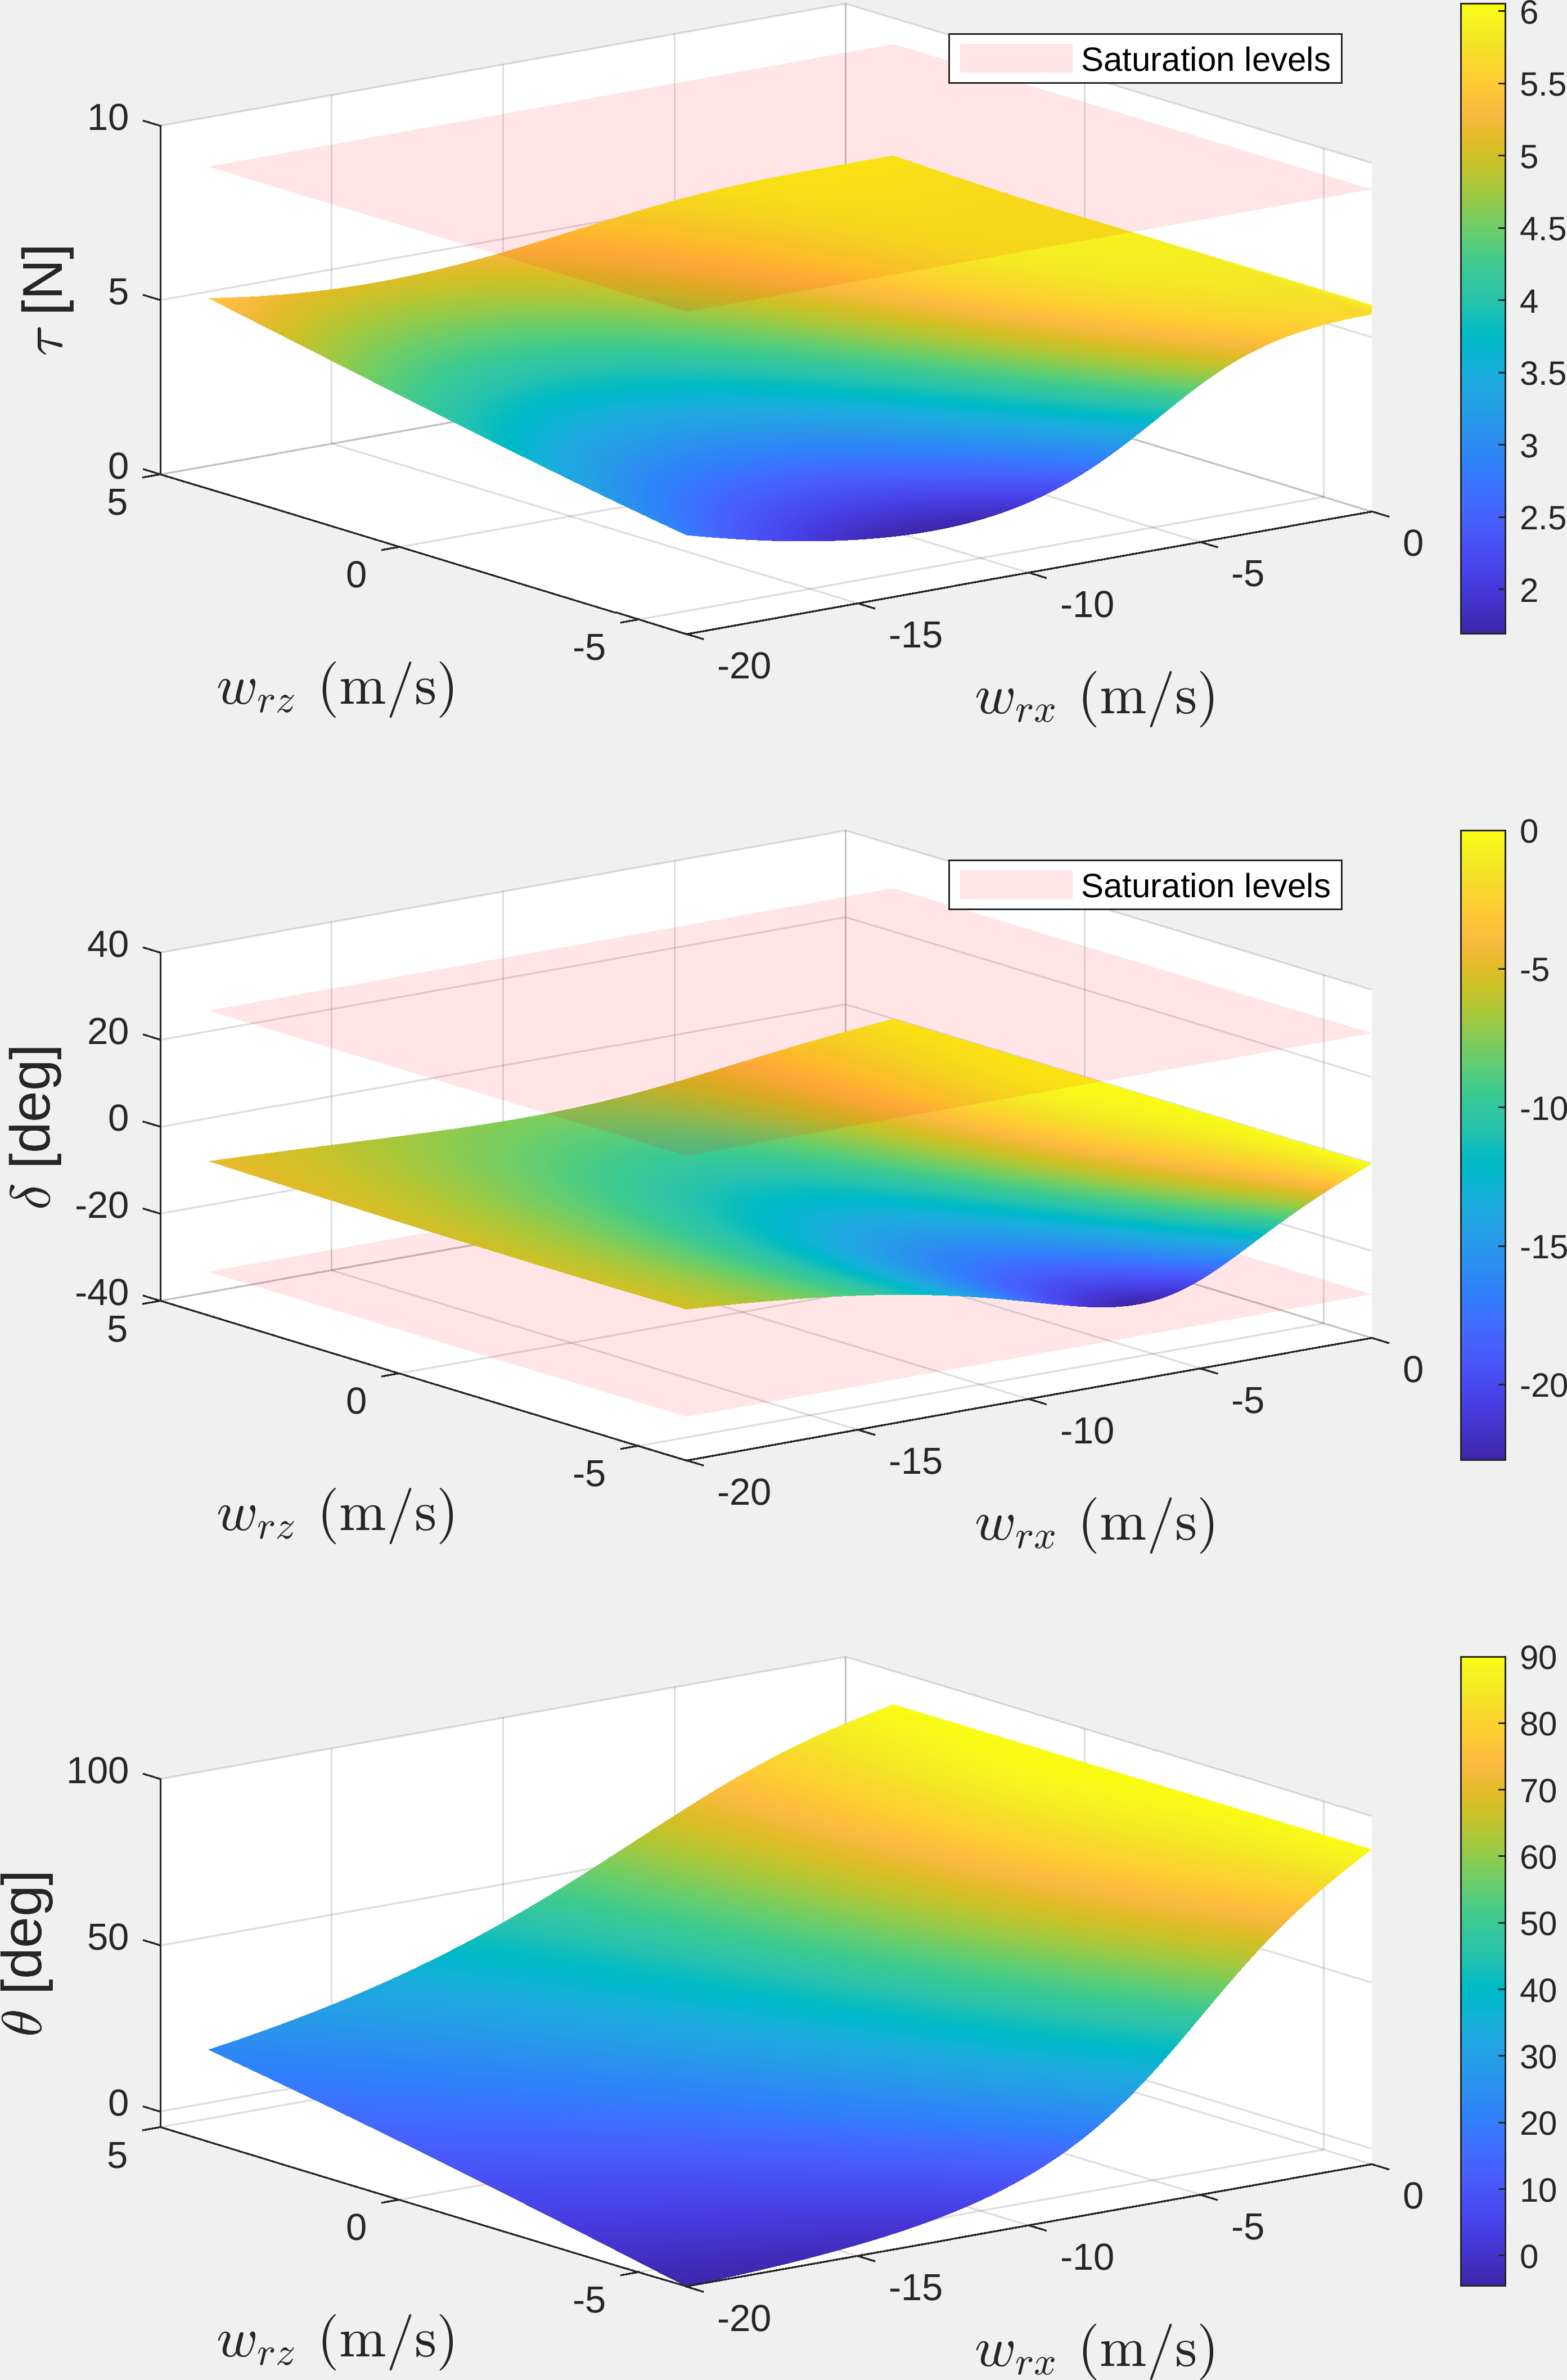
\includegraphics[trim=0cm 0cm 0cm 0cm,clip,width=0.5\columnwidth]{figures/equilibrium_wx_wz.png}
        \caption{Les paramètres ($\tau$, $\delta$, $\theta$) de l'ensemble des points d'équilibres (surface) obtenue à l'aide du Théorème~\ref{thm:eqs} et de l'Algorithme \ref{alg:eq} pour un vent constant horizontal et vertical ($w_{\text{r}x}$,$w_{\text{r}z}$), avec les saturations des actionneurs (rose).}
        \label{fig:saturation}
    \end{figure}
    Il est possible de faire une coupe des surfaces présentée dans \eqref{fig:saturation} pour une vitesse verticale nulle $\boldsymbol{w}_{\text{rx}} = 0$, ce qui nous donne le résultat de la Figure \ref{fig:saturation_wz0}
    \begin{figure}[ht!]
        \centering
        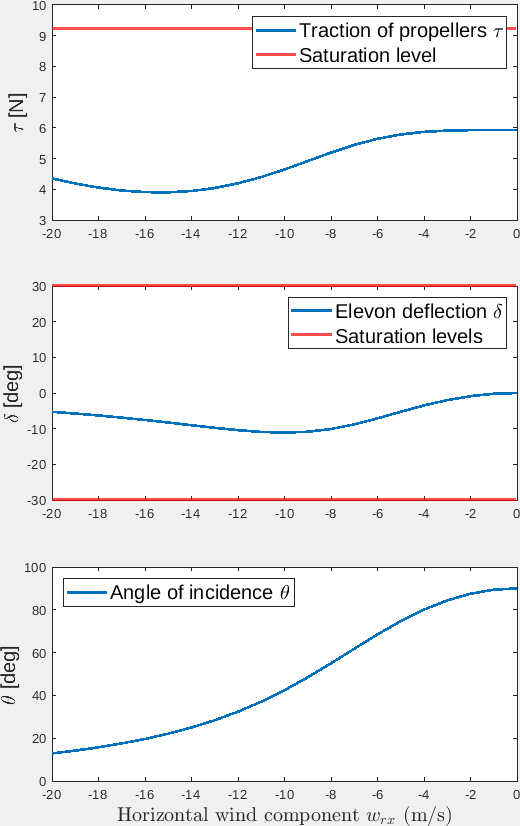
\includegraphics[trim=0cm 0cm 0cm 0cm,clip,width=0.5\columnwidth]{figures/equilibrium.png}
        \caption{Section des surfaces de la Figure \ref{fig:saturation} pour $w_{\text{r}z} = \SI{0}{\meter\per\second}$.}
        \label{fig:saturation_wz0}
    \end{figure}

\section{Dynamiques linéarisés}
\subsection{Dynamique linéarisé sans vent}
Considérons le cas sans vent discuté dans la section \ref{sec:eq_nowind} pour lequel nous utilisons le vecteur de commande $\boldsymbol{u}_{\text{nowind}}$  et le vecteur de commande à l'équilibre $\boldsymbol{u}_{\text{nowind},\text{eq}}$ défini dans l'équation \eqref{eq:bar_u} et rappelons la transformation du vecteur de commande suivante $ \boldsymbol{u}_{\text{nowind}} := \begin{bmatrix}\tau_{1}  \!&\! \tau_{2}  \!&\! \delta_{1}\tau_{1} \!&\! \delta_{2}\tau_{2} \end{bmatrix}^\top$, la dynamique linéarisé dans le cas sans vent est 
\begin{align}
    \label{eq:linearized}
     \boldsymbol{\dot{\tilde{x}}} = \boldsymbol{A}_{0} \tilde{\boldsymbol{x}} + \boldsymbol{G}_{0} (\boldsymbol{u}_{\text{nowind}}-\boldsymbol{u}_{\text{nowind},\text{eq}}),
\end{align}
où l'expression de $\boldsymbol{A}_{0}$ est
\begin{align}
    \label{matrice_A}
        \boldsymbol{A}_{0} = \boldsymbol{A}_{w} \Big|_{\boldsymbol{w}=0} =\begin{bmatrix}
        \mathbb{0}_{3} & \mathbb{I}_{3} & \mathbb{0}_{3} & \mathbb{0}_{3} \\
        \mathbb{0}_{3} & \mathbb{0}_{3} &  \boldsymbol{A}_{v\epsilon} & \mathbb{0}_{3} \\
        \mathbb{0}_{3} & \mathbb{0}_{3} & \mathbb{0}_{3} & \boldsymbol{A}_{\epsilon\omega} \\
        \mathbb{0}_{3} & \mathbb{0}_{3} & \mathbb{0}_{3} & \mathbb{0}_{3}
        \end{bmatrix},
\end{align}
avec les matrices suivantes
\begin{align*}
    \boldsymbol{A}_{\epsilon\omega} = \frac{\sqrt{2}}{4}\begin{bmatrix} 
        1 & 0 & -1 \\ 
        0 & 1 & 0  \\
       1 & 0 & 1
    \end{bmatrix} \text{ et } \boldsymbol{A}_{ v\epsilon} = \sqrt{2}\begin{bmatrix} 
        0 & -2g & 0\\
        g & 0 & g  \\ 
         0 & -2g & 0 \end{bmatrix},
\end{align*}
alors que l'expression de $\boldsymbol{G}_{0}$ est
\begin{align*}
    \boldsymbol{G}_{0}  := \begin{bmatrix}
    \mathbb{0}_{3\times 1} & \mathbb{0}_{3\times 1} & \mathbb{0}_{3\times 1} & \mathbb{0}_{3\times 1}\\
    0 & 0 & a_{\text{g}} & a_{\text{g}}\\
    0 & 0 & 0 & 0\\
    b_{\text{g}} & b_{\text{g}}  & 0 & 0\\
    \mathbb{0}_{3\times 1} & \mathbb{0}_{3\times 1} & \mathbb{0}_{3\times 1} & \mathbb{0}_{3\times 1}\\
    c_{\text{g}} & -c_{\text{g}} & d_{\text{g}} & -d_{\text{g}}\\
    0 & 0 & e_{\text{g}} & e_{\text{g}}\\
    f_{\text{g}} & -f_{\text{g}} & 0 & 0\\
    \end{bmatrix} , 
\end{align*}
avec
\begin{align*}
    \left[\!\! \begin{array}{c|c} 
    a_{\text{g}} & b_{\text{g}} \\ \hline
    c_{\text{g}} & d_{\text{g}} \\ \hline
    e_{\text{g}} & f_{\text{g}}
    \end{array} \!\!\right] \!=\!
    \left[\begin{array}{c|c}
   \shortminus \frac{S_{\text{wet}}}{4mS_{\text{p}}}C_{\ell}\xi_{\text{f}}  & \frac{1}{m}( 1-\frac{S_{\text{wet}}}{2S_{\text{p}}} C_{\text{d}}) \\ \hline
    \frac{k_{\text{m}} }{J_{x}k_{\text{f}}}  &   \! \frac{ S_{\text{wet}} a_{y} }{4 J_{x} S_{\text{p}} } C_{\ell}\xi_{\text{f}} \!\\ \hline
    \!\! \frac{S_{\text{wet}}\Delta_{\text{r}}}{4J_{y}S_{\text{p}}} C_{\ell}\xi_{\text{m}} \!\! & 
    \frac{1}{J_{z}}(p_{y}\!+\!\frac{S_{\text{wet}}}{4S_{\text{p}}} a_{y} C_{\text{d}})\!\!
    \end{array}\right].
\end{align*}

\subsection{Dynamique linéarisé en présence de vent}

Pour chacun des équilibres caractérisés dans le Théorème~\ref{thm:eqs}, nous détaillons les équations linéarisées du mouvement par rapport au modèle non linéaire simplifié à faible vitesse \eqref{eq:dyna_simp}. Une approche directe conduirait à des équations linéarisées qui dépendent de l'angle $\psi$ caractérisé à l'étape 1 de l'Algorithme~\ref{alg:eq}. Au lieu de cela, nous définissons ici les coordonnées incrémentales dans un cadre de référence inertiel convenablement tourné, de sorte que la dynamique linéarisée soit indépendante de l'angle $\psi$.
Plus précisément, pour chaque condition de vent d'équilibre $\boldsymbol{w}_{\text{eq}}$ associé à l'équilibre $(\boldsymbol{u}_{\text{eq}}, \boldsymbol{p}_{\text{eq}},\boldsymbol{v}_{\text{eq}}, \boldsymbol{q}_{\text{eq}},\boldsymbol{\omega}_{\text{b},\text{eq}})$  caractérisé en \eqref{eq:qpsi}--\eqref{eq:qtheta}, 
désignant les composantes scalaire et vectorielle du quaternion en \eqref{eq:qeq} comme
$\boldsymbol{q}_{\text{eq}} = (\eta_{\text{eq}}, \boldsymbol{\epsilon}_{\text{eq}})$, et à partir de la matrice de rotation
$\boldsymbol{R}_{\psi} :=    \boldsymbol{R}(\boldsymbol{q}_{\mathrm{eq}\psi})$ introduite au début de la preuve du Théorème~\ref{thm:eqs}, nous étudions ici la dynamique incrémental linéaire du vecteur d'état tourné :  
\begin{align}
\label{eq:xtilde}
     \nonumber &\tilde{\boldsymbol{x}} := (\tilde{\boldsymbol{p}},
     \tilde{\boldsymbol{v}},
     \tilde{\boldsymbol{\epsilon}},
     \tilde{\boldsymbol{\omega}}_{\text{b}}) = \left(\boldsymbol{R}^\top_{\psi} (\boldsymbol{p} \! \shortminus \! \boldsymbol{p}_{\text{eq}}), \boldsymbol{R}^\top_{\psi} \boldsymbol{v}, \boldsymbol{R}^\top_{\psi} (\boldsymbol{\epsilon} \! \shortminus \! \boldsymbol{\epsilon}_{\text{eq}}), \boldsymbol{\omega}_{\text{b}} \right), \\ &\tilde{\boldsymbol{u}} := \boldsymbol{u}-\boldsymbol{u_{\text{eq}}}, \quad \tilde{\boldsymbol{w}} := \boldsymbol{R}^\top_{\psi} (\boldsymbol{w}-\boldsymbol{w}_{\mathrm{eq}}).
\end{align}
Notez que la rotation en \eqref{eq:xtilde} possède la propriété $\boldsymbol{R}^\top_{\psi} \boldsymbol{\epsilon}_{\text{eq}} = \smallmat{0 & \sin(\frac{\theta}{2}) & 0}^\top$, ce qui simplifie grandement le mouvement linéarisé.

En exploitant le fait que les vitesses lineaaire et angulaire ($\boldsymbol{v}_{\text{eq}}$, $\boldsymbol{\omega}_{\text{b,eq}})$ doit être nulle à l'équilibre (voir \eqref{eq:equilibrium}), nous prouvons ci-dessous que la dynamique linéarisée de l'état \eqref{eq:xtilde} est donnée par
\begin{align}
\label{eq:lpv_linearisation}
 \boldsymbol{\dot{\tilde{x}}} &= \boldsymbol{A}_{w} \tilde{\boldsymbol{x}} + \boldsymbol{G}_{w} \tilde{\boldsymbol{u}} + \boldsymbol{E}_{w}  \tilde{\boldsymbol{w}} \\
 &= \smallmat{
     \mathbb{0}_{3} & \mathbb{I}_{3} & \mathbb{0}_{3} &\mathbb{0}_{3} \\
    \mathbb{0}_{3} & \boldsymbol{A}_{vv}  & \boldsymbol{A}_{v\epsilon}  & \mathbb{0}_{3}\\
    \mathbb{0}_{3} & \mathbb{0}_{3} & \mathbb{0}_{3} & \boldsymbol{A}_{\epsilon \omega} \\    
    \mathbb{0}_{3} & \mathbb{0}_{3} &  \boldsymbol{A}_{\omega \epsilon} & \mathbb{0}_{3}
    } \tilde{\boldsymbol{x}} \!+\!
    \smallmat{ \mathbb{0}_{3 \times 4} \\
     \boldsymbol{G}_{v}\\
     \mathbb{0}_{3 \times 4}\\
     \boldsymbol{G}_{\omega}
    } \tilde{\boldsymbol{u}}
    \!+\! \smallmat{
     \mathbb{0}_{3 \times 3} \\
     \boldsymbol{E}_{v} \\
     \mathbb{0}_{3 \times 3} \\
     \boldsymbol{E}_{\omega} 
     } \!\tilde{\boldsymbol{w}},
     \nonumber
\end{align}
%
avec les matrices $\boldsymbol{A}_{vv} $, $\boldsymbol{A}_{v\epsilon}$, $\boldsymbol{A}_{\epsilon \omega_{\text{b}}}$, $\boldsymbol{A}_{\omega \epsilon}$, $ \boldsymbol{G}_{v}$, $\boldsymbol{G}_{\omega}$ $\boldsymbol{E}_{v}$, $\boldsymbol{E}_{\omega}$ construite en suivant l'Algorithme~\ref{alg:linea}.

\begin{theorem} \label{th:lin}
Pour tout vent constant, $\boldsymbol{w} =\smallmat{w_x & w_y & w_z}^\top \in \real^3$ ayant une composante horizontale non nulle $\smallmat{w_x \\ w_y}$, et le doublet d'équilibre qui découle $(\boldsymbol{u}_{\text{eq}}, \boldsymbol{x}_{\text{eq}})$ de la dynamique \eqref{eq:dyna_simp}, tels que caractérisés dans \eqref{eq:qpsi}-\eqref{eq:qtheta}, la dynamique linéarisée du vecteur état incrémental \eqref{eq:xtilde} est donné par \eqref{eq:lpv_linearisation} avec les matrices construites comme dans l'Algorithme~\ref{alg:linea}.
\end{theorem}
%
\begin{proof}
Tout d'abord, en exploitant la matrice de rotation 
$\boldsymbol{R}_{\psi} :=    \boldsymbol{R}(\boldsymbol{q}_{\mathrm{eq}\psi})$ utilisé dans \eqref{eq:xtilde}, nous transformons la dynamique non linéaire \eqref{eq:dyna_simp} en coordonnées tournées
\begin{align}
\label{eq:rotated_coord}
(\boldsymbol{p}_{\text{r}} ,
\boldsymbol{v}_{\text{r}} ,
\boldsymbol{q}_{\text{r}}
)
:=
\left(\boldsymbol{R}_{\psi}^\top
\boldsymbol{p},
\boldsymbol{R}_{\psi}^\top \boldsymbol{v},
\boldsymbol{q}_{\mathrm{eq}\psi}^{-1} \otimes
\boldsymbol{q}
\right), 
\; \boldsymbol{w}_{\text{r}}:=\boldsymbol{R}_{\psi}^\top\boldsymbol{w}
\end{align}
où $\boldsymbol{\omega}_{\text{b}}$ reste inchangée car elle est exprimée dans le repère du corps. 
Quelques observations permettent de simplifier
la dynamique transformée \eqref{eq:dyna_simp}:
\begin{itemize}
    \item nous avons $\boldsymbol{R}_{\psi}^\top
    m\boldsymbol{g} = m\boldsymbol{g}$ car la rotation de $\psi$ est autour de l'axe $z_{[\text{i}]}$;
    \item comme $\boldsymbol{q}_{\text{r}} = \boldsymbol{q}_{\mathrm{eq}\psi}^{-1} \otimes \boldsymbol{q}$, alors $\boldsymbol{R}_{\psi}^\top \boldsymbol{R}(\boldsymbol{q}) = \boldsymbol{R}(\boldsymbol{q}_{\text{r}})$; 
    \item comme $\boldsymbol{v}_{\text{b}} := \boldsymbol{R}^\top(\boldsymbol{q}) (\boldsymbol{v}-\boldsymbol{w})$ (comme défini après l'équation \eqref{eq:Mb}), alors $\| \boldsymbol{v}_{\text{b}} \| = \| \boldsymbol{v} -  \boldsymbol{w}  \| - \| \boldsymbol{v}_{\text{r}} -  \boldsymbol{w}_{\text{r}}  \|$
    \item enfin $\boldsymbol{R}^\top(\boldsymbol{q}) \boldsymbol{w} = \boldsymbol{R}^\top\! (\boldsymbol{q}_{\text{r}}) \boldsymbol{R}_{\psi}^\top\! \boldsymbol{R}_{\psi} \boldsymbol{w}_{\text{r}}= \boldsymbol{R}^\top \!(\boldsymbol{q}_{\text{r}}) \boldsymbol{w}_{\text{r}}$.
\end{itemize} 

Sur la base des observations ci-dessus, nous pouvons dériver la version tournée des équations \eqref{eq:dyna_simp} comme étant
\begin{subequations}\label{eq:dyna_simp_rot}
    \begin{alignat}{3}
        \boldsymbol{\dot p}_{\text{r}} &=  \boldsymbol{v}_{\text{r}}, \label{eq:p_r} \\
        m \boldsymbol{\dot v}_{\mathrm{r}} &= \!\shortminus m\boldsymbol{g} \!+ \! \boldsymbol{R}(\boldsymbol{q}_{\mathrm{r}})\left(\boldsymbol{M}_{\text{f}}(\boldsymbol{u}) \! + \! \boldsymbol{D}_{\text{f}}(\boldsymbol{u}) \lVert \boldsymbol{w}_{\text{r}} \rVert \boldsymbol{R}^\top \!(\boldsymbol{q}_{\mathrm{r}}) (\boldsymbol{v}_{\mathrm{r}} \! \shortminus \! \boldsymbol{w}_{\text{r}}) \right),  \label{eq:v_r} \\
       \boldsymbol{\dot{q}}_{\text{r}} &=  \left( \frac{1}{2}\boldsymbol{q}_{\text{r}} \otimes \smallmat{0 \\ \boldsymbol{\omega}_{\text{b}}} \right),  \label{eq:q_r}\\
        \boldsymbol{J} \boldsymbol{\dot \omega}_{\text{b}} &=   \shortminus \skewsym{\boldsymbol{\omega}_{\text{b}}}\boldsymbol{J}\boldsymbol{\omega}_{\text{b}}\! + \boldsymbol{M}_{\text{m}}(\boldsymbol{u}) \! + \! \boldsymbol{D}_{\text{m}} (\boldsymbol{u}) \lVert  \boldsymbol{w}_{\text{r}} \rVert \boldsymbol{R}^\top \!(\boldsymbol{q}_{\mathrm{r}}) (\boldsymbol{v}_{\mathrm{r}} \! \shortminus \! \boldsymbol{w}_{\text{r}})  
        \label{eq:w_r}
    \end{alignat}
\end{subequations}
Avec ces nouvelles coordonnées, les vecteurs d'état incrémental \eqref{eq:xtilde} peut être exprimés comme étant
\begin{align}
\label{eq:xtilde_rot}
     \nonumber &\tilde{\boldsymbol{x}} = \left(
     \boldsymbol{p}_{\text{r}} \! \shortminus \!  \boldsymbol{R}^\top_{\psi}\boldsymbol{p}_{\text{eq}}, \boldsymbol{v}_{\text{r}},  
     \boldsymbol{\epsilon}_{\text{r}} \! \shortminus \! \boldsymbol{R}^\top_{\psi}\boldsymbol{\epsilon}_{\text{eq}}, \boldsymbol{\omega}_{\text{b}} \right), \\ &\tilde{\boldsymbol{u}} := \boldsymbol{u}-\boldsymbol{u_{\text{eq}}}, \quad \tilde{\boldsymbol{w}} :=  \boldsymbol{w}_{\mathrm{r}}-\boldsymbol{w}_{\mathrm{r,eq}}
\end{align}
où $\boldsymbol{w}_{\mathrm{r,eq}} = \boldsymbol{R}^\top_{\psi}\boldsymbol{w}_{\mathrm{eq}} = \smallmat{w_{\text{r}x} \\ 0 \\w_{\text{r}z}}$, déjà défini dans \eqref{eq:wh}, et $\boldsymbol{R}^\top_{\psi} \boldsymbol{\epsilon}_{\text{eq}} = \smallmat{0 & \sin(\frac{\theta}{2}) & 0}^\top$ ont tous deux une structure peu dense intéressante.


En se concentrant sur la dynamique tournée \eqref{eq:dyna_simp_rot} et l'expression \eqref{eq:xtilde_rot} des variables incrémentales, la preuve du théorème revient à montrer que la linéarisation de \eqref{eq:dyna_simp_rot} autour de
l'équilibre tourné
\begin{align}
\label{eq:rotated_eq}
\boldsymbol{x}_{\text{r,eq}} &= \left( \boldsymbol{p}_{\text{r,eq}}, \boldsymbol{v}_{\text{r,eq}},
\boldsymbol{\epsilon}_{\text{r,eq}},
\boldsymbol{\omega}_{\text{br,eq}} \right) \\
\nonumber
&= \left(\boldsymbol{R}^\top_{\psi} \boldsymbol{p}_{\text{eq}},  
\smallmat{0 \\ 0 \\ 0},   \smallmat{0 \\ \sin(\frac{\theta}{2}) \\ 0}, 
\smallmat{0 \\ 0 \\ 0} \right),\;
\boldsymbol{w}_{\mathrm{r,eq}}  = \smallmat{w_{\text{r}x} \\ 0 \\w_{\text{r}z}}
\end{align}
coïncide avec l'équation \eqref{eq:lpv_linearisation} et les expressions de l'Algorithme~\ref{alg:linea}.

Dans ce but, inspirée par \cite[Proof of Lemma 1]{tregouetHal-01760720}, pour linéariser la dynamique du quaternion $\boldsymbol{q}_{\text{r}} = \left[ \eta_{\text{r}} ~ \boldsymbol{\epsilon}_{\text{r}}^\top \right]^\top$ évoluant dans ${\mathbb S}^3$, nous remplaçons  $\eta_{\text{r}}$ par sa valeur positive lié à la norme unitaire du quaternion. Ainsi, $\eta_{\text{r}} = (1- \boldsymbol{\epsilon}_{\text{r}}^\top \boldsymbol{\epsilon}_{\text{r}})^\frac{1}{2}$.
Concentrons-nous d'abord sur la matrice $\boldsymbol{A}_w$ dans \eqref{eq:lpv_linearisation}. Les trois premières lignes sont simplement $\smallmat{\mathbb{0}_{3} & \mathbb{I}_{3} & \mathbb{0}_{3} &\mathbb{0}_{3}}$, du fait de la linéarité de l'équation \eqref{eq:p_r}. 
Pour le second bloc de ligne, nous nous concentrons sur l'équation \eqref{eq:v_r} et nous commençons par caractériser $\boldsymbol{R}(\boldsymbol{q}_{\mathrm{r,eq}})$, dont la structure est relativement vide de $\boldsymbol{\epsilon}_{\text{r,eq}}$. En particulier, nous rappelons dans \eqref{eq:wb} en utilisant l'expression $\boldsymbol{R}$ dans \eqref{eq:matrix_rot}, nous pouvons écrire
\begin{align*}
    \boldsymbol{R}(\boldsymbol{q}_{\mathrm{r,eq}\textbf{}})= \boldsymbol{R}_\theta :=
     \begin{bmatrix}1-2\overline \epsilon_{2}^{2} & 0 & 2\overline\epsilon_{2} \overline{\eta} \\ 0 & 1 & 0 \\ -2\overline\epsilon_{2} \overline{\eta} & 0 & 1-2\overline\epsilon_{2}^{2} \end{bmatrix}
    = \smallmat{ \cos \theta & 0 & \sin \theta \\ 0 & 1 & 0 \\ -\sin \theta & 0 & \cos \theta },
\end{align*}
où $\overline \epsilon_{2} = \sin{\frac{\theta}{2}}$ représente le deuxième élément de $\boldsymbol{\epsilon}_{\text{r,eq}}$ selon \eqref{eq:rotated_eq} et $ \overline{\eta} = \sqrt{1-\overline \epsilon_{2}^{2}} = \cos{\frac{\theta}{2}}$.

Avec cette expression de $ \boldsymbol{R}_\theta$, nous pouvons dériver l'expression de \eqref{eq:v_r}, en utilisant la notation abrégée $\left. \cdot \right|_{\text{eq}}$ pour caractériser l'évaluation d'une fonction (matricielle ou vectorielle) à l'équilibre \eqref{eq:rotated_eq},
\begin{align}
\nonumber
\boldsymbol{A}_{vv} &\!=\! \frac{\partial }{\partial \boldsymbol{v}}  \left. \left( \frac{1}{m} \boldsymbol{R}(\boldsymbol{q}_{\text{r}}) \left( %\boldsymbol{M}_{\text{f}}(\boldsymbol{u}) +  
\boldsymbol{D}_{\text{f}}(\boldsymbol{u}) \lVert \boldsymbol{w}_{\text{r}} \rVert \boldsymbol{R}^\top \!(\boldsymbol{q}_{\mathrm{r}}) ( \boldsymbol{v}_{\mathrm{r}} \! \shortminus \! \boldsymbol{w}_{\text{r}})  \right) \right)\right|_{\text{eq}}\\
&\!=\!  \left. \frac{\partial }{\partial \boldsymbol{v}} \left( \frac{1}{m}  \boldsymbol{R}_\theta  \boldsymbol{D}_{\text{f}}(\boldsymbol{u_{\text{eq}}}) \lVert \boldsymbol{w}_{\mathrm{eq}} \rVert   \boldsymbol{R}_\theta^\top  \boldsymbol{v}_{\mathrm{r}} \right) \right|_{\text{eq}},
\label{eq:Avv_derivation}
\end{align} 
qui, compte tenu de l'égalité $\boldsymbol{D}_{\text{f,eq}} = \boldsymbol{D}_{\text{f}}(\boldsymbol{u_{\text{eq}}})$, il est facile de montrer qu'elle coïncide avec la matrice
$\boldsymbol{A}_{vv}$ donnée en \eqref{eq:Avv_alg2} dans l'Algorithme~\ref{alg:linea}.

Nous nous concentrons maintenant sur $\boldsymbol{A}_{v\epsilon}$ de la matrice 
$\boldsymbol{A}_{w}$,  qui doit être calculée à partir de \eqref{eq:v_r} de manière similaire à
\eqref{eq:Avv_derivation}, comme
\begin{align}
\boldsymbol{A}_{v\epsilon} &\!=\! \frac{\partial }{\partial \boldsymbol{\epsilon}}  \left. \left( \frac{1}{m} \boldsymbol{R}(\boldsymbol{q}_{\text{r}}) \left( 
\boldsymbol{M}_{\text{f}}(\boldsymbol{u}) +  
\boldsymbol{D}_{\text{f}}(\boldsymbol{u}) \lVert \boldsymbol{w}_{\text{r}} \rVert \boldsymbol{R}^\top \!(\boldsymbol{q}_{\mathrm{r}}) \boldsymbol{w}_{\text{r}}  \right) \right)\right|_{\text{eq}}.
\label{eq:Aveps_derivation}
\end{align} 
Pour évaluer la partie droite de \eqref{eq:Aveps_derivation}, nous demmarons de l'expression de $\boldsymbol{R}(\boldsymbol{q}) = \boldsymbol{R}\left( \smallmat{\eta \\ \epsilon}\right)$ dans \eqref{eq:matrix_rot}, après la substitution de 
$\eta = \sqrt{1-\boldsymbol{\epsilon}^\top \boldsymbol{\epsilon}} \neq 0$
(nous rappelons que pour tous les équilibres caractérisés, nous avons $\eta \neq 0$), nous pouvons calculer la dérivée généralisée
\begin{align}
\label{eq:diffR_eps}
&\partial \boldsymbol{R}_{\boldsymbol{ \epsilon}} (\boldsymbol{ \epsilon},\mathfrak{v}) := \frac{\partial }{\partial \boldsymbol{\epsilon}}
\boldsymbol{R}\left(
\smallmat{\sqrt{1-\boldsymbol{\epsilon}^\top \boldsymbol{\epsilon}} \\ \boldsymbol{\epsilon}}
\right) \mathfrak{v}  \\
\nonumber
&\; = 2 \eta \skewsym{\mathfrak{v}} \left( \frac{\boldsymbol{\epsilon}\boldsymbol{\epsilon}^\top}{1-\boldsymbol{\epsilon}^\top \boldsymbol{\epsilon}} - \mathbb{I}_{3}  \right) \shortminus 4 \mathfrak{v} \boldsymbol{\epsilon}^\top \! + \!2\boldsymbol{\epsilon} \mathfrak{v}^\top \!+ \! 2\boldsymbol{\epsilon}^\top \mathfrak{v} \mathbb{I}_{3},
\end{align}
qui implique donc
\begin{align}
\label{eq:diffRtop}
    \frac{\partial }{\partial \boldsymbol{\epsilon}}
\boldsymbol{R}^\top\left(
\smallmat{\eta \\ \boldsymbol{\epsilon}}
\right) \mathfrak{v} =
    \frac{\partial }{\partial \boldsymbol{\epsilon}}
\boldsymbol{R}\left(
\smallmat{\sqrt{1-\boldsymbol{\epsilon}^\top \boldsymbol{\epsilon}} \\ -\boldsymbol{\epsilon}}
\right) \mathfrak{v} = \partial \boldsymbol{R}_{\boldsymbol{ \epsilon}} (\boldsymbol{ -\epsilon},\mathfrak{v}).
\end{align}
Pour évaluer \eqref{eq:Aveps_derivation}, il sera utile de dériver la forme simplifiée suivante
\begin{align}
\label{eq:diffRsparse}
    &\partial \boldsymbol{R}_{\boldsymbol{ \epsilon}} \left(
    \smallmat{0 \\ \epsilon_2 \\ 0}
    ,\smallmat{\mathfrak{v}_1 \\ 0 \\ \mathfrak{v}_3}\right) \nonumber \\ 
    & = 2  \smallmat{0 & \left( \overline{\eta} - \frac{\overline \epsilon_{2}^{2}}{\overline{\eta}} \right) \mathfrak{v}_3 & 0\\
    -\overline{\eta} \mathfrak{v}_3 & 0 & \overline{\eta} \mathfrak{v}_1 \\
    0 & \left( \frac{\overline \epsilon_{2}^{2}}{\overline{\eta}} - \overline{\eta} \right) \mathfrak{v}_1 & 0} + 2\overline \epsilon_{2}\smallmat{ 0 & -2\mathfrak{v}_1 & 0\\
    \mathfrak{v}_1 & 0 & \mathfrak{v}_3 \\
    0 & -2\mathfrak{v}_3 & 0}.
\end{align}

Nous pouvons définir deux forces $(f_{\text{d}} , f_{\ell})$ qui agissent sur le drone à l'équilibre, exprimées dans le repère corps, et qui dépendent du vent $\boldsymbol{w}$ et des deux entrées similaires des élevons $\delta$. Ces deux forces sont la traînée et la portance générées par l'écoulement de l'air sur l'aile. Elles résultent du développement de l'expression $ \boldsymbol{D}_{\text{f}}(\boldsymbol{u}) \lVert \boldsymbol{v}_{\text{b}} \rVert \boldsymbol{v}_{\text{b}}$ provenant \eqref{eq:v_r} avec $\boldsymbol{D}_{\text{f}}(\boldsymbol{u})$ De \eqref{eq:df}:
\begin{align}
\label{eq:draglift}
    \smallmat{f_{\text{d}} \\ 0 \\ f_{\ell}} = - \boldsymbol{D}_{\text{f}}(\boldsymbol{u_{\text{eq}}}) \lVert \boldsymbol{w}_{\mathrm{eq}} \rVert  \boldsymbol{R}_\theta^\top \boldsymbol{w}_{\mathrm{r,eq}},
\end{align}
qui après calcul coïncide avec l'expression \eqref{eq:draglift_ALG} donner dans l'Algorithme~\ref{alg:linea}. 

À partir des deux forces $(f_{\text{d}} , f_{\ell})$ dans \eqref{eq:draglift}, il est possible de déterminer leurs dérivées partielles par rapport à la composante $\overline \epsilon_2$ du quaternion, qui représente le tangage du drone. En utilisant \eqref{eq:diffRtop}, nous obtenons
\begin{align}
    \smallmat{\frac{\partial  f_{\text{d}}  }{\partial \epsilon_{2}} \\ 0 \\ \frac{\partial  f_{\ell}  }{\partial \epsilon_{2}}} = - \boldsymbol{D}_{\text{f}}(\boldsymbol{u_{\text{eq}}})  \lVert \boldsymbol{w}_{\mathrm{eq}} \rVert \partial \boldsymbol{R}_{\boldsymbol{ \epsilon}}( -\boldsymbol{ \epsilon}, \boldsymbol{w}_{\mathrm{r,eq}}) \smallmat{0\\ 1\\ 0},
\end{align}
qui après calcul en utilisant l'égalité $\boldsymbol{D}_{\text{f,eq}} = \boldsymbol{D}_{\text{f}}(\boldsymbol{u_{\text{eq}}})$,
coïncide avec l'équation \eqref{eq:draglift_ALG}, donné dans l'Algorithme~\ref{alg:linea}.

En suivant des calculs similaires,  la force
$f_{\text{m}}$ générée par les moteurs, liée à la traction des hélices et à la traînée générée par l'écoulement de l'air sur l'aile, et la force $f_{\text{e}}$ générée par les élevons, liée à l'écoulement de l'air créé par les hélices, sont obtenues à partir de \eqref{eq:Mf} sont défini par 
\begin{align}
\label{eq:motor_el}
    \smallmat{ f_{\text{m}}  \\ 0 \\ f_{\text{e}} } &= \boldsymbol{M}_{\text{f}}(\boldsymbol{u_{\text{eq}}}) ,
\end{align}
qui, après calculs, coïncident avec les sélections de \eqref{eq:motor_elevon_forces}, données dans l'Algorithme~\ref{alg:linea}.

En utilisant les définitions \eqref{eq:diffR_eps}, \eqref{eq:diffRtop}, ainsi que les expressions \eqref{eq:diffRsparse}, \eqref{eq:draglift}, \eqref{eq:motor_el}, et leurs formes équivalentes indiquées dans \eqref{eq:draglift_ALG}, \eqref{eq:motor_elevon_forces} données dans l'Algorithme~\ref{alg:linea}, nous pouvons finalement calculer à partir de \eqref{eq:Aveps_derivation}
\begin{multline*}
    \!\boldsymbol{A}_{v\epsilon} \!=\! \frac{1}{m} \big( \partial \boldsymbol{R}_{\boldsymbol{ \epsilon}} (\boldsymbol{ \epsilon} , \boldsymbol{M}_{\text{f}}(\boldsymbol{u_{\text{eq}}}))  \shortminus \partial \boldsymbol{R}_{\boldsymbol{ \epsilon}} ( \boldsymbol{ \epsilon} ,\boldsymbol{D}_{\text{f}}(\boldsymbol{u_{\text{eq}}})  \lVert \boldsymbol{w}_{\mathrm{eq}} \rVert  \boldsymbol{R}_\theta^\top \! \boldsymbol{w}_{\mathrm{eq}})  \\    \left. \shortminus  \boldsymbol{R}_\theta \boldsymbol{D}_{\text{f}}(\boldsymbol{u})  \lVert \boldsymbol{w}_{\mathrm{r,eq}} \rVert \partial \boldsymbol{R}_{\boldsymbol{ \epsilon}}( -\boldsymbol{ \epsilon}, \boldsymbol{w}_{\mathrm{r,eq}})\smallmat{0\\ 1\\ 0} \big)\right|_{\mathrm{eq}}.
\end{multline*}
qui fournit l'expression \eqref{eq:Aveps_derivation_ALG} dans l'Algorithme~\ref{alg:linea} après quelques calculs exploitant également $\boldsymbol{D}_{text{f,eq}} = \boldsymbol{D}_{text{f}}(\boldsymbol{u_{\text{eq}}})$.

Nous nous concentrons maintenant sur la matrice $\boldsymbol{A}_{\epsilon \omega}$ de  $\boldsymbol{A}_{w}$, et nous rappelons que, en raison des propriétés du produit de quaternion (voir, par exemple, \cite{hamel_minhduc}), 
$\smallmat{\eta \\ \boldsymbol{\epsilon}} \otimes \smallmat{0 \\ 
\boldsymbol{\omega}_{\mathrm{b}}} = 
\smallmat{ - \boldsymbol{\epsilon}^\top  \\ 
\eta \mathbb{I}_{3}   + [ \boldsymbol{\epsilon}]_{\times} 
} \boldsymbol{\omega}_{\mathrm{b}}$. 
À partir des deux termes inférieurs de la matrice du côté droit de cette dernière équation, en développant \eqref{eq:q_r}
et en calculant $\boldsymbol{A}_{\epsilon \omega} = \left. \frac{\partial }{\partial \boldsymbol{\omega}_{\text{b}}} \left( \frac{1}{2} \boldsymbol{{q}}_{\text{r}}  \otimes \smallmat{0 \\ \boldsymbol{\omega}_{\text{b}}} \right) \right|_{\mathrm{eq}}$,
nous obtenons les deux termes de l'expression \eqref{eq:Aveps_derivation_ALG} donnée dans l'Algorithme~\ref{alg:linea}.

Nous nous concentrons maintenant sur la matrice $\boldsymbol{A}_{\omega \epsilon}$ de $\boldsymbol{A}_{w}$, qui doit être calculée à partir de \eqref{eq:w_r}. Comme seul le dernier terme de la partie droite dépend de $\boldsymbol{\epsilon}$ (par l'intermédiaire de $\boldsymbol{q}_{\mathrm r}$), nous obtenons

\begin{align}
\label{eq:Aomega_eps_first}
\boldsymbol{A}_{ \omega \epsilon} =  \boldsymbol{J}^{-1}
\boldsymbol{D}_{\mathrm{m}} (\boldsymbol{u}_{\text{eq}}) \lVert  \boldsymbol{w}_{\mathrm{r}} \rVert 
\left. 
\frac{\partial }{\partial \boldsymbol{\epsilon}} \left( \boldsymbol{R}^\top \!(\boldsymbol{q}_{\mathrm{r}}) (\boldsymbol{v}_{\mathrm{r}} \! \shortminus \! \boldsymbol{w}_{\text{r}}) \right) \right|_{\mathrm{eq}}.
\end{align}
Pour calculer l'expression explicite de \eqref{eq:Aomega_eps_first}, nous exploitons à nouveau \eqref{eq:diffRtop} et \eqref{eq:diffRsparse}, et utilisons l'expression de $\boldsymbol{D}_{\mathrm{m}}$ dans \eqref{eq:dm}, ainsi que les identités $\overline \eta^2 - \overline \epsilon_2^2 = \cos \theta$ et $2\overline \eta \overline \epsilon_2^2 = \sin \theta$, qui fournissent, après quelques simplifications, l'expression \eqref{eq:ddotomega_deps}, donnée dans l'Algorithme~\ref{alg:linea}.

Passons maintenant à la dérivation des entrées de la matrice $\boldsymbol{G}_{w}$ dans \eqref{eq:lpv_linearisation}, dont les composantes peuvent être dérivées de \eqref{eq:v_r} et \eqref{eq:w_r}. En utilisant les quatre entrées de $\boldsymbol{u}$ dans \eqref{eq:vector_u}, et en se basant également sur la structure de $\boldsymbol{M}_{\text{f}}$,
$\boldsymbol{D}_{\text{f}}$, dans \eqref{eq:Mf}, \eqref{eq:df}, la forme explicite pour
\begin{align}
    \boldsymbol{G}_{v} \! &= \! 
    \frac{1}{m} \boldsymbol{R}_\theta \! \left.\frac{\partial}{\partial \boldsymbol{u}} \! 
     \left( \boldsymbol{M}_{\text{f}}(\boldsymbol{u}) \! - \! \boldsymbol{D}_{\text{f}}(\boldsymbol{u}) \lVert \boldsymbol{w}_{\text{r}} \rVert \boldsymbol{w}^{\text{b}}_{\mathrm{eq}}   \right)\right|_{\mathrm{eq}} ,
\end{align}
peut être calculée comme dans \eqref{eq:Gv_ALG_luca}, après quelques factorisations. 

De même, sur la base des matrices $\boldsymbol{M}_{\text{m}}$, $\boldsymbol{D}_{\text{m}}$ dans \eqref{eq:Mm}, \eqref{eq:dm}, 
nous pouvons calculer
\begin{align}
     \boldsymbol{G}_{\omega} \! &= \!  \boldsymbol{J}^{-1} \! \left.\frac{\partial}{\partial \boldsymbol{u}} \! 
     \left( \boldsymbol{M}_{\text{m}}(\boldsymbol{u}) \! - \! \boldsymbol{D}_{\text{m}}(\boldsymbol{u}) \lVert \boldsymbol{w}_{\text{r}} \rVert \boldsymbol{w}^{\text{b}}_{\mathrm{eq}}   \right)\right|_{\mathrm{eq}}
\end{align}
comme dans \eqref{eq:Gomega_ALG_Luca}, après quelques factorisations. 


Déterminons enfin l'expression de $\boldsymbol{E}_{v}$ dans \eqref{eq:lpv_linearisation}. Notons d'abord que nous pouvons écrire
$\|\boldsymbol{w}_\text{r}\| \boldsymbol{w}_\text{r} = 
 \boldsymbol{w}_\text{r} \sqrt{\boldsymbol{w}_\text{r}^\top \boldsymbol{w}_\text{r}  }$, de sorte que
$$
\frac{\partial }{\partial \boldsymbol{w}_\text{r}}
\|\boldsymbol{w}_\text{r}\| \boldsymbol{w}_\text{r} = 
\|\boldsymbol{w}_\text{r}\| \mathbb{I}_3
+ \frac{\boldsymbol{w}_\text{r} \boldsymbol{w}_\text{r}^\top}{\|\boldsymbol{w}_\text{r}\|} = 
\|\boldsymbol{w}_\text{r}\|
\left( \mathbb{I}_3 + \frac{\boldsymbol{w}_\text{r} \boldsymbol{w}_\text{r}^\top}{\boldsymbol{w}_\text{r}^\top \boldsymbol{w}_\text{r}} \right).
$$

À l'aide de \eqref{eq:v_r} et \eqref{eq:w_r} et de l'expression de $\boldsymbol{w}_\text{r}$ dans \eqref{eq:rotated_coord} et en suivant des calculs similaires aux cas précédents, nous obtenons l'expression
\eqref{eq:Ev_alg2} (indiquée dans l'Algorithme~\ref{alg:linea}), pour $\boldsymbol{E}_{v} = -  \frac{1}{m} \boldsymbol{R}_\theta \left. \frac{\partial}{\partial \boldsymbol{w}_\text{r}} \left(  \! \boldsymbol{D}_{\text{f}}(\boldsymbol{u}) \lVert \boldsymbol{w}_{\text{r}} \rVert \boldsymbol{w}_{\text{r}}  \right)\right|_{\mathrm{eq}} $ et  
 $\boldsymbol{E}_{w} = - \boldsymbol{J}^{-1} \left.
 \frac{\partial}{\partial \boldsymbol{w}_\text{r}} \left(  \boldsymbol{D}_{\text{m}}(\boldsymbol{u}) \lVert \boldsymbol{w}_{\text{r}} \rVert \boldsymbol{w}_{\text{r}}\right)\right|_{\mathrm{eq}}$, où nous rappelons que $\boldsymbol{D}_{\text{m,eq}} = \boldsymbol{D}_{\text{m}}(\boldsymbol{u_{\text{eq}}})$.
\end{proof}

\begin{algorithm}
     \caption{Détermination des matrices de la linéarisation de \eqref{eq:lpv_linearisation}}\label{alg:linea}
      \hspace*{.1cm} \textbf{Entrées} : Vecteur de vent $\boldsymbol{w}_{\text{eq}} =\smallmat{w_x & w_y & w_z}^\top$ et\\
      \hspace*{1.2cm} d'équilibre $(\boldsymbol{u}_{\text{eq}}, \boldsymbol{x}_{\text{eq}})$ provenant de \eqref{eq:equilibrium} et de l'Algorithme~\ref{alg:eq}.\\
 \hspace*{.1cm} \textbf{Sorties} : 
 Matrices $\boldsymbol{A}_{w}$, $\boldsymbol{G}_{w}$, $\boldsymbol{E}_{w}$ dans \eqref{eq:lpv_linearisation}

\begin{algorithmic}[1]

\State Sélectionner les paramètres $\psi$, $\theta$, $\tau$, $\delta$ de \eqref{eq:equilibrium} à l'aide de l'Algorithme~\ref{alg:eq} et de $\overline \epsilon_{2} = \sin{\frac{\theta}{2}}$, $\overline \eta =  \cos{\frac{\theta}{2}}$.

        
\State Avec les valeurs de \eqref{eq:wb}, \eqref{eq:df}, \eqref{eq:dm}, définissons : 
\begin{align*}
    & \boldsymbol{R}_\psi := \smallmat{ \cos \psi & \sin \psi & 0 \\ -\sin \psi & \cos \psi & 0 \\ 0 & 0 & 1 },    \quad 
      \boldsymbol{R}_\theta := \smallmat{ \cos \theta & 0 & \sin \theta \\ 0 & 1 & 0 \\ -\sin \theta & 0 & \cos \theta },         \\
     &\smallmat{w_{\text{r}x} \\ 0 \\ w_{\text{r}z}} :=  \boldsymbol{R}_\psi^\top \boldsymbol{w}_{\text{eq}}, \quad
    \smallmat{w^{\text{b}}_{x} \\ w^{\text{b}}_{z}} := \smallmat{w_{\text{r}x} \cos \theta -   w_{\text{r}z} \sin\theta \\ w_{\text{r}z} \cos \theta + w_{\text{r}x} \sin \theta }
     \\
     &\left[ \! \! \begin{array}{c|c} 
     \boldsymbol{D}_{\text{f,eq}} \! \! &  \! \! \boldsymbol{D}_{\text{m,eq}}
     \end{array} \! \!\right] \! \! := \! \! \frac{\rho S}{2} \left[\begin{array}{c|c} \! \! \begin{smallmatrix}
                \shortminus C_{\text{d}} & 0 & C_{\text{d}}\xi_{\text{f}} \delta\\
                0 & 0 & 0\\
                \shortminus C_{\ell}\xi_{\text{f}} \delta & 0 & \shortminus C_{\ell}
            \end{smallmatrix} &  \! \! \begin{smallmatrix}
                0 & 0 & 0\\
               \Delta_{\text{r}}C_{\ell}\xi_{\text{m}}\delta\ & 0 & 2\Delta_{\text{r}}C_{\ell}\\
                0 & 0 & 0
            \end{smallmatrix} \end{array} \! \!\right]
\end{align*}

\State Définissons les forces de portance et de trainé ainsi que leurs dérivées par rapport à $\epsilon_2$ (défini dans l'étape 1), comme
\begin{equation}
\label{eq:draglift_ALG}
\!\! \smallmat{\!f_{\text{d}} & \frac{\partial  f_{\text{d}}  }{\partial \epsilon_{2}} \!\! \\ 0 & 0  \\ \! f_{\ell} & \frac{\partial  f_{\ell} \!\! }{\partial \epsilon_{2}}} 
 \!\! := \! 
    \shortminus \| \boldsymbol{w}_{\mathrm{eq}} \|  \boldsymbol{D}_{\text{f,eq}}\! 
    \smallmat{\! w^{\text{b}}_{x} &  \left(\! 4 \overline{\eta}  \shortminus \frac{2\overline \epsilon_{2}^{2}}{\overline{\eta} } \! \right) w_{\text{r}z} \shortminus 8 \overline \epsilon_{2}  w_{\text{r}x} \!\! \\  0 & 0 \\  
   \! w^{\text{b}}_{z} &    \left(\! 4 \overline{\eta}  \shortminus \frac{2\overline \epsilon_{2}^{2}}{\overline{\eta} } \! \right) w_{\text{r}x} -8 \overline \epsilon_{2} w_{\text{r}z} \!\!
    }\!\!, 
\end{equation}

\State Définissons les forces des moteurs et des élevons comme
\begin{align}
\label{eq:motor_elevon_forces}
    \smallmat{ f_{\text{m}}  \\f_{\text{e}} }\! := \!\smallmat{\left(\frac{S_{\text{wet}}C_{\text{d}}}{2S_{\text{p}}}-2\right)\tau \\  - \frac{S_{\text{wet}}\tau \delta \xi_{\text{f}} C_{\ell}}{2S_{\text{p}}}}
\end{align}

\State Sélectionnons les matrices $\boldsymbol{A}_w$ dans \eqref{eq:lpv_linearisation} comme :
\begin{align}
\label{eq:Avv_alg2}
& \boldsymbol{A}_{vv} =
\frac{\| \boldsymbol{w}_{\mathrm{eq}} \| }{m} 
 \boldsymbol{R}_\theta \boldsymbol{D}_{\text{f,eq}}  \boldsymbol{R}_\theta^\top \\
\nonumber
&\smallmat{\boldsymbol{A}_{v\epsilon}^{1,2} \\ 
 \boldsymbol{A}_{v\epsilon}^{2,1} \\ \boldsymbol{A}_{v\epsilon}^{2,3} \\ \boldsymbol{A}_{v\epsilon}^{3,2}}
      := \smallmat{ 2 \overline{\eta}  - \frac{\overline \epsilon_{2}^{2}}{\overline{\eta} }  & 4 \overline \epsilon_{2} &  2\overline \epsilon_{2}^{2} -1 & 2\overline \epsilon_{2} \overline{\eta} \\
     -2 \overline{\eta}  & -2 \overline \epsilon_{2} & 0 & 0 \\ 
      2 \overline \epsilon_{2} & -2 \overline{\eta}  & 0 & 0 \\
      -4 \overline \epsilon_{2} & 2 \overline{\eta}  - \frac{\overline \epsilon_{2}^{2}}{\overline{\eta} } & -2\overline \epsilon_{2} \overline{\eta}  & 1- 2\overline \epsilon_{2}^{2}   }\smallmat{ f_{\text{e}}  + f_{\ell}  \\ f_{\text{m}}  + f_{\text{d}}  \\ \frac{\partial  f_{\text{d}}  }{\partial \overline \epsilon_{2}} \\ \frac{\partial  f_{\ell}  }{\partial \overline \epsilon_{2}}}\\
\label{eq:Aveps_derivation_ALG}
&  \boldsymbol{A}_{v\epsilon} = \frac{1}{m}\smallmat{ 
        0 & \boldsymbol{A}_{v\epsilon}^{1,2} & 0 \\ 
        \boldsymbol{A}_{v\epsilon}^{2,1} & 0 & \boldsymbol{A}_{v\epsilon}^{2,3}  \\
        0 & \boldsymbol{A}_{v\epsilon}^{3,2} & 0
   }, 
    %\label{eq:Aeomega_ALG}
   \boldsymbol{A}_{\epsilon \omega} = \frac{\overline{\eta}  }{2} \mathbb{I}_{3} + \frac{\overline \epsilon_{2}}{2}\smallmat{
        0 & 0 &  1 \\ 
        0 & 0 & 0  \\
        \shortminus 1 & 0 & 0
    }\\
\label{eq:ddotomega_deps}
&   \boldsymbol{A}_{ \omega \epsilon} = \tfrac{\rho S C_{\ell} \Delta_{\text{r}}  \lVert \boldsymbol{w}_{\mathrm{eq}} \rVert (w^{\text{b}}_{x} -  \xi_{\text{m}} \delta w^{\text{b}}_{z})}{J_{y} \overline{\eta}  } \smallmat{ 
        0 & 0 & 0 \\ 
        0 & 1  & 0  \\
       0 & 0 & 0
    }
\end{align}
\algstore{myalg}


\end{algorithmic}
\end{algorithm}

\begin{algorithm}                     
    \begin{algorithmic} [1]           
        \algrestore{myalg}
        \State Sélectionnons les matrices $\boldsymbol{G}_w$ dans \eqref{eq:lpv_linearisation} comme : 
        \begin{align}
        \nonumber
        & \boldsymbol{G}_{v} = \frac{1}{m}    \boldsymbol{R}_\theta \!\! \left[ \!\! \begin{array}{c|c} 
            \boldsymbol{G}_{v\tau}\!\! & \! \! \boldsymbol{G}_{v\delta} 
            \end{array} \!\! \right], \; \boldsymbol{G}_{v\tau} :=      \smallmat{
        1 \shortminus \frac{S_{\text{wet}} C_{\text{d}}}{4S_{\text{p}}}\\ 0 \\ \shortminus\frac{S_{\text{wet}} C_{\ell} \xi_{\text{f}}\delta}{2S_{\text{p}}} } \smallmat{ 1 \\ 1}^\top                     \\
        \label{eq:Gv_ALG_luca}
        &\quad  \boldsymbol{G}_{v\delta} := 
        \smallmat{
                -   \frac{1}{4}\rho S C_{\text{d}} \xi_{\text{f}} \lVert \boldsymbol{w}_{\text{eq}} \rVert w^{\text{b}}_{z}\\0 \\\shortminus \frac{S_{\text{wet}}  C_{\ell} \xi_{\text{f}}\tau}{2S_{\text{p}}} + \frac{1}{4}\rho S C_{\ell}  \xi_{\text{f}} \lVert \boldsymbol{w}_{\text{eq}} \rVert w^{\text{b}}_{x}
            } \smallmat{ 1 \\ 1}^\top 
        \end{align}

        \begin{align}
        \nonumber
            \boldsymbol{G}_{\omega} \! &= \!  \boldsymbol{J}^{-1} \begin{bmatrix}\boldsymbol{G}_{\omega \tau} \!\! & \!\! \boldsymbol{G}_{\omega \delta} 
            \end{bmatrix}, 
            \boldsymbol{G}_{\omega \delta} :=
            \tfrac{S_{\text{wet}}C_{\ell}\tau}{4S_{\text{p}}} 
            \smallmat{ a_{y} \xi_{\text{f}} & - a_{y} \xi_{\text{f}}\\
                        \Delta_{\text{r}}\xi_{\text{m}} & \Delta_{\text{r}}\xi_{\text{m}}\\
                        0 & 0} + 
            \\
        \label{eq:Gomega_ALG_Luca}
            &\qquad \qquad +  \tfrac{\rho S \lVert \boldsymbol{w}_{\mathrm{eq}} \rVert\xi_{\text{m}}}{4}
            \smallmat{ a_{y} C_{\text{d}} w^{\text{b}}_{x} & -  a_{y} C_{\text{d}} w^{\text{b}}_{x} \\
            \Delta_{\text{r}} C_{\ell} w^{\text{b}}_{x} & \Delta_{\text{r}} C_{\ell} w^{\text{b}}_{x} \\
            a_{y} C_{\ell} w^{\text{b}}_{z} & - a_{y} C_{\ell} w^{\text{b}}_{z} 
            }  \\
        \nonumber
        & \boldsymbol{G}_{\omega \tau} := \smallmat{ \frac{k_{\text{m}}}{k_{\text{f}}} + \frac{S_{\text{wet}}}{4S_{\text{p}}}  a_{y} \xi_{\text{f}} C_{\ell} \delta \\
            0 \\ p_{y}+ \frac{S_{\text{wet}}}{4S_{\text{p}}}  a_{y} C_{\text{d}} }
            \smallmat{ 1 \\ \shortminus  1}^\top 
            \!\! + \!\! 
            \smallmat{ 0 \\ \frac{S_{\text{wet}}}{4S_{\text{p}}} 
            \Delta_{\text{r}} \xi_{\text{m}} C_{\ell}\delta
            \\ 0} \smallmat{ 1 \\ 1}^\top 
        \end{align}
        
        \STATE Sélectionnons les matrices $\boldsymbol{E}_w$ de \eqref{eq:lpv_linearisation} comme :
        \begin{align}
        \label{eq:Ev_alg2}
        \left[  \begin{smallmatrix}
        \! \boldsymbol{E}_{v} \rule[-0.1cm]{0cm}{0.35cm} \! \\ \hline \! \boldsymbol{E}_{\omega} \rule{0cm}{0.25cm} \!
            \end{smallmatrix} \right] \!=\! \shortminus
            \left[ \begin{smallmatrix}
            \boldsymbol{A}_{vv} \rule[-0.1cm]{0cm}{0.35cm}
            \\ \hline 
            \rule{0cm}{0.35cm}
            \!\! \boldsymbol{J} \| \boldsymbol{w}_{\mathrm{eq}} \| \boldsymbol{D}_{\text{m,eq}} \boldsymbol{R}_\theta^\top \!\! 
            \end{smallmatrix} \right]
                \left( \mathbb{I}_3 \!+\! \tfrac{
                \boldsymbol{R}_\psi^\top \boldsymbol{w}_\text{eq} \boldsymbol{w}_\text{eq}^\top \boldsymbol{R}_\psi}{\boldsymbol{w}_\text{eq}^\top \boldsymbol{w}_\text{eq}} \right)
        \end{align}

    \end{algorithmic} 
\hspace*{.1cm} \textbf{Retourne}:  $\boldsymbol{A}_{w}$, $\boldsymbol{G}_{w}$, $\boldsymbol{E}_{w}$ 
\end{algorithm}

\section{Conclusion du Chapitre \ref{chap:model}}
 
\todo{Conclusion sur la modification du vecteur de commande }
% LTeX: enabled=true
\chapter*{Conclusion}
\addstarredchapter{Conclusion} 

\renewcommand{\thefigure}{C.\arabic{figure}}
\setcounter{figure}{0} % Réinitialiser le compteur à 0

\markboth{Conclusion}{Conclusion}
Cette thèse est consacrée à la modélisation, à l'étude et au contrôle d'un drone convertible sujet à des forces aérodynamiques, des couplages entre les actionneurs et des dynamiques non-linéaires. Elle propose, au travers de l'utilisation d'un modèle unifié représentant les forces aérodynamiques sur l'ensemble du domaine de vol, d'analyser le comportement d'un \textit{tailsitter} et de proposer des méthodes de commande. Notre travail a débouché sur la proposition d'une nouvelle architecture de type \textit{freewing}.

La première partie du manuscrit propose un rapide aperçu des architectures de drones convertibles avant de se focaliser sur les \textit{tailsitters} et les \textit{freewings}. Nous avons développé les principales caractéristiques d'actionnement, le comportement des drones ainsi que les méthodes de modélisation. Ce chapitre introductif a permis de développer l'architecture conventionnelle de commande, ainsi qu'un tour d'horizon des méthodes de commande et d'optimisation des contrôleurs. Notre travail ayant une forte composante expérimentale, une vision de l'architecture nécessaire à ces expérimentations a été évoquée avant d'être développée plus en profondeur dans l'Annexe.  

Nous avons utilisé un modèle de la littérature, sans singularité sur l'ensemble du domaine de vol, ne faisant pas appel aux angles aérodynamiques $\alpha$ et $\beta$, appelé $\phi$-théorie. Ce modèle mathématique n'a d'utilité pratique que s'il est cohérent avec la réalité, ce qui a pu être démontré dans la littérature et qui est confirmé par nos travaux. De ce modèle non-linéaire, nous avons pu extraire des caractéristiques intéressantes pour les drones à décollage et atterrissage vertical. 
Nous avons caractérisé l'ensemble des points d'équilibre avec ou sans vent pour un \textit{tailsitter}. De ces équilibres, nous avons extrait la dynamique linéarisée, point de départ de la conception de toute loi de commande linéaire. Notre compréhension du comportement du drone a été augmentée par ces résultats qui nous informent sur la commandabilité du drone, sur les marges vis-à-vis des saturations et sur la capture du comportement du drone par une linéarisation autour des points d'équilibre. Nous avons donc pu valider la précision des linéarisations face aux nombreuses non-linéarités du modèle. Pour cela, nous avons effectué des simulations en boucle fermée, au vu du comportement instable du drone, du modèle linéaire et non-linéaire.

Un travail préliminaire a permis de proposer une architecture de commande hybride avec un mécanisme d'hystérésis, basée sur une variable discrète sélectionnant la loi de commande la plus appropriée en fonction de la phase de vol. Les deux lois proposées dans ce cas sont une loi non-linéaire basée sur une direction de zéro-moment et une loi linéaire LQR. Cette loi LQR est optimisée grâce au modèle obtenu précédemment.

De ce travail et à l'aide de la linéarisation, nous avons observé un comportement intéressant pour le rejet de perturbations de vent sur un \textit{tailsitter}. Ce comportement repose sur le changement de l'angle de tangage du drone pour compenser l'augmentation de la vitesse air qui engendre un déplacement du drone. Nous avons donc expérimenté, à l'aide d'une maquette à trois degrés de liberté, une loi de commande proportionnelle intégrale. Cette maquette, utilisant une architecture physique associée à un modèle de dynamique transactionnelle simulée, a permis de valider l'architecture de commande ainsi que son optimisation basée sur des contraintes $H_{\infty}$.
Bien que les résultats obtenus soient prometteurs, nous avons étudié une méthode différente d'obtention des gains du contrôleur PI. Cette méthode, plus conservative, est basée sur une résolution successive de LMI. Les résultats ont pu être évalués sur l'architecture complète du drone, par un vol expérimental en volière.

Cette expérimentation a permis d'identifier des problèmes de sensibilité de la boucle fermée aux dynamiques non modélisées et aux bruits. Nous avons donc proposé une extension du contrôleur PI pour augmenter sa robustesse. Une expérimentation face à un vent croissant par palier a validé notre travail.

Nos travaux nous ont amené à vouloir installer un capteur de vent sur le drone pour pouvoir utiliser la mesure pour la transition. Toutefois, le corps du \textit{tailsitter} étant en rotation lors de la transition, nous ne pouvions pas fixer le capteur de manière satisfaisante. Nous avons donc étudié et développé une architecture \textit{freewing} procurant un fuselage maintenu horizontal permettant d'installer n'importe quel capteur ou charge utile. L'aile étant en rotation libre autour du fuselage, nous conservons de nombreuses propriétés des \textit{tailsitters}. Dans cette démarche, nous avons modélisé le drone avec une dynamique multicorps, identifié les paramètres, fabriqué la maquette et réalisé des vols expérimentaux à l'aide de l'INDI.

\section*{Limite de l'étude}
Les travaux préliminaires, menés au chapitre \ref{chap:hybrid}, ne sont que des résultats de simulation. Il serait souhaitable de réaliser des expérimentations du contrôleur non-linéaire basé sur une direction de zéro-moment ainsi que de son utilisation dans l'architecture hybride avec une transition entre le contrôleur basé sur une direction de zéro-moment et le contrôleur PI étendu développé au chapitre \ref{chap:6DOF}.

Bien que nous souhaitions utiliser la mesure du vent, notre travail n'a pu aboutir, étant donné la richesse des questions que nous avons souhaité développer en amont et par le temps nécessaire au développement de l'architecture nécessaire.
De plus, de nombreuses architectures auraient pu répondre au besoin. Nous avons choisi de nous concentrer sur une architecture inspirée du \textit{tailsitter} DarkO car nous avions de l'expérience dans sa modélisation et sa dynamique.

Tous nos résultats ont été expérimentés dans une atmosphère contrôlée avec un générateur de perturbations. Il serait maintenant intéressant d'évaluer la précision de nos contrôleurs en extérieur. Ce travail possède une double complexité car le drone évoluerait dans un environnement plus turbulent, mais aussi avec une estimation d'état moins précise. Effectivement, en intérieur, nous avons accès à un système de positionnement millimétrique alors qu'en extérieur, les GPS ne peuvent nous fournir une information de position aussi précise.


\section*{Travaux futurs}

La modélisation de Udwadia-Kalaba permet d'obtenir un modèle d'un drone multicorps. Il serait intéressant d'utiliser ces travaux pour concevoir un contrôleur assurant la stabilisation de l'aile et du fuselage en prenant en compte leurs interactions.

De plus, ce contrôleur pourrait profiter de la mesure du vent réalisée par une sonde cinq trous installée sur le fuselage. Comme le fuselage est maintenu horizontal et avec une faible variation d'incidence, la mesure sera disponible dans toutes les phases de vol. Il est nécessaire de caractériser la sonde. Effectivement, la mesure étant réalisée par une différence de pression statique et dynamique, nous devons donc étudier la sensibilité des capteurs pour déterminer la plus petite variation de vent mesurable ainsi que le temps nécessaire à la mesure.

Enfin, demeure un sujet de recherche, non abordé à ce jour : si les drones convertibles possèdent deux modes de déplacement (stationnaire et vol d'avancement), il conviendra de s'interroger sur la stratégie de vol à adopter, en fonction des caractéristiques de la mission.

En effet, en fonction de la distance entre deux points de l'espace, il s'agit de choisir entre :
\begin{itemize}
    \item effectuer une transition du mode stationnaire vers le mode d'avancement (plus efficace énergétiquement)
    \item ou rester en mode stationnaire et se déplacer de proche en proche (très énergivore).
\end{itemize}

Si le mode d'avancement est énergétiquement intéressant, il implique deux transitions et la réalisation d'un cercle (nécessaire pour de courtes distances et pour avoir le temps de réaliser les transitions).

Ce problème est schématisé sur la Figure \ref{fig:pbhybride}.



\begin{figure}[ht!]
    \centerline{
    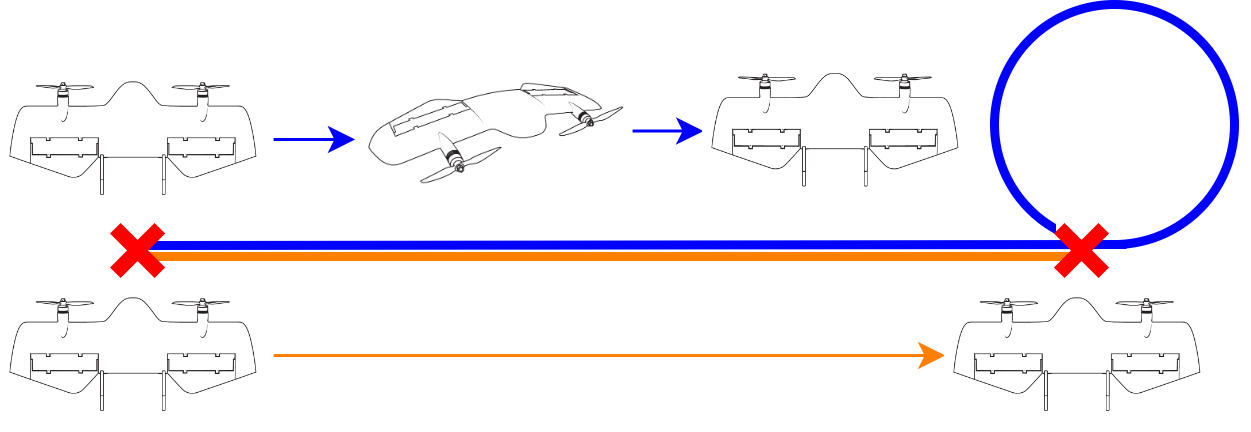
\includegraphics[trim=0cm 0cm 0cm 0cm,clip,width=0.8\columnwidth]{figures/DroneConvertibleGuidage.png}}
    \caption{Schéma de déplacement d'un drone convertible.}
    \label{fig:pbhybride}
\end{figure}





%%%%%%%% 6. APPENDIX %%%%%%%%
\appendix

% LTeX: enabled=true
\chapter*{Annexe technique sur les drones}
\addstarredchapter{Annexe technique sur les drones} 

\markboth{Annexe technique sur les drones}{Annexe technique sur les drones}

\renewcommand{\thefigure}{A.\arabic{figure}}
\setcounter{figure}{0} % Réinitialiser le compteur à 0

\renewcommand{\thetable}{A.\arabic{table}}
\setcounter{table}{0} % Réinitialiser le compteur à 0

\section*{Système de drone : Paparazzi}

Un drone est composé de plusieurs pièces assemblées entre elles pour former la structure sur laquelle sont fixés des actionneurs, un autopilote et une charge utile (colis, caméra, capteur, etc.). L'élément central est l'autopilote qui assure la communication entre tous les éléments. Nous pouvons décomposer l'autopilote en deux parties : la partie matérielle et la partie logicielle.
\nomenclature[]{\(PCB\)}{Circuit imprimé  \textit{Printed Circuit Board}}
La partie matérielle est constituée d'un circuit imprimé (PCB) sur lequel des composants sont installés pour assurer les tâches relatives au vol. La partie logicielle se décompose en deux éléments : le segment sol et le logiciel embarqué.

Nous pouvons détailler les capteurs embarqués et le microcontrôleur avec l'ensemble de ses ports de communication. 

 \subsection*{Les capteurs d'un autopilote}
 Un autopilote comporte généralement un accéléromètre, un gyroscope, un magnétomètre et un baromètre.
 
 \paragraph*{}
 \textbf{L'accéléromètre} à trois axes permet de mesurer l'ensemble des forces appliquées sur le véhicule, à l'exception du poids. Il est possible d'obtenir la position du drone par double intégration de la mesure de l'accéléromètre. Toutefois, il convient de souligner que la position dérive rapidement en raison des bruits de mesure.

 \paragraph*{}
 \textbf{Le gyroscope} à trois axes permet de mesurer les vitesses de rotation du véhicule. Il est possible d'obtenir l'orientation du drone par intégration de la mesure du gyroscope. Toutefois, comme précédemment, l'orientation dérive rapidement en raison des bruits de mesure.

 \paragraph*{}
 \textbf{Le magnétomètre} à trois axes indique la direction du nord magnétique. Il permet de se diriger par rapport à une référence connue. Le principal inconvénient de ce capteur est sa perturbation par les masses magnétiques environnantes, ainsi que par les champs magnétiques parasites induits par la proximité des moteurs électriques par exemple. Il est donc difficile de les utiliser à l'intérieur d'un bâtiment. L'influence magnétique de l'engin porteur et les perturbations dues à d'éventuels moteurs électriques peuvent être éliminées en qualifiant, de manière statique, les erreurs dues aux masses métalliques du véhicule et aux moteurs électriques (en fonction des tensions et courants d'alimentation).

 \paragraph*{}

 \textbf{Le baromètre} est un capteur d'altitude basé sur la mesure de la pression atmosphérique. Cette pression est mesurée par un système électronique basé sur la résonance naturelle d'une pièce en alliage de nickel ou sur la modification de l'équilibre d'un pont de Wheatstone associé à un cristal de quartz sur lequel, par l'intermédiaire d'une capsule souple, s'exerce la pression atmosphérique. On déduit de la variation de pression atmosphérique une variation d'altitude à l'aide du modèle d'atmosphère standard qui nous indique qu'au niveau de la mer, la pression diminue de \SI{1}{\hecto\pascal} tous les \SI{8.5}{\meter}
 

 \paragraph*{}
 \textbf{Le GPS} est monté en extérieur de l'autopilote. Ce système de géopositionnement par satellite (\textit{Global Positioning System}) permet d'obtenir un positionnement absolu du drone. 

 \nomenclature[]{\(GPS\)}{Géo-positionnement par satellite (\textit{Global Positioning System})}
 \paragraph*{}
 Il est courant de retrouver plusieurs capteurs dans un même boitier, que l'on nomme centrale inertielle (Inertial Measurement Units, IMU). Ces dernières sont composées au minimum d'un accéléromètre 3-axes et d'un gyroscope 3-axes, mais il est courant de les trouver avec un magnétomètre 3-axes. 

 \nomenclature[]{\(IMU\)}{Centrales inertielles (\textit{Inertial Measurement Units})}

 \subsection*{Le microcontrôleur d'un autopilote}
 Le microcontrôleur (Microcontroller Unit, MCU) est la pièce maitresse de l'autopilote en ce qu'il permet d'effectuer l'ensemble des traitements nécessaires à la conduite du vol.

 \nomenclature[]{\(MCU\)}{Microcontrôleurs (\textit{Microcontroller Unit})}

 De plus, il possède plusieurs ports de communication pour récupérer les données des capteurs ou envoyer des ordres aux actionneurs.

La liaison série permet de relier deux équipements numériques pour qu'ils puissent s'échanger des informations. C'est le moyen de communication le plus simple. Toutefois, il contient un moyen de détection des erreurs tel que le bit de parité.

 Le protocole \textit{CAN} provient de l'industrie automobile. Il permet de raccorder à un même câble un grand nombre de calculateurs qui communiqueront donc à tour de rôle. Cette technique élimine le besoin de câbler des lignes dédiées pour chaque information à faire transiter (connexion point-à-point).

 Nous pouvons citer le \textit{Dshot} qui est un protocole de communication défini entre l'autopilote et l'ESC pour envoyer les commandes des moteurs. Les avancées sur ce protocole ont notamment permis la communication bidirectionnelle, permettant d'obtenir la vitesse des moteurs, leur consommation et d'autres informations.

 Enfin, le protocole \textit{I2C} est un bus de communication série simplifiant l'interconnexion de circuit intégré sur une même carte. Ce bus ne nécessite que deux fils pour être mis en place. Il n'est conçu que pour faire communiquer des équipements relativement proches (quelques centimètres).

 \subsection*{Évolutions}
 Les nombreux progrès dans les systèmes d'estimation état permettent de connaître précisément l'orientation et la position des drones pour assurer la stabilisation, le guidage et la navigation. Les progrès sont liés à l'amélioration continue des capteurs, notamment des centrales inertielles constituées d'un accéléromètre, d'un gyroscope et d'un magnétomètre.

La Table \ref{tab:autopilote_ev} montre l'évolution des vitesses des microcontrôleurs (Microcontroller Unit, MCU) \nomenclature[]{\(MCU\)}{Microcontrôleurs (\textit{Microcontroller Unit})} embarqués sur les autopilotes et de la réduction du bruit des capteurs inertiels.
\begin{table}[ht]
    \centering
    \begin{tabular}{|c|c|c|c|c|c|}
        \hline
        Type & Date & MCU & Vitesse & Capteur  & Bruit RMS \\
        \hline \hline
        \href{https://wiki.paparazziuav.org/wiki/Apogee/v1.00}{Apogee}  & 2013 & STM32F4 & 168 MHz & MPU-9150 & \begin{tabular}{ccc} Gyro : 0.06 dps \\
        Accel: 4 mg  \end{tabular}  \\
        \hline
        \href{https://wiki.paparazziuav.org/wiki/Chimera/v1.00}{Chimera} & 2016 & STM32F7 & 216 MHz &  MPU-9250 & \begin{tabular}{ccc} Gyro : 0.1  dps \\
        Accel: 8 mg  \end{tabular}\\
        \hline
        \href{https://wiki.paparazziuav.org/wiki/Tawaki/v1.10}{Tawaki 1} &2019 &  STM32F7 & 216 MHz  & ICM-20600 & \begin{tabular}{ccc} Gyro : 0.04 dps \\
        Accel: 1 mg  \end{tabular}\\
        \hline
        \href{https://wiki.paparazziuav.org/wiki/Tawaki/v2.01}{Tawaki 2} &2023 &  STM32H7 & 480 MHz & ICM-42688-P & \begin{tabular}{ccc} Gyro : 0.028 dps \\
        Accel: 0.70 mg  \end{tabular} \\
        \hline
    \end{tabular}
    \caption{Évolution des autopilotes Paparazzi sur dix ans.}
    \label{tab:autopilote_ev}
\end{table}

Sur une période de dix ans, nous pouvons observer que les microcontrôleurs ont doublé leur vitesse d'exécution, que les fabricants ont divisé par deux le bruit moyen sur les gyroscopes et par quatre le bruit moyen des accéléromètres.
Ces évolutions continues permettent une amélioration de l'estimation du drone utilisée pour la stabilisation. Il en résulte une stabilité accrue et de nouvelles possibilités pour la commande des drones.

 \subsection*{Les logiciels d'un autopilote}
 Tout le fonctionnement d'un drone repose sur le logiciel qui permet de le faire voler. Il se décompose en deux catégories : la partie sol et la partie embarquée.

 \subsection*{Le segment sol}

Le segment sol est un ensemble de logiciels permettant de monitorer l'état du drone et de lui envoyer des ordres. Il repose sur les informations échangées avec le drone au travers de la télémétrie. L'interface principale est la GCS \textit{Ground Control Station} (voir Figure \ref{fig:GCS}), laquelle assure la visualisation du drone sur la carte, ainsi que toutes les commandes nécessaires au vol (modification de point de passage, atterrissage, etc.). Elle est écrite en C++.

\begin{figure}[ht!]
    \centerline{
    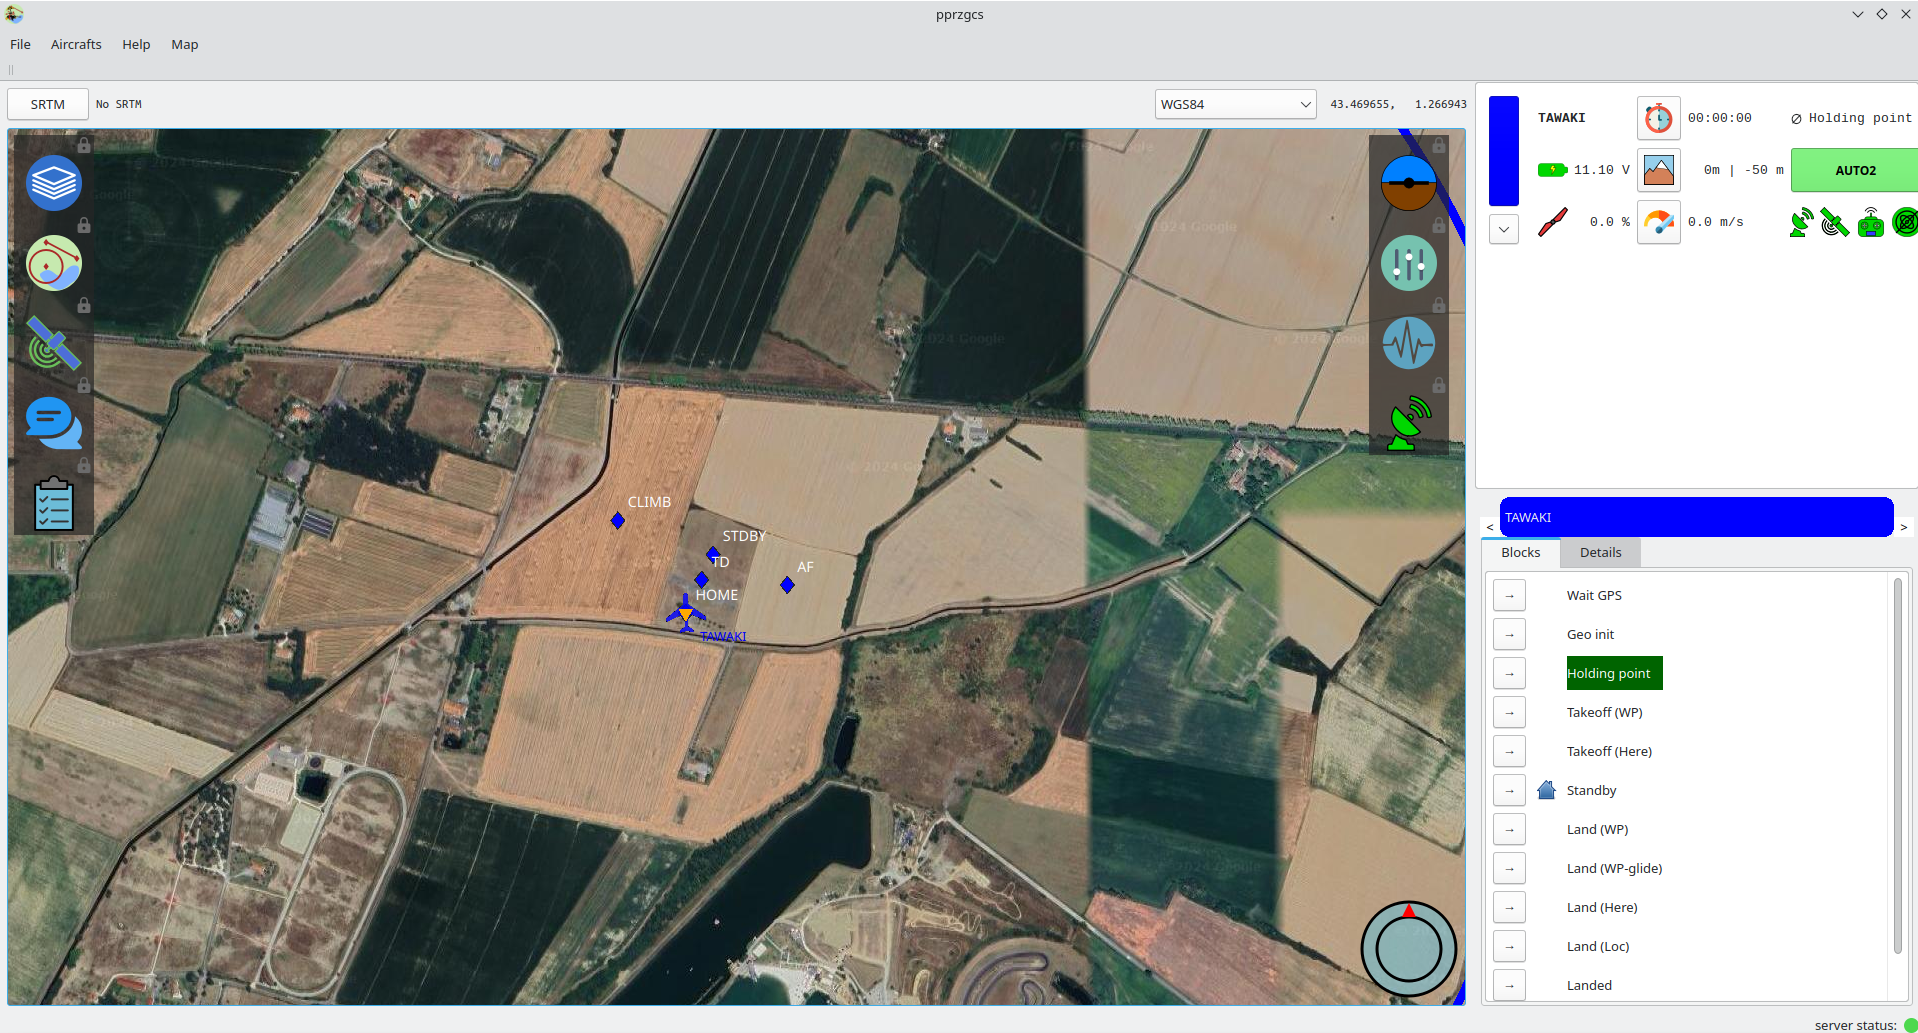
\includegraphics[trim=0cm 0cm 0cm 0cm,clip,width=0.8\columnwidth]{figures/GCS.png}}
    \caption{Interface graphique de la station de contrôle au sol.}
    \label{fig:GCS}
\end{figure}

\nomenclature[]{\(GCS\)}{Station de contrôle au sol \textit{Ground Control Station}}

Une autre partie du segment sol est le code serveur qui gère les messages échangés entre les différentes applications. Le code est en Ocaml.

Enfin, un code assure la compilation croisée du logiciel embarqué qui doit être téléversé sur le drone, basée sur des Makefile et du code Ocaml. Le logiciel embarqué est décrit par la suite.

 \subsection*{Le logiciel embarqué}
 Le logiciel embarqué est un code écrit en C, intégré dans un système d'exploitation temps réel "Chibios". Il est téléversé sur le microcontrôleur au travers d'une sonde de programmation ou de la prise USB présente sur l'autopilote.

 L'ensemble du code est organisé sous la forme de modules que l'on change au besoin. Chaque module assure des fonctionnalités telles que l'estimation d'état, la stabilisation, le guidage, la navigation ou encore la gestion de la charge utile (voir Figure \ref{fig:schedulingpaparazzi}). Grâce à un mécanisme de gestion de dépendance, les modules ont la possibilité de charger d'autres modules nécessaires à leur fonctionnement. L'ordre de compilation et d'édition des liens seront gérés par le logiciel de compilation.


 \begin{figure}[ht!]
    \centerline{
    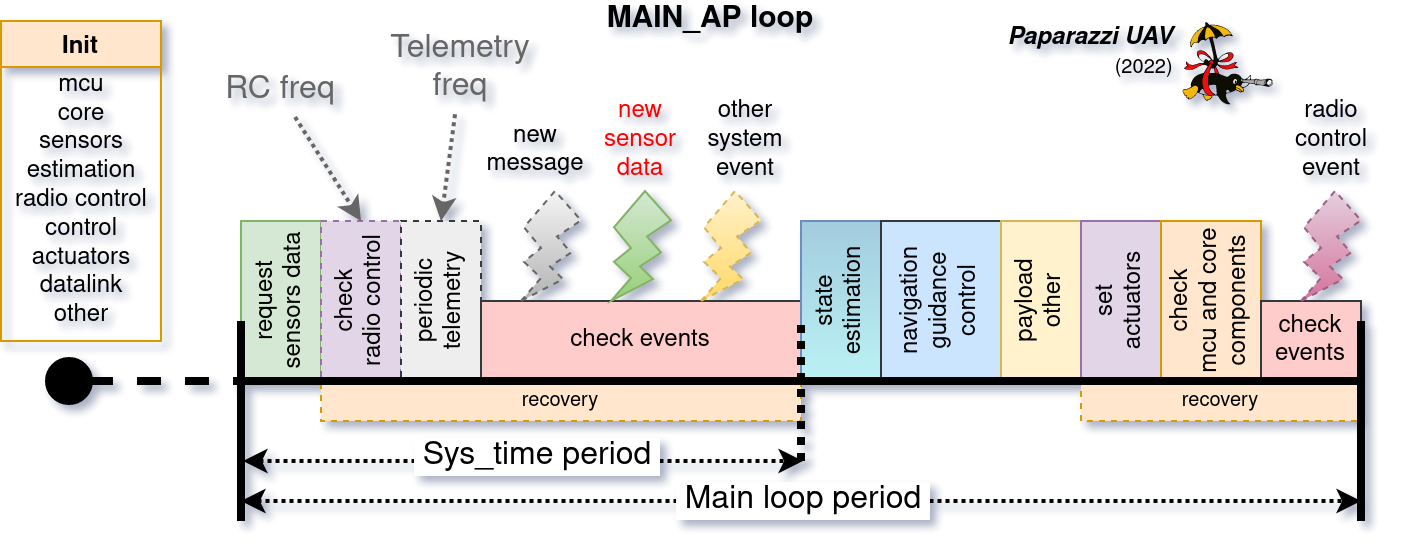
\includegraphics[trim=0cm 0cm 0cm 0cm,clip,width=0.7\columnwidth]{figures/PPRZ_Main_ap_loop.png}}
    \caption{Schéma de l'ordre d'exécution des codes embarqués \cite{RTDpaparazzi2022}.}
    \label{fig:schedulingpaparazzi}
\end{figure}

 
\section*{AM32}
Le logiciel AM32 est conçu pour les microprocesseurs ARM STM32 afin de contrôler un moteur \textit{brushless}, couramment utilisé pour les drones. Le logiciel est conçu pour être sûr et rapide, avec des démarrages rapides et sans à-coups et une accélération linéaire. Il est destiné à être utilisé avec plusieurs types de véhicules et de contrôleurs de vol. 

L'intérêt de ce logiciel est qu'il est ouvert, permettant de contribuer, en proposant des évolutions. Nous avons ainsi implémenté l'approche de \cite{franchi2017}, avec un algorithme de biais et de gain adaptatif (ABAG) (voir \ref{fig:ABAG_algo}).

\begin{figure}[ht!]
    \centerline{
    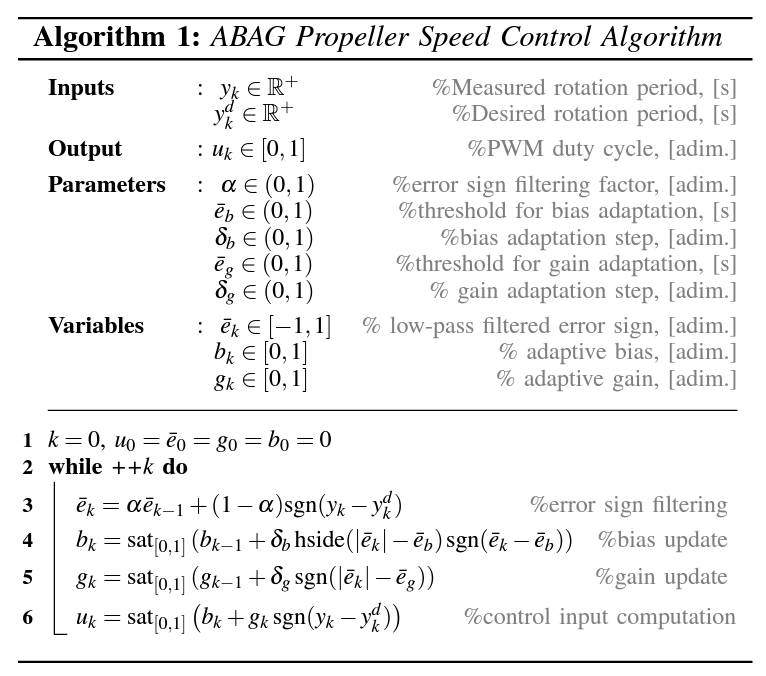
\includegraphics[trim=0cm 0cm 0cm 0cm,clip,width=0.6\columnwidth]{figures/ABAG_algo.png}}
    \caption{Algorithme de biais et de gain adaptatif (ABAG) \cite{franchi2017}.}
    \label{fig:ABAG_algo}
\end{figure}
L'algorithme ABAG est adaptatif et robuste en ce qu'il ne nécessite pas la connaissance des paramètres mécaniques ou électriques du groupe moteur et hélice et qu'il n'est pas nécessaire de procéder à une identification, ni de connaître l'entrée nominale. De plus, l'algorithme ABAG ne nécessite que très peu de ressources de calcul, ce qui en fait un atout important pour un système embarqué.

 % Revenir à la numérotation normale après la section si nécessaire
\renewcommand{\thefigure}{\thechapter.\arabic{figure}}
\renewcommand{\thetable}{\thechapter.\arabic{table}}

%%%%%%%% 7. BIBLIOGRAPHIE %%%%%%%%
\bibliographystyle{StyleThese}
%\bibliographystyle{plain}
\bibliography{biblio}


%%%%%%%% 8. LAST PAGE %%%%%%%%
\cleardoublepage
\pagestyle{empty} % remove headers on 2e page
\newgeometry{left=1.5in,right=1.3in,top=1.1in,bottom=1.1in} % remove header/footer space

% French
\begin{vcenterpage} % note: vcenterpage is not needed for long abstrat
\noindent\rule[2pt]{\textwidth}{0.5pt}

{\large\textbf{Résumé :}}
Les drones sont aujourd'hui devenus un outil dans de nombreux domaines tels que l'inspection, la surveillance ou la maintenance. Cependant, ils souffrent d'une autonomie limitée. Les \textit{tailsitters} apportent une solution grâce à leur grande enveloppe de vol et à leur efficacité énergétique. Toutefois, les \textit{tailsitters} sont grandement sujets aux perturbations aérologiques et notamment aux turbulences dans les phases stationnaires principalement. Cela est dû à la grande surface d'aile verticale, laquelle possède une grande prise au vent. De plus, leur corps tournant lors de la transition, il est donc compliqué de mesurer la vitesse de l'air.  Ainsi, en stationnaire ou à faible vitesse, le vent n'est pas connu. Ce type de drone est sous-actionné puisque l'on trouve deux moteurs sur l'aile et deux surfaces aérodynamiques sur le bord de fuite. Le flux d'air des hélices soufflant les élevons, nous avons un couplage entre les actionneurs.

Cette thèse cherche à étudier la commande de drones dans des environnements perturbés ou en présence de vent. Les premiers travaux se sont concentrés sur la dynamique sans vent pour appréhender une dynamique simplifiée. Nous avons pu proposer une modification non-linéaire du vecteur de commande pour rendre ce modèle linéaire en commande. De ce modèle, nous avons proposé une loi de commande locale-globale fondée sur une dynamique hybride à hystérésis. Elle permet d'étendre le domaine de stabilité de la loi de commande linéaire agressive à l'aide d'une loi non-linéaire avec une grande région d'attraction, mais moins agressive.

La suite des travaux s'est concentrée sur la stabilisation d'un \textit{tailsitters} soumis à des échelons de vent. Il en résulte une caractérisation des équilibres stationnaires pour un ensemble de conditions de vent et l'obtention de la représentation linéarisée de la dynamique du drone. À l'aide de ce modèle, il a été possible d'analyser les saturations des actionneurs et l'autorité disponible aux environs des points d'équilibre. Nous avons réalisé une stabilisation établie sur un retour de sortie, avec une action proportionnelle et intégrale. Cette commande n'utilise pas la mesure de l'angle de tangage du drone, car nous ne pouvons pas, a priori, connaître la valeur cible qui nécessiterait une estimation de la vitesse et de la direction du vent. L'optimisation de ce bouclage est effectuée à l'aide du logiciel "Systune" pour obtenir de bonnes propriétés de réjection de perturbation. Une approche incrémentale a été suivie, la loi de commande ayant été testée dans un premier temps sur une maquette à un degré de liberté face à une soufflerie ouverte. Une fois validée, la loi de commande a été implémentée dans le système de drone Paparazzi. Grâce à son architecture modulaire, il a été possible de nous interfacer avec les codes d'estimation et de commande des actionneurs. Ainsi, nous avons pu réaliser des vols sur le modèle complet à six degrés de liberté.

Enfin, nous avons proposé une architecture inspirée du \textit{tailsitter}, nommée \textit{freewing}. Nous avons développé un drone multicorps basé sur une aile en rotation libre sur son axe de tangage autour d'un fuselage. L'actionnement de l'aile est sensiblement le même que pour le \textit{tailsitters} et le fuselage possède deux actionneurs pour se maintenir horizontal. Nous recherchons, dans cette architecture, une passivité naturelle à la turbulence induite par le changement naturel de l'incidence de l'aile en fonction du vent incident. Il s'agit aussi d'installer une charge utile sur le fuselage horizontal sur le domaine de vol. De plus, nous avons réalisé un modèle de simulation où la dynamique est obtenue à l'aide des équations de Udwadia-Kalaba et de la phi-théorie. Enfin, nous nous sommes concentrés sur la stabilisation et le guidage du drone en utilisant une inversion incrémentale non-linéaire de la dynamique (INDI). Nous utilisons les actionneurs de l'aile et du fuselage pour obtenir une loi de stabilisation globale. Des vols ont validé l'intérêt de cette architecture.

{\large\textbf{Mots clés :}}
mots, clefs
\todo{Mots clés}

\noindent\rule[2pt]{\textwidth}{0.5pt}
\end{vcenterpage}

% English
\newpage
\begin{vcenterpage}
\noindent\rule[2pt]{\textwidth}{0.5pt}
% LTeX: language=en
{\large\textbf{Abstract:}}
Drones have become a prevalent tool in numerous fields, including inspection, surveillance, and maintenance. However, one area where they are currently lacking is autonomy. Tailsitter offer a viable solution, combining large flight envelopes with energy efficiency. Nonetheless, tailsitter unmanned aerial vehicles are particularly susceptible to disturbances, specifically turbulence during hover phases. This is because of the large vertical surface area of the wing, which offers a high degree of wind resistance. Furthermore, the drone's body rotates during transition, making it difficult to accurately measure airspeed. It is not possible to accurately measure wind speed, whether the drone is hovering or moving at a low speed. Additionally, this underactuated drone, has two motors on the wing and two aerodynamic surfaces on the trailing edge. The interaction of the airflow from the propellers with the elevons results in a coupling between the actuators.

The aim of this thesis is to examine the control of drone in challenging environments, with a particular emphasis on the impact of wind. However, initial research focused on windless dynamics in order to gain a better understanding of the simplified dynamics. We were able to propose a non-linear modification of the control vector to transform this nonlinear model into an input-affine model. Based on this model, we proposed a local-global control law based on hybrid dynamics with hysteresis, which allowed us to extend the stability domain of an aggressive linear control law by means of a non-linear law with a large region of attraction, but which was less aggressive. 

Further work was conducted on the stabilization of a tailsitter drone under wind steps. This resulted in a characterization of stationary equilibria for a range of wind conditions and a linearized representation of the drone's dynamics. Using this model, we were able to analyze the saturation levels of actuators and the authority available close to the equilibrium points. We have implemented a stabilization system based on output feedback with proportional and integral action, derived from the model. This control does not utilize the drones pitch angle measurement, since the target value is not known a priori. It would require an estimation of wind speed and direction, which is not feasible. The loop is optimized using "Systune" software in order to achieve effective disturbance rejection properties. We adopted an incremental approach by initially evaluating the control law on a one-degree-of-freedom model against an open wind tunnel. Upon validation, we proceeded to implement the control law within the Paparazzi UAV system. Due to its modular design, we were able to establish a connection with the state estimation and actuators, enabling us to execute flights on the entire model with six degrees of freedom. 

We then proposed an architecture inspired by the tailsitter, called freewing. We have developed a multi-body drone that is based on a wing that can freely rotate on its pitch axis around a fuselage. The wing is driven the same way as the tailsitter, and the fuselage has a motor and an aerodynamic surface to keep it horizontal. With this architecture, we aim to achieve a natural passivity to turbulence induced by the natural change in wing incidence as a function of the incident wind. However, there is also the possibility of installing a payload on the horizontal fuselage. To obtain a simulation model, we have modeled the drone's dynamics using the Udwadia-Kalaba equations and the phi-theory. We focused on stabilization and guidance of the UAV through the use of incremental nonlinear dynamic inversion (INDI). The wing and fuselage actuators are used to achieve a global stabilization law. In order to evaluate the benefits of this architecture, we conducted flight tests.

{\large\textbf{Keywords:}}
key, words
\todo{Keywords}

\noindent\rule[2pt]{\textwidth}{0.5pt}
\end{vcenterpage}


\end{document}
